% Options for packages loaded elsewhere
\PassOptionsToPackage{unicode}{hyperref}
\PassOptionsToPackage{hyphens}{url}
%
\documentclass[
]{book}
\usepackage{amsmath,amssymb}
\usepackage{lmodern}
\usepackage{ifxetex,ifluatex}
\ifnum 0\ifxetex 1\fi\ifluatex 1\fi=0 % if pdftex
  \usepackage[T1]{fontenc}
  \usepackage[utf8]{inputenc}
  \usepackage{textcomp} % provide euro and other symbols
\else % if luatex or xetex
  \usepackage{unicode-math}
  \defaultfontfeatures{Scale=MatchLowercase}
  \defaultfontfeatures[\rmfamily]{Ligatures=TeX,Scale=1}
\fi
% Use upquote if available, for straight quotes in verbatim environments
\IfFileExists{upquote.sty}{\usepackage{upquote}}{}
\IfFileExists{microtype.sty}{% use microtype if available
  \usepackage[]{microtype}
  \UseMicrotypeSet[protrusion]{basicmath} % disable protrusion for tt fonts
}{}
\makeatletter
\@ifundefined{KOMAClassName}{% if non-KOMA class
  \IfFileExists{parskip.sty}{%
    \usepackage{parskip}
  }{% else
    \setlength{\parindent}{0pt}
    \setlength{\parskip}{6pt plus 2pt minus 1pt}}
}{% if KOMA class
  \KOMAoptions{parskip=half}}
\makeatother
\usepackage{xcolor}
\IfFileExists{xurl.sty}{\usepackage{xurl}}{} % add URL line breaks if available
\IfFileExists{bookmark.sty}{\usepackage{bookmark}}{\usepackage{hyperref}}
\hypersetup{
  pdftitle={Modul Praktikum - Pelatihan Analisis Spasial},
  pdfauthor={Anik Djuraidah, Rahma Anisa, Gerry Alfa Dito},
  hidelinks,
  pdfcreator={LaTeX via pandoc}}
\urlstyle{same} % disable monospaced font for URLs
\usepackage{color}
\usepackage{fancyvrb}
\newcommand{\VerbBar}{|}
\newcommand{\VERB}{\Verb[commandchars=\\\{\}]}
\DefineVerbatimEnvironment{Highlighting}{Verbatim}{commandchars=\\\{\}}
% Add ',fontsize=\small' for more characters per line
\usepackage{framed}
\definecolor{shadecolor}{RGB}{248,248,248}
\newenvironment{Shaded}{\begin{snugshade}}{\end{snugshade}}
\newcommand{\AlertTok}[1]{\textcolor[rgb]{0.94,0.16,0.16}{#1}}
\newcommand{\AnnotationTok}[1]{\textcolor[rgb]{0.56,0.35,0.01}{\textbf{\textit{#1}}}}
\newcommand{\AttributeTok}[1]{\textcolor[rgb]{0.77,0.63,0.00}{#1}}
\newcommand{\BaseNTok}[1]{\textcolor[rgb]{0.00,0.00,0.81}{#1}}
\newcommand{\BuiltInTok}[1]{#1}
\newcommand{\CharTok}[1]{\textcolor[rgb]{0.31,0.60,0.02}{#1}}
\newcommand{\CommentTok}[1]{\textcolor[rgb]{0.56,0.35,0.01}{\textit{#1}}}
\newcommand{\CommentVarTok}[1]{\textcolor[rgb]{0.56,0.35,0.01}{\textbf{\textit{#1}}}}
\newcommand{\ConstantTok}[1]{\textcolor[rgb]{0.00,0.00,0.00}{#1}}
\newcommand{\ControlFlowTok}[1]{\textcolor[rgb]{0.13,0.29,0.53}{\textbf{#1}}}
\newcommand{\DataTypeTok}[1]{\textcolor[rgb]{0.13,0.29,0.53}{#1}}
\newcommand{\DecValTok}[1]{\textcolor[rgb]{0.00,0.00,0.81}{#1}}
\newcommand{\DocumentationTok}[1]{\textcolor[rgb]{0.56,0.35,0.01}{\textbf{\textit{#1}}}}
\newcommand{\ErrorTok}[1]{\textcolor[rgb]{0.64,0.00,0.00}{\textbf{#1}}}
\newcommand{\ExtensionTok}[1]{#1}
\newcommand{\FloatTok}[1]{\textcolor[rgb]{0.00,0.00,0.81}{#1}}
\newcommand{\FunctionTok}[1]{\textcolor[rgb]{0.00,0.00,0.00}{#1}}
\newcommand{\ImportTok}[1]{#1}
\newcommand{\InformationTok}[1]{\textcolor[rgb]{0.56,0.35,0.01}{\textbf{\textit{#1}}}}
\newcommand{\KeywordTok}[1]{\textcolor[rgb]{0.13,0.29,0.53}{\textbf{#1}}}
\newcommand{\NormalTok}[1]{#1}
\newcommand{\OperatorTok}[1]{\textcolor[rgb]{0.81,0.36,0.00}{\textbf{#1}}}
\newcommand{\OtherTok}[1]{\textcolor[rgb]{0.56,0.35,0.01}{#1}}
\newcommand{\PreprocessorTok}[1]{\textcolor[rgb]{0.56,0.35,0.01}{\textit{#1}}}
\newcommand{\RegionMarkerTok}[1]{#1}
\newcommand{\SpecialCharTok}[1]{\textcolor[rgb]{0.00,0.00,0.00}{#1}}
\newcommand{\SpecialStringTok}[1]{\textcolor[rgb]{0.31,0.60,0.02}{#1}}
\newcommand{\StringTok}[1]{\textcolor[rgb]{0.31,0.60,0.02}{#1}}
\newcommand{\VariableTok}[1]{\textcolor[rgb]{0.00,0.00,0.00}{#1}}
\newcommand{\VerbatimStringTok}[1]{\textcolor[rgb]{0.31,0.60,0.02}{#1}}
\newcommand{\WarningTok}[1]{\textcolor[rgb]{0.56,0.35,0.01}{\textbf{\textit{#1}}}}
\usepackage{longtable,booktabs,array}
\usepackage{calc} % for calculating minipage widths
% Correct order of tables after \paragraph or \subparagraph
\usepackage{etoolbox}
\makeatletter
\patchcmd\longtable{\par}{\if@noskipsec\mbox{}\fi\par}{}{}
\makeatother
% Allow footnotes in longtable head/foot
\IfFileExists{footnotehyper.sty}{\usepackage{footnotehyper}}{\usepackage{footnote}}
\makesavenoteenv{longtable}
\usepackage{graphicx}
\makeatletter
\def\maxwidth{\ifdim\Gin@nat@width>\linewidth\linewidth\else\Gin@nat@width\fi}
\def\maxheight{\ifdim\Gin@nat@height>\textheight\textheight\else\Gin@nat@height\fi}
\makeatother
% Scale images if necessary, so that they will not overflow the page
% margins by default, and it is still possible to overwrite the defaults
% using explicit options in \includegraphics[width, height, ...]{}
\setkeys{Gin}{width=\maxwidth,height=\maxheight,keepaspectratio}
% Set default figure placement to htbp
\makeatletter
\def\fps@figure{htbp}
\makeatother
\setlength{\emergencystretch}{3em} % prevent overfull lines
\providecommand{\tightlist}{%
  \setlength{\itemsep}{0pt}\setlength{\parskip}{0pt}}
\setcounter{secnumdepth}{5}
\usepackage{booktabs}
\usepackage{amsmath}
\usepackage{booktabs}
\usepackage{caption}
\usepackage{longtable}
\ifluatex
  \usepackage{selnolig}  % disable illegal ligatures
\fi
\usepackage[]{natbib}
\bibliographystyle{apalike}

\title{Modul Praktikum - Pelatihan Analisis Spasial}
\author{Anik Djuraidah, Rahma Anisa, Gerry Alfa Dito}
\date{17 dan 19 Maret 2021}

\begin{document}
\maketitle

{
\setcounter{tocdepth}{1}
\tableofcontents
}
\hypertarget{pengantar-analisis-spasial-dengan-r-software}{%
\chapter{Pengantar Analisis Spasial dengan R Software}\label{pengantar-analisis-spasial-dengan-r-software}}

\hypertarget{pengenalan-r-software}{%
\section{Pengenalan R Software}\label{pengenalan-r-software}}

Apabila Anda belum memiliki R dan RStudio pada perangkat PC atau laptop Anda, silahkan ikut langkah berikut:

\begin{enumerate}
\def\labelenumi{\arabic{enumi}.}
\item
  Download base R sesuai dengan \emph{operating system} Anda pada laman \url{https://cran.r-project.org}.
\item
  Install software tersebut pada system Anda.
\item
  Silahkan download versi desktop untuk RStudio pada system Anda pada laman berikut: \url{https://www.rstudio.com/products/RStudio/}.
\item
  Install RStudio pada system Anda.
\end{enumerate}

Setelah menginstall R dan Rstudio, selanjutnya anda akan menginstall package di R yang akan dibutuhkan dalam pelatihan ini. Langkah-langkah menginstallnya dapat dilihat pada video berikut

Daftar Package yang dibutuhkan dalam pelatihan ini adalah sebagai berikut

\begin{Shaded}
\begin{Highlighting}[]
\FunctionTok{install.packages}\NormalTok{(}\StringTok{"tidyverse"}\NormalTok{)}
\FunctionTok{install.packages}\NormalTok{(}\StringTok{"leafleat"}\NormalTok{)}
\FunctionTok{install.packages}\NormalTok{(}\StringTok{"sp"}\NormalTok{)}
\FunctionTok{install.packages}\NormalTok{(}\StringTok{"spData"}\NormalTok{)}
\FunctionTok{install.packages}\NormalTok{(}\StringTok{"spdep"}\NormalTok{)}
\FunctionTok{install.packages}\NormalTok{(}\StringTok{"rgdal"}\NormalTok{)}
\FunctionTok{install.packages}\NormalTok{(}\StringTok{"sf"}\NormalTok{)}
\FunctionTok{install.packages}\NormalTok{(}\StringTok{"GWmodel"}\NormalTok{)}
\FunctionTok{install.packages}\NormalTok{(}\StringTok{"spgwr"}\NormalTok{)}
\FunctionTok{install.packages}\NormalTok{(}\StringTok{"gwrr"}\NormalTok{)}
\FunctionTok{install.packages}\NormalTok{(}\StringTok{"plm"}\NormalTok{)}
\FunctionTok{install.packages}\NormalTok{(}\StringTok{"splm"}\NormalTok{)}
\end{Highlighting}
\end{Shaded}

Kemudian, berikut adalah daftar file yang harus didownload

\begin{enumerate}
\def\labelenumi{\arabic{enumi}.}
\tightlist
\item
  \href{https://github.com/raoy/Pelatihan-Spasial/raw/main/DATA\%20ATM\%20PONTIANAK.csv}{Data Atm Pontianak}
\item
  \href{https://github.com/raoy/Pelatihan-Spasial/raw/main/Data\%20SPBU\%20Pontianak.csv}{Data SPBU Pontianak}
\item
  \href{https://github.com/raoy/Pelatihan-Spasial/raw/main/Data\%20SPBU\%20Pontianak.xlsx}{Data SPBU Pontianak Excel}
\item
  \href{https://github.com/raoy/Pelatihan-Spasial/raw/main/P9\%20Dataset\%201.xlsx}{P9 Dataset 1}
\item
  \href{https://github.com/raoy/Pelatihan-Spasial/raw/main/Pulau\%20Jawa.csv}{Pulau Jawa}
\item
  \href{https://github.com/raoy/Pelatihan-Spasial/raw/main/metromanila.csv}{Metro Manila}
\item
  \href{https://github.com/raoy/Pelatihan-Spasial/raw/main/Jawamap.zip}{Peta Jawa}
\item
  \href{https://github.com/raoy/Pelatihan-Spasial/raw/main/Peta\%20Pontianak.zip}{Peta Pontianak}
\item
  \href{https://github.com/raoy/Pelatihan-Spasial/raw/main/SnowGIS_SHP.zip}{ShowGIS SHP}
\end{enumerate}

Setelah mendownload file-file diatas silahkan taruh file-file tersebut dalam satu folder dan file yang masih dalam bentuk \texttt{zip} silahkan extract terlebih dahulu. Kemudian silahkan jalankan sintaks dibawah ini

\begin{Shaded}
\begin{Highlighting}[]
\FunctionTok{setwd}\NormalTok{(}\StringTok{"D:/Research (eksternal dept)/pelatihan spasial (adj)/modul"}\NormalTok{)}
\end{Highlighting}
\end{Shaded}

\textbf{Tolong sesuaikan directori-nya dengan folder yang memuat file-file yang sudah didownload sebelumnya}

\hypertarget{cara-untuk-assignment-di-r}{%
\subsection{Cara untuk assignment di R}\label{cara-untuk-assignment-di-r}}

\begin{Shaded}
\begin{Highlighting}[]
\NormalTok{A }\OtherTok{\textless{}{-}} \DecValTok{5}
\NormalTok{A }\OtherTok{=} \DecValTok{5}
\DecValTok{5} \OtherTok{{-}\textgreater{}}\NormalTok{ A}
\FunctionTok{assign}\NormalTok{(}\StringTok{"A"}\NormalTok{,}\DecValTok{5}\NormalTok{)}
\NormalTok{A}
\end{Highlighting}
\end{Shaded}

\begin{verbatim}
## [1] 5
\end{verbatim}

Sintaks diatas berarti nilai 5 disimpan dalam Objek yang bernama A.

Beberapa aturan penamaan objek dalam R:

\begin{enumerate}
\def\labelenumi{\alph{enumi}.}
\tightlist
\item
  Case-Sensitive (Huruf A dengan a merupakan 2 objek berbeda).
\item
  Diawali huruf (A-Z atau a-z), misal A,dat1, a1.
\item
  Usahakan untuk tidak menggunakan nama fungsi yang sudah ada di R, seperti plot, lm, data,boxplot.
\end{enumerate}

\hypertarget{objek-data-standar-di-r}{%
\subsection{Objek Data Standar di R}\label{objek-data-standar-di-r}}

R memiliki 6 cara untuk menyimpan data dalam bentuk objek, yaitu \texttt{vector},\texttt{factor},\texttt{matrix}, \texttt{array}, \texttt{data.frame}, dan \texttt{list}.

\begin{enumerate}
\def\labelenumi{\arabic{enumi}.}
\tightlist
\item
  Vector
\end{enumerate}

Vector dalam R berisi elemen-element yang memiliki tipe data yang sama.

\begin{Shaded}
\begin{Highlighting}[]
\NormalTok{A }\OtherTok{\textless{}{-}} \FunctionTok{c}\NormalTok{(}\DecValTok{5}\NormalTok{, }\DecValTok{3}\NormalTok{, }\DecValTok{5}\NormalTok{, }\DecValTok{1}\NormalTok{)}
\NormalTok{x }\OtherTok{\textless{}{-}} \DecValTok{1}\SpecialCharTok{:}\DecValTok{10}
\NormalTok{n }\OtherTok{\textless{}{-}} \FunctionTok{c}\NormalTok{(}\StringTok{"a"}\NormalTok{, }\StringTok{\textquotesingle{}b\textquotesingle{}}\NormalTok{, }\StringTok{"c"}\NormalTok{)}
\NormalTok{y }\OtherTok{\textless{}{-}} \FunctionTok{seq}\NormalTok{(}\DecValTok{1}\NormalTok{, }\DecValTok{10}\NormalTok{, }\AttributeTok{by =} \DecValTok{2}\NormalTok{)}
\end{Highlighting}
\end{Shaded}

Kita bisa mengakses elemen-elemen vektor dengan cara berikut

\begin{Shaded}
\begin{Highlighting}[]
\NormalTok{A[}\DecValTok{3}\NormalTok{]}
\end{Highlighting}
\end{Shaded}

\begin{verbatim}
## [1] 5
\end{verbatim}

\begin{Shaded}
\begin{Highlighting}[]
\NormalTok{x[}\DecValTok{1}\SpecialCharTok{:}\DecValTok{4}\NormalTok{]}
\end{Highlighting}
\end{Shaded}

\begin{verbatim}
## [1] 1 2 3 4
\end{verbatim}

\begin{Shaded}
\begin{Highlighting}[]
\NormalTok{n[}\FunctionTok{c}\NormalTok{(}\DecValTok{1}\NormalTok{,}\DecValTok{3}\NormalTok{)]}
\end{Highlighting}
\end{Shaded}

\begin{verbatim}
## [1] "a" "c"
\end{verbatim}

\begin{Shaded}
\begin{Highlighting}[]
\NormalTok{y[}\SpecialCharTok{{-}}\NormalTok{(}\DecValTok{1}\SpecialCharTok{:}\DecValTok{2}\NormalTok{)]}
\end{Highlighting}
\end{Shaded}

\begin{verbatim}
## [1] 5 7 9
\end{verbatim}

\begin{enumerate}
\def\labelenumi{\arabic{enumi}.}
\setcounter{enumi}{1}
\tightlist
\item
  Factor
\end{enumerate}

Mirip dengan vector tapi mempunyai urutan (ordinal)

\begin{Shaded}
\begin{Highlighting}[]
\NormalTok{x }\OtherTok{\textless{}{-}} \FunctionTok{c}\NormalTok{(}\StringTok{"SD"}\NormalTok{, }\StringTok{"SMP"}\NormalTok{, }\StringTok{"SMA"}\NormalTok{, }\StringTok{"S1"}\NormalTok{)}
\NormalTok{sekolah }\OtherTok{\textless{}{-}} \FunctionTok{factor}\NormalTok{(x)}
\NormalTok{sekolah}
\end{Highlighting}
\end{Shaded}

\begin{verbatim}
## [1] SD  SMP SMA S1 
## Levels: S1 SD SMA SMP
\end{verbatim}

\begin{Shaded}
\begin{Highlighting}[]
\NormalTok{sekolah }\OtherTok{\textless{}{-}} \FunctionTok{factor}\NormalTok{(x, }\AttributeTok{levels =}\NormalTok{ x)}
\NormalTok{sekolah}
\end{Highlighting}
\end{Shaded}

\begin{verbatim}
## [1] SD  SMP SMA S1 
## Levels: SD SMP SMA S1
\end{verbatim}

Kita bisa mengakses elemen-elemen \texttt{factor} dengan cara berikut

\begin{Shaded}
\begin{Highlighting}[]
\NormalTok{sekolah[}\DecValTok{1}\NormalTok{] }
\end{Highlighting}
\end{Shaded}

\begin{verbatim}
## [1] SD
## Levels: SD SMP SMA S1
\end{verbatim}

\begin{Shaded}
\begin{Highlighting}[]
\NormalTok{sekolah[}\DecValTok{1}\SpecialCharTok{:}\DecValTok{2}\NormalTok{]}
\end{Highlighting}
\end{Shaded}

\begin{verbatim}
## [1] SD  SMP
## Levels: SD SMP SMA S1
\end{verbatim}

\begin{Shaded}
\begin{Highlighting}[]
\NormalTok{sekolah[}\FunctionTok{c}\NormalTok{(}\DecValTok{1}\NormalTok{,}\DecValTok{4}\NormalTok{)]}
\end{Highlighting}
\end{Shaded}

\begin{verbatim}
## [1] SD S1
## Levels: SD SMP SMA S1
\end{verbatim}

\begin{enumerate}
\def\labelenumi{\arabic{enumi}.}
\setcounter{enumi}{2}
\tightlist
\item
  Matriks
\end{enumerate}

Matrix dalam R memiliki dua dimensi yaitu baris dan kolom. Matrix hanya bisa digunakan untuk menyimpan 1 jenis tipe data saja, misalnya \texttt{numeric}.

\begin{Shaded}
\begin{Highlighting}[]
\NormalTok{M }\OtherTok{\textless{}{-}} \FunctionTok{matrix}\NormalTok{(}\FunctionTok{c}\NormalTok{(}\DecValTok{1}\NormalTok{, }\DecValTok{0}\NormalTok{, }\DecValTok{0}\NormalTok{, }\DecValTok{0}\NormalTok{, }\DecValTok{1}\NormalTok{, }\DecValTok{0}\NormalTok{, }\DecValTok{0}\NormalTok{, }\DecValTok{0}\NormalTok{, }\DecValTok{1}\NormalTok{), }
        \AttributeTok{nrow =} \DecValTok{3}\NormalTok{, }\AttributeTok{ncol =} \DecValTok{3}\NormalTok{, }\AttributeTok{byrow =} \ConstantTok{TRUE}\NormalTok{)}
\NormalTok{M}
\end{Highlighting}
\end{Shaded}

\begin{verbatim}
##      [,1] [,2] [,3]
## [1,]    1    0    0
## [2,]    0    1    0
## [3,]    0    0    1
\end{verbatim}

Kita bisa mengakses elemen-elemen `matriks dengan cara berikut

\begin{Shaded}
\begin{Highlighting}[]
\NormalTok{M[}\DecValTok{3}\NormalTok{]}
\end{Highlighting}
\end{Shaded}

\begin{verbatim}
## [1] 0
\end{verbatim}

\begin{Shaded}
\begin{Highlighting}[]
\NormalTok{M[}\DecValTok{1}\NormalTok{, }\DecValTok{1}\NormalTok{]}
\end{Highlighting}
\end{Shaded}

\begin{verbatim}
## [1] 1
\end{verbatim}

\begin{Shaded}
\begin{Highlighting}[]
\NormalTok{M[}\DecValTok{1}\NormalTok{, ]}
\end{Highlighting}
\end{Shaded}

\begin{verbatim}
## [1] 1 0 0
\end{verbatim}

\begin{Shaded}
\begin{Highlighting}[]
\NormalTok{M[}\DecValTok{1}\NormalTok{, }\FunctionTok{c}\NormalTok{(}\DecValTok{1}\NormalTok{,}\DecValTok{3}\NormalTok{)]}
\end{Highlighting}
\end{Shaded}

\begin{verbatim}
## [1] 1 0
\end{verbatim}

\begin{Shaded}
\begin{Highlighting}[]
\NormalTok{M[, }\FunctionTok{c}\NormalTok{(}\DecValTok{1}\NormalTok{,}\DecValTok{3}\NormalTok{)]}
\end{Highlighting}
\end{Shaded}

\begin{verbatim}
##      [,1] [,2]
## [1,]    1    0
## [2,]    0    0
## [3,]    0    1
\end{verbatim}

\begin{enumerate}
\def\labelenumi{\arabic{enumi}.}
\setcounter{enumi}{3}
\tightlist
\item
  Array
\end{enumerate}

Array merupakan perluasan dari matrix dalam hal dimensi. Jika matrix hanya memiliki dua dimensi, array bisa terdiri dari banyak dimensi. Fungsi yang digunakan untuk mendefinisikan array di R adalah fungsi \texttt{array}.

\begin{Shaded}
\begin{Highlighting}[]
\NormalTok{BB }\OtherTok{\textless{}{-}} \FunctionTok{array}\NormalTok{(}\DecValTok{1}\SpecialCharTok{:}\DecValTok{12}\NormalTok{,}\AttributeTok{dim =} \FunctionTok{c}\NormalTok{(}\DecValTok{3}\NormalTok{,}\DecValTok{2}\NormalTok{,}\DecValTok{2}\NormalTok{)) }\CommentTok{\#array berdimensi 3}
\NormalTok{BB}
\end{Highlighting}
\end{Shaded}

\begin{verbatim}
## , , 1
## 
##      [,1] [,2]
## [1,]    1    4
## [2,]    2    5
## [3,]    3    6
## 
## , , 2
## 
##      [,1] [,2]
## [1,]    7   10
## [2,]    8   11
## [3,]    9   12
\end{verbatim}

\begin{Shaded}
\begin{Highlighting}[]
\NormalTok{CC }\OtherTok{\textless{}{-}} \FunctionTok{array}\NormalTok{(}\DecValTok{1}\SpecialCharTok{:}\DecValTok{24}\NormalTok{,}\FunctionTok{c}\NormalTok{(}\DecValTok{4}\NormalTok{,}\DecValTok{2}\NormalTok{,}\DecValTok{2}\NormalTok{,}\DecValTok{2}\NormalTok{)) }\CommentTok{\# array berdimensi 4}
\NormalTok{CC}
\end{Highlighting}
\end{Shaded}

\begin{verbatim}
## , , 1, 1
## 
##      [,1] [,2]
## [1,]    1    5
## [2,]    2    6
## [3,]    3    7
## [4,]    4    8
## 
## , , 2, 1
## 
##      [,1] [,2]
## [1,]    9   13
## [2,]   10   14
## [3,]   11   15
## [4,]   12   16
## 
## , , 1, 2
## 
##      [,1] [,2]
## [1,]   17   21
## [2,]   18   22
## [3,]   19   23
## [4,]   20   24
## 
## , , 2, 2
## 
##      [,1] [,2]
## [1,]    1    5
## [2,]    2    6
## [3,]    3    7
## [4,]    4    8
\end{verbatim}

Kita bisa mengakses elemen-elemen `matriks dengan cara berikut

\begin{Shaded}
\begin{Highlighting}[]
\NormalTok{BB[}\DecValTok{3}\NormalTok{]}
\end{Highlighting}
\end{Shaded}

\begin{verbatim}
## [1] 3
\end{verbatim}

\begin{Shaded}
\begin{Highlighting}[]
\NormalTok{BB[}\DecValTok{1}\NormalTok{, }\DecValTok{1}\NormalTok{,}\DecValTok{2}\NormalTok{]}
\end{Highlighting}
\end{Shaded}

\begin{verbatim}
## [1] 7
\end{verbatim}

\begin{Shaded}
\begin{Highlighting}[]
\NormalTok{CC[}\DecValTok{1}\NormalTok{,}\DecValTok{1}\NormalTok{,}\DecValTok{2}\NormalTok{,}\DecValTok{2}\NormalTok{]}
\end{Highlighting}
\end{Shaded}

\begin{verbatim}
## [1] 1
\end{verbatim}

\begin{enumerate}
\def\labelenumi{\arabic{enumi}.}
\setcounter{enumi}{4}
\tightlist
\item
  Data Frame
\end{enumerate}

Objek seperti tabel di Excel atau database SQL yang terdiri dari baris dan kolom. Tipe data kolom dapat berbeda-beda antar kolom.

\begin{Shaded}
\begin{Highlighting}[]
\NormalTok{x }\OtherTok{\textless{}{-}} \DecValTok{10}\SpecialCharTok{:}\DecValTok{1}
\NormalTok{y }\OtherTok{\textless{}{-}} \SpecialCharTok{{-}}\DecValTok{4}\SpecialCharTok{:}\DecValTok{5}
\NormalTok{q }\OtherTok{\textless{}{-}} \FunctionTok{c}\NormalTok{(}\StringTok{"Hockey"}\NormalTok{, }\StringTok{"Football"}\NormalTok{, }\StringTok{"Baseball"}\NormalTok{, }\StringTok{"Curling"}\NormalTok{, }\StringTok{"Rugby"}\NormalTok{,}\StringTok{"Lacrosse"}\NormalTok{, }\StringTok{"Basketball"}\NormalTok{, }\StringTok{"Tennis"}\NormalTok{, }\StringTok{"Cricket"}\NormalTok{, }\StringTok{"Soccer"}\NormalTok{)}
\NormalTok{theDF }\OtherTok{\textless{}{-}} \FunctionTok{data.frame}\NormalTok{(x, y, q)}
\NormalTok{theDF}
\end{Highlighting}
\end{Shaded}

\begin{verbatim}
##     x  y          q
## 1  10 -4     Hockey
## 2   9 -3   Football
## 3   8 -2   Baseball
## 4   7 -1    Curling
## 5   6  0      Rugby
## 6   5  1   Lacrosse
## 7   4  2 Basketball
## 8   3  3     Tennis
## 9   2  4    Cricket
## 10  1  5     Soccer
\end{verbatim}

\begin{Shaded}
\begin{Highlighting}[]
\NormalTok{theDF }\OtherTok{\textless{}{-}} \FunctionTok{data.frame}\NormalTok{(}\AttributeTok{first=}\NormalTok{x,}\AttributeTok{second=}\NormalTok{y,}\AttributeTok{sports=}\NormalTok{q)}
\NormalTok{theDF}
\end{Highlighting}
\end{Shaded}

\begin{verbatim}
##    first second     sports
## 1     10     -4     Hockey
## 2      9     -3   Football
## 3      8     -2   Baseball
## 4      7     -1    Curling
## 5      6      0      Rugby
## 6      5      1   Lacrosse
## 7      4      2 Basketball
## 8      3      3     Tennis
## 9      2      4    Cricket
## 10     1      5     Soccer
\end{verbatim}

Kita bisa mengakses elemen-elemen \texttt{data.frame} dengan cara berikut

\begin{Shaded}
\begin{Highlighting}[]
\NormalTok{theDF[}\DecValTok{1}\NormalTok{,}\DecValTok{3}\NormalTok{] }\CommentTok{\#baris 1 kolom 3}
\end{Highlighting}
\end{Shaded}

\begin{verbatim}
## [1] "Hockey"
\end{verbatim}

\begin{Shaded}
\begin{Highlighting}[]
\NormalTok{theDF[}\FunctionTok{c}\NormalTok{(}\FunctionTok{c}\NormalTok{(}\DecValTok{1}\NormalTok{,}\DecValTok{5}\NormalTok{),}\DecValTok{7}\SpecialCharTok{:}\DecValTok{10}\NormalTok{),] }\CommentTok{\#baris 1,5,7,8,9,10}
\end{Highlighting}
\end{Shaded}

\begin{verbatim}
##    first second     sports
## 1     10     -4     Hockey
## 5      6      0      Rugby
## 7      4      2 Basketball
## 8      3      3     Tennis
## 9      2      4    Cricket
## 10     1      5     Soccer
\end{verbatim}

\begin{Shaded}
\begin{Highlighting}[]
\NormalTok{theDF[,}\FunctionTok{c}\NormalTok{(}\DecValTok{1}\NormalTok{,}\DecValTok{3}\NormalTok{)] }\CommentTok{\#kolom 1 dan 3}
\end{Highlighting}
\end{Shaded}

\begin{verbatim}
##    first     sports
## 1     10     Hockey
## 2      9   Football
## 3      8   Baseball
## 4      7    Curling
## 5      6      Rugby
## 6      5   Lacrosse
## 7      4 Basketball
## 8      3     Tennis
## 9      2    Cricket
## 10     1     Soccer
\end{verbatim}

\begin{Shaded}
\begin{Highlighting}[]
\NormalTok{theDF}\SpecialCharTok{$}\NormalTok{sports }\CommentTok{\#mengakses kolom sports}
\end{Highlighting}
\end{Shaded}

\begin{verbatim}
##  [1] "Hockey"     "Football"   "Baseball"   "Curling"    "Rugby"     
##  [6] "Lacrosse"   "Basketball" "Tennis"     "Cricket"    "Soccer"
\end{verbatim}

\begin{Shaded}
\begin{Highlighting}[]
\NormalTok{theDF[,}\FunctionTok{c}\NormalTok{(}\StringTok{"first"}\NormalTok{,}\StringTok{"sports"}\NormalTok{)] }\CommentTok{\#mengakses kolom first dan sports}
\end{Highlighting}
\end{Shaded}

\begin{verbatim}
##    first     sports
## 1     10     Hockey
## 2      9   Football
## 3      8   Baseball
## 4      7    Curling
## 5      6      Rugby
## 6      5   Lacrosse
## 7      4 Basketball
## 8      3     Tennis
## 9      2    Cricket
## 10     1     Soccer
\end{verbatim}

\hypertarget{mengakses-bantuan-di-r}{%
\subsection{Mengakses bantuan di R}\label{mengakses-bantuan-di-r}}

Untuk mengakses bantuan (help) dari suatu fungsi di R bisa menggunakan fungsi \texttt{help} atau operator tanda tanya \texttt{?}

\begin{Shaded}
\begin{Highlighting}[]
\FunctionTok{help}\NormalTok{(lm)}
\NormalTok{?plot}
\end{Highlighting}
\end{Shaded}

\hypertarget{pengenalan-data-spasial}{%
\section{Pengenalan Data Spasial}\label{pengenalan-data-spasial}}

Data spasial tidak hanya berisi baris dan kolom, namun objek geometrik, seperti titik, garis, ataupun poligon. Beberapa jenis data spasial adalah data titik, data kontinu, dan data area yang akan dibawah berikut ini. Sebelum membahas jenis data tersebut satu per satu, terlebih dulu akan dibahas struktur data spasial serta cara mengimpor data spasial ke dalam R.

\hypertarget{struktur-data-spasial}{%
\subsection{Struktur Data Spasial}\label{struktur-data-spasial}}

Tipe data spasial yang paling umum digunakan adalah \emph{shapefile}, adapun tipe lain yang juga cukup populer adalah KML (\emph{Keyhole Markup Language}). Data \emph{shapefile} sebenarnya terdiri dari beberapa file dengan beberapa extension, di antaranya adalah \texttt{.shp}, \texttt{.shx}, dan \texttt{.dbf}. Beberapa package yang umum digunakan untuk bekerja dengan data spasial adalah \texttt{sp} dan \texttt{rgdal}.

\hypertarget{ilustrasi-data-cholera}{%
\subsection{Ilustrasi Data Cholera}\label{ilustrasi-data-cholera}}

Sebagai ilustrasi, akan digunakan data yang tersedia pada laman \url{http://rtwilson.com/downloads/SnowGIS_SHP.zip}. Pastikan Anda mengekstrak folder data tersebut pada direktori yang Anda inginkan. Selanjutnya, package \texttt{rgdal} akan digunakan untuk membaca data \texttt{SnowGIS} tersebut.

\begin{Shaded}
\begin{Highlighting}[]
\FunctionTok{library}\NormalTok{(rgdal)}
\end{Highlighting}
\end{Shaded}

Untuk melihat file apa saja yang ada di dalam folder shapefile tersebut, kita dapat menggunakan fungsi \texttt{list.files()} dan tuliskan direktori Anda masing-masing, ini dikenal sebagai \textbf{dsn}.

\begin{Shaded}
\begin{Highlighting}[]
\NormalTok{dsn}\OtherTok{\textless{}{-}}\FunctionTok{paste}\NormalTok{(}\StringTok{"SnowGIS\_SHP/SnowGIS\_SHP"}\NormalTok{)}
\FunctionTok{list.files}\NormalTok{(dsn)}
\end{Highlighting}
\end{Shaded}

\begin{verbatim}
##  [1] "Cholera_Deaths.dbf"          "Cholera_Deaths.prj"         
##  [3] "Cholera_Deaths.sbn"          "Cholera_Deaths.sbx"         
##  [5] "Cholera_Deaths.shp"          "Cholera_Deaths.shx"         
##  [7] "OSMap.tfw"                   "OSMap.tif"                  
##  [9] "OSMap_Grayscale.tfw"         "OSMap_Grayscale.tif"        
## [11] "OSMap_Grayscale.tif.aux.xml" "OSMap_Grayscale.tif.ovr"    
## [13] "Pumps.dbf"                   "Pumps.prj"                  
## [15] "Pumps.sbx"                   "Pumps.shp"                  
## [17] "Pumps.shx"                   "README.txt"                 
## [19] "SnowMap.tfw"                 "SnowMap.tif"                
## [21] "SnowMap.tif.aux.xml"         "SnowMap.tif.ovr"
\end{verbatim}

Terlihat pada output di atas bahwa folder tersebut memuat beberapa shapefile, di antaranya terdapat 6 file dengan nama \texttt{Cholera\_Deaths}dan 5 file bernama \texttt{Pumps}. Kedua set data tersebut dikenal sebagai \textbf{layer}.

\begin{Shaded}
\begin{Highlighting}[]
\FunctionTok{ogrListLayers}\NormalTok{(dsn)}
\end{Highlighting}
\end{Shaded}

\begin{verbatim}
## [1] "Cholera_Deaths" "Pumps"         
## attr(,"driver")
## [1] "ESRI Shapefile"
## attr(,"nlayers")
## [1] 2
\end{verbatim}

Kita dapat menggunakan fungsi \texttt{ogrInfo()} untuk mengetahui informasi mengenai layer tersebut.

\begin{Shaded}
\begin{Highlighting}[]
\FunctionTok{ogrInfo}\NormalTok{(dsn, }\AttributeTok{layer =} \StringTok{"Cholera\_Deaths"}\NormalTok{)}
\end{Highlighting}
\end{Shaded}

\begin{verbatim}
## Source: "D:\Jobs\Pelatihan Spasial STIS\New folder\Pelatihan-Spasial\SnowGIS_SHP\SnowGIS_SHP", layer: "Cholera_Deaths"
## Driver: ESRI Shapefile; number of rows: 250 
## Feature type: wkbPoint with 2 dimensions
## Extent: (529160.3 180857.9) - (529655.9 181306.2)
## CRS: +proj=tmerc +lat_0=49 +lon_0=-2 +k=0.9996012717 +x_0=400000 +y_0=-100000 +ellps=airy +units=m +no_defs 
## LDID: 87 
## Number of fields: 2 
##    name type length typeName
## 1    Id    0      6  Integer
## 2 Count    0      4  Integer
\end{verbatim}

Fungsi \texttt{readOGR()} dapat digunakan untuk membaca data shapefile.

\begin{Shaded}
\begin{Highlighting}[]
\NormalTok{CholeraDeaths }\OtherTok{\textless{}{-}} \FunctionTok{readOGR}\NormalTok{(dsn, }\AttributeTok{layer =} \StringTok{"Cholera\_Deaths"}\NormalTok{)}
\end{Highlighting}
\end{Shaded}

\begin{verbatim}
## OGR data source with driver: ESRI Shapefile 
## Source: "D:\Jobs\Pelatihan Spasial STIS\New folder\Pelatihan-Spasial\SnowGIS_SHP\SnowGIS_SHP", layer: "Cholera_Deaths"
## with 250 features
## It has 2 fields
\end{verbatim}

\begin{Shaded}
\begin{Highlighting}[]
\FunctionTok{summary}\NormalTok{(CholeraDeaths)}
\end{Highlighting}
\end{Shaded}

\begin{verbatim}
## Object of class SpatialPointsDataFrame
## Coordinates:
##                min      max
## coords.x1 529160.3 529655.9
## coords.x2 180857.9 181306.2
## Is projected: TRUE 
## proj4string :
## [+proj=tmerc +lat_0=49 +lon_0=-2 +k=0.9996012717 +x_0=400000
## +y_0=-100000 +ellps=airy +units=m +no_defs]
## Number of points: 250
## Data attributes:
##        Id        Count       
##  Min.   :0   Min.   : 1.000  
##  1st Qu.:0   1st Qu.: 1.000  
##  Median :0   Median : 1.000  
##  Mean   :0   Mean   : 1.956  
##  3rd Qu.:0   3rd Qu.: 2.000  
##  Max.   :0   Max.   :15.000
\end{verbatim}

Selanjutnya kita dapat memeriksa \texttt{class} dari data \texttt{CholeraDeaths} tersebut.

\begin{Shaded}
\begin{Highlighting}[]
\FunctionTok{class}\NormalTok{(CholeraDeaths)}
\end{Highlighting}
\end{Shaded}

\begin{verbatim}
## [1] "SpatialPointsDataFrame"
## attr(,"package")
## [1] "sp"
\end{verbatim}

Data tersebut merupakan \texttt{SpatialPointsDataFrame} yang termasuk \texttt{S4\ class}, maka untuk mengakses data slot perlu digunakan notasi \texttt{@}.

\begin{Shaded}
\begin{Highlighting}[]
\FunctionTok{str}\NormalTok{(CholeraDeaths}\SpecialCharTok{@}\NormalTok{data)}
\end{Highlighting}
\end{Shaded}

\begin{verbatim}
## 'data.frame':    250 obs. of  2 variables:
##  $ Id   : int  0 0 0 0 0 0 0 0 0 0 ...
##  $ Count: int  3 2 1 1 4 2 2 2 3 2 ...
\end{verbatim}

\hypertarget{visualisasi-data-cholera}{%
\subsection{Visualisasi Data Cholera}\label{visualisasi-data-cholera}}

Fungsi \texttt{plot()} dapat digunakan untuk membuat grafik paling sederhana dari data \texttt{CholeraDeaths}.

\begin{Shaded}
\begin{Highlighting}[]
\FunctionTok{par}\NormalTok{(}\AttributeTok{mfrow=}\FunctionTok{c}\NormalTok{(}\DecValTok{1}\NormalTok{,}\DecValTok{2}\NormalTok{))}
\FunctionTok{plot}\NormalTok{(CholeraDeaths)}
\FunctionTok{plot}\NormalTok{(CholeraDeaths, }\AttributeTok{pch=}\DecValTok{20}\NormalTok{, }\AttributeTok{col=}\StringTok{"steelblue"}\NormalTok{)}
\end{Highlighting}
\end{Shaded}

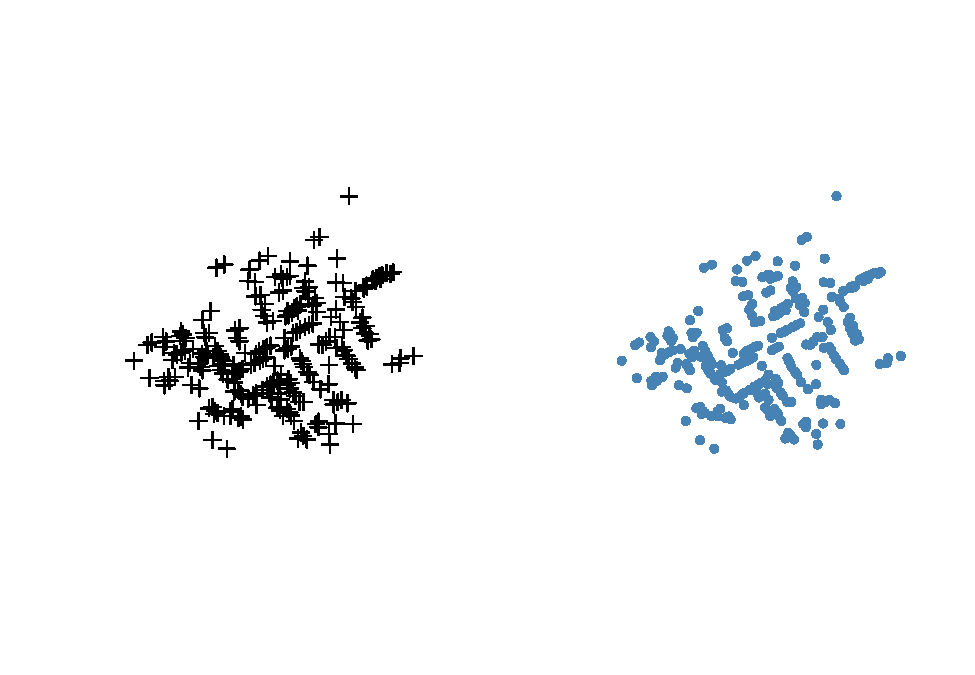
\includegraphics{modul_files/figure-latex/unnamed-chunk-22-1.pdf}

Perhatikan bahwa plot di atas hanya menunjukkan sebaran titik spasial, tanpa memberikan informasi yang jelas tentang lokasi data tersebut. Jika kita memiliki peta dalam bentuk data polygon, kita dapat mengimpor data tersebut dengan cara yang sama (seandainya datanya berupa shapefile), kemudian kita plot peta baru kemudian plot data titik seperti di atas.

Alternatif lainnya jika kita tidak ingin menggunakan peta polygon dari shapefile, kita dapat menggunakan beberapa package yang tersedia di R software, seperti \texttt{ggmap}, \texttt{OpenStreetMap}, \texttt{leaflet}, atau yang lain. Namun perhatikan bahwa untuk bisa menggunakan package \texttt{OpenStreetMap}, Anda harus memastikan bahwa jika Anda menggunakan \texttt{R} 64-bit maka \texttt{Java} yang terinstall di PC Anda juga harus sesuai, yaitu 64-bit.

Berikut ini akan ditunjukkan salah satu cara menampilkan peta dengan memanfaatkan package \texttt{leaflet}.

\begin{Shaded}
\begin{Highlighting}[]
\FunctionTok{library}\NormalTok{(leaflet)}
\NormalTok{map }\OtherTok{\textless{}{-}} \FunctionTok{leaflet}\NormalTok{() }\SpecialCharTok{\%\textgreater{}\%} \FunctionTok{setView}\NormalTok{(}\AttributeTok{lng =}  \SpecialCharTok{{-}}\FloatTok{0.13659}\NormalTok{, }\AttributeTok{lat =}\FloatTok{51.51328}\NormalTok{ , }\AttributeTok{zoom =} \DecValTok{12}\NormalTok{)}
\NormalTok{map }\SpecialCharTok{\%\textgreater{}\%} \FunctionTok{addTiles}\NormalTok{() }
\end{Highlighting}
\end{Shaded}

Sebelum kedua peta dan data titik digabungkan. Pastikan terlebih dahulu apakah koordinat yang digunakan menggunakan skala yang sama.

\begin{Shaded}
\begin{Highlighting}[]
\FunctionTok{head}\NormalTok{(}\FunctionTok{coordinates}\NormalTok{(CholeraDeaths))}
\end{Highlighting}
\end{Shaded}

\begin{verbatim}
##      coords.x1 coords.x2
## [1,]  529308.7  181031.4
## [2,]  529312.2  181025.2
## [3,]  529314.4  181020.3
## [4,]  529317.4  181014.3
## [5,]  529320.7  181007.9
## [6,]  529336.7  181006.0
\end{verbatim}

Seperti terlihat di atas, koordinat pada data \texttt{CholeraDeaths} diukur pada skala yang berbeda dengan peta yang diambil dari package \texttt{leaflet}. Terdapat beberapa macam \emph{coordinate reference system (CRS)}, beberapa di antaranya yang cukup populer adalah suatu set EPSG (\emph{European Petroleum Survey Group}) berikut:

\begin{itemize}
\item
  \textbf{EPSG:4326} juga dikenal sebagai WGS84, ukuran standard yang digunakan pada sistem GPS dan \emph{Google Earth}.
\item
  \textbf{EPSG:3857} digunakan pada Google Maps, Open Street Maps, dsb.
\item
  \textbf{EPSG:27700} juga dikenal sebagai OSGB 1936, atau \emph{British National Grid: United Kingdom Ordnance Survey}.
\end{itemize}

\begin{Shaded}
\begin{Highlighting}[]
\NormalTok{cholera\_latlong }\OtherTok{\textless{}{-}}\NormalTok{ CholeraDeaths }\SpecialCharTok{\%\textgreater{}\%} 
  \FunctionTok{spTransform}\NormalTok{(}\FunctionTok{CRS}\NormalTok{(}\StringTok{"+init=epsg:4326"}\NormalTok{))}
\FunctionTok{leaflet}\NormalTok{(}\AttributeTok{data =}\NormalTok{ CholeraDeaths) }\SpecialCharTok{\%\textgreater{}\%} 
  \FunctionTok{addTiles}\NormalTok{() }\SpecialCharTok{\%\textgreater{}\%}
  \FunctionTok{addMarkers}\NormalTok{(cholera\_latlong}\SpecialCharTok{@}\NormalTok{coords[,}\DecValTok{1}\NormalTok{], cholera\_latlong}\SpecialCharTok{@}\NormalTok{coords[,}\DecValTok{2}\NormalTok{])}
\end{Highlighting}
\end{Shaded}

Dapat dilihat di atas, bahwa setelah koordinatnya disamakan, kita dapat menampilkan data \texttt{CholeraDeaths} pada peta yang diperoleh dari \texttt{Open\ Street\ Map} melalui package \texttt{leaflet}.

\hypertarget{tipe-data-spasial}{%
\section{Tipe Data Spasial}\label{tipe-data-spasial}}

\hypertarget{tipe-data-titik}{%
\subsection{Tipe Data titik}\label{tipe-data-titik}}

Data spasial dapat berupa titik pengamatan pada lokasi tertentu, yang umumnya menyimpan koordinat lokasi \emph{longitude} dan \emph{latitude}. Data jenis ini hanya memiliki nilai pada titik tertentu saja, misalnya data kejadian kecelakaan, data rumah sakit, data kejadian kriminal, dan lain-lain. Sebagai ilustrasi, akan diperlihatkan data atm dan SPBU berikut ini.

\begin{Shaded}
\begin{Highlighting}[]
\FunctionTok{library}\NormalTok{(rgdal)}
\NormalTok{petapontianak}\OtherTok{=}\FunctionTok{readOGR}\NormalTok{(}\AttributeTok{dsn=}\StringTok{"Peta Pontianak"}\NormalTok{, }\AttributeTok{layer=}\StringTok{"Pontianak\_kec"}\NormalTok{)}
\end{Highlighting}
\end{Shaded}

\begin{verbatim}
## OGR data source with driver: ESRI Shapefile 
## Source: "D:\Jobs\Pelatihan Spasial STIS\New folder\Pelatihan-Spasial\Peta Pontianak", layer: "Pontianak_kec"
## with 6 features
## It has 1 fields
\end{verbatim}

\begin{Shaded}
\begin{Highlighting}[]
\NormalTok{dataATM}\OtherTok{=}\FunctionTok{read.csv}\NormalTok{(}\StringTok{"DATA ATM PONTIANAK.csv"}\NormalTok{ , }\AttributeTok{header=}\NormalTok{T)}
\NormalTok{dataSPBU}\OtherTok{=}\FunctionTok{read.csv}\NormalTok{(}\StringTok{"Data SPBU Pontianak.csv"}\NormalTok{, }\AttributeTok{sep=}\StringTok{";"}\NormalTok{,}\AttributeTok{header=}\NormalTok{T)}
\FunctionTok{plot}\NormalTok{(petapontianak)}
\FunctionTok{points}\NormalTok{(dataATM}\SpecialCharTok{$}\NormalTok{lon, dataATM}\SpecialCharTok{$}\NormalTok{lat, }\AttributeTok{col=}\StringTok{"blue"}\NormalTok{, }\AttributeTok{pch=}\DecValTok{3}\NormalTok{)}
\FunctionTok{points}\NormalTok{(dataSPBU}\SpecialCharTok{$}\NormalTok{lon, dataSPBU}\SpecialCharTok{$}\NormalTok{lat, }\AttributeTok{col=}\StringTok{"red"}\NormalTok{, }\AttributeTok{pch=}\DecValTok{3}\NormalTok{)}
\FunctionTok{title}\NormalTok{(}\StringTok{"Lokasi ATM dan SPBU di Pontianak"}\NormalTok{)}
\end{Highlighting}
\end{Shaded}

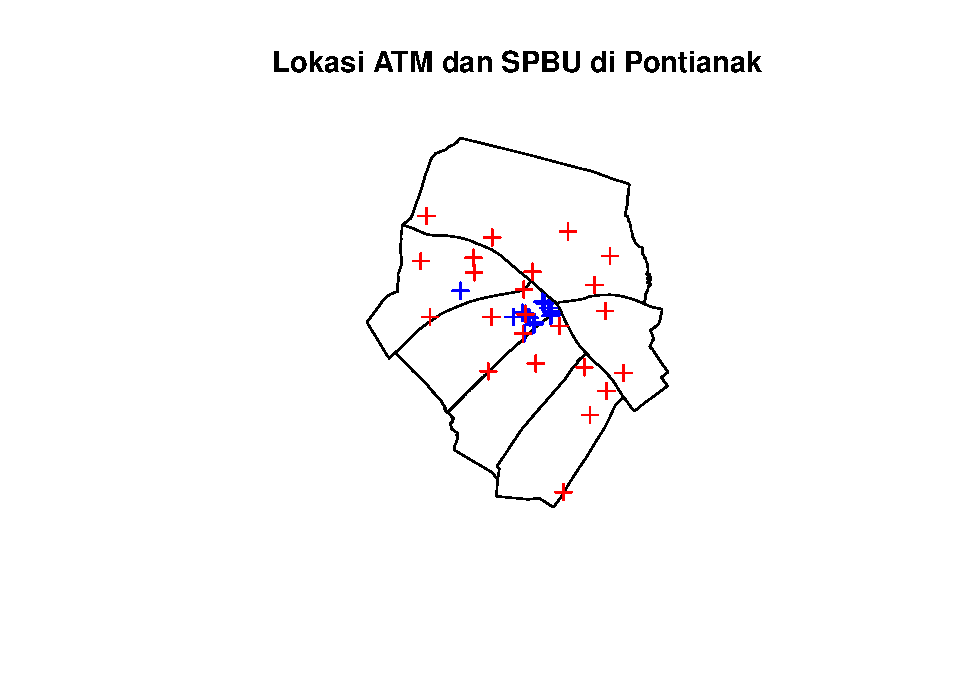
\includegraphics{modul_files/figure-latex/unnamed-chunk-26-1.pdf}

Data yang digunakan adalah berupa titik yang menunjukkan lokasi ATM dan SPBU. Lokasi ATM ditunjukkan dengan warna biru, sedangkan lokasi SPBU ditunjukkan dengan warna merah

\hypertarget{tipe-data-kontinu}{%
\subsection{Tipe Data Kontinu}\label{tipe-data-kontinu}}

Tipe data ini merupakan pengamatan yang memiliki nilai tidak hanya pada titik yang tersampel saja, namun nilai pengamatan sebenarnya kontinu untuk semua area. Artinya, di luar dari titik yang tersampel pun memiliki nilai untuk peubah yang diamati tersebut. Misalnya polusi udara, temperatur, kelembapan udara, presipitasi, dan sebagainya. Sebagai ilustrai, berikut ini adalah contoh data presipitasi di daerah Metro Manila.

\begin{Shaded}
\begin{Highlighting}[]
\FunctionTok{library}\NormalTok{(sp)}
\FunctionTok{library}\NormalTok{(gstat)}
\end{Highlighting}
\end{Shaded}

\begin{verbatim}
## Warning: package 'gstat' was built under R version 4.0.4
\end{verbatim}

\begin{Shaded}
\begin{Highlighting}[]
\NormalTok{metromanila}\OtherTok{=}\FunctionTok{read.csv}\NormalTok{(}\StringTok{"metromanila.csv"}\NormalTok{)}
\FunctionTok{coordinates}\NormalTok{(metromanila)}\OtherTok{\textless{}{-}}\FunctionTok{c}\NormalTok{(}\StringTok{"lon"}\NormalTok{,}\StringTok{"lat"}\NormalTok{)}
\FunctionTok{spplot}\NormalTok{(metromanila,}\StringTok{"precipitation"}\NormalTok{, }\AttributeTok{asp =} \DecValTok{1}\NormalTok{,}
       \AttributeTok{cex=}\FloatTok{0.5}\NormalTok{, }\AttributeTok{pch =} \DecValTok{19}\NormalTok{, }\AttributeTok{main=}\StringTok{"Angka Presipitasi di Metro Manila"}\NormalTok{)}
\end{Highlighting}
\end{Shaded}

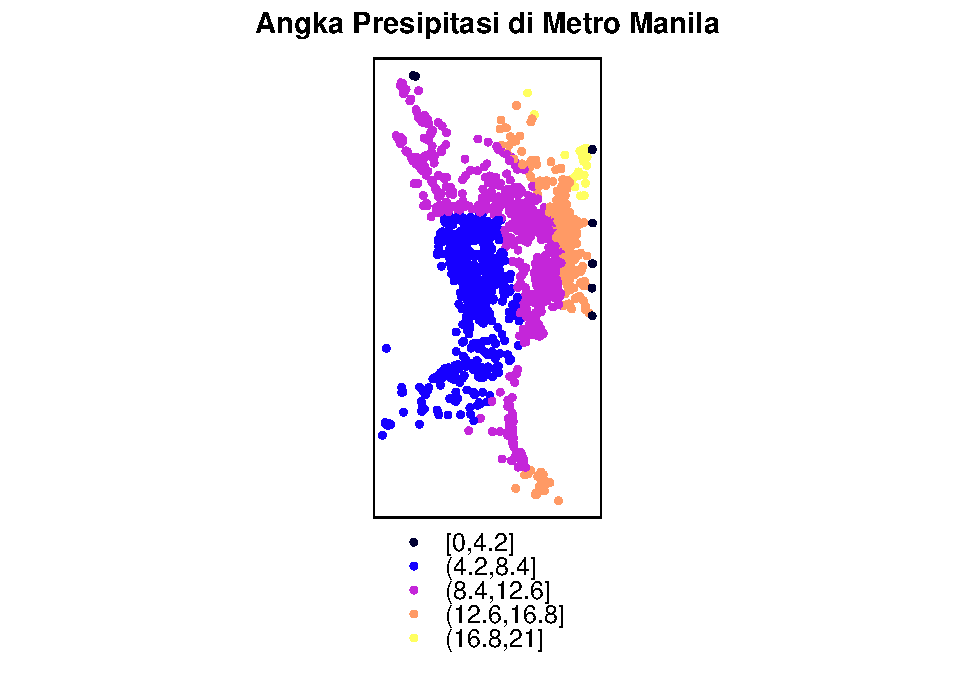
\includegraphics{modul_files/figure-latex/unnamed-chunk-27-1.pdf}

\hypertarget{tipe-data-area}{%
\subsection{Tipe Data Area}\label{tipe-data-area}}

Pada tipe data ini, pengamatan dilakukan pada level area. Area dapat mengacu pada sistem administrasi misalnya desa, kelurahan, kecamatan, kota, bahkan negara. Berikut ini adalah contoh data area yang diukur pada level kabupaten/kota. Untuk selanjutnya, pengamatan pada berbagai peubah dapat ditambahkan ke dalam data agar dapat diolah pada tahap analisis berikutnya.

\begin{Shaded}
\begin{Highlighting}[]
\FunctionTok{library}\NormalTok{(spdep)}
\FunctionTok{library}\NormalTok{(rgdal)}
\FunctionTok{library}\NormalTok{(raster)}
\NormalTok{petajawa}\OtherTok{\textless{}{-}} \FunctionTok{readOGR}\NormalTok{(}\AttributeTok{dsn =} \StringTok{"Jawamap"}\NormalTok{, }\AttributeTok{layer=}\StringTok{"jawa"}\NormalTok{)}
\end{Highlighting}
\end{Shaded}

\begin{verbatim}
## OGR data source with driver: ESRI Shapefile 
## Source: "D:\Jobs\Pelatihan Spasial STIS\New folder\Pelatihan-Spasial\Jawamap", layer: "jawa"
## with 119 features
## It has 5 fields
\end{verbatim}

\begin{Shaded}
\begin{Highlighting}[]
\FunctionTok{plot}\NormalTok{(petajawa)}
\end{Highlighting}
\end{Shaded}

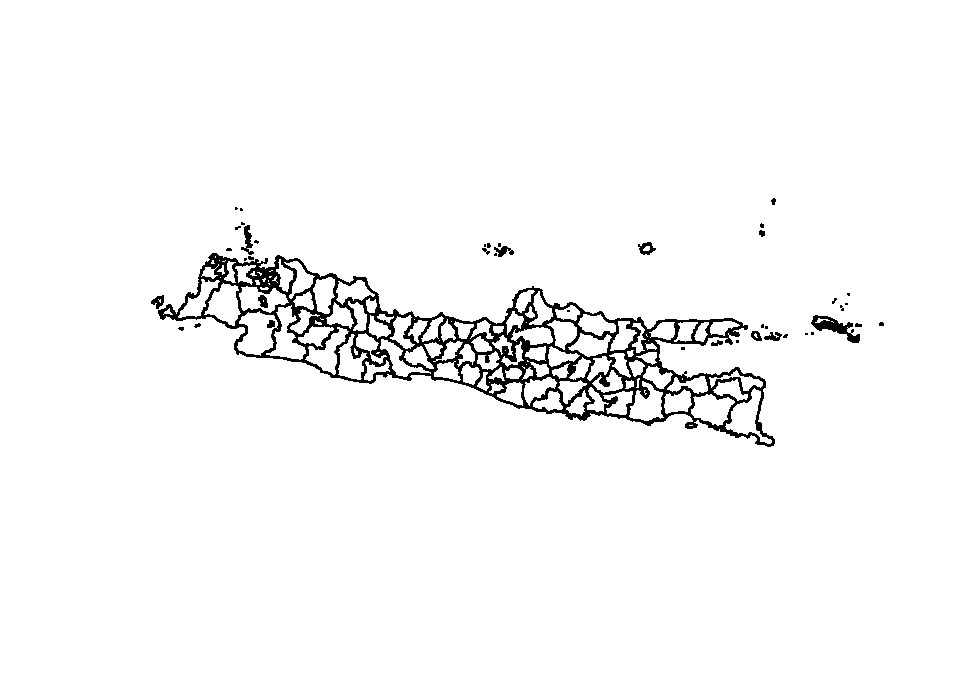
\includegraphics{modul_files/figure-latex/unnamed-chunk-28-1.pdf}

\hypertarget{matriks-bobot-dan-autokorelasi-spasial}{%
\section{Matriks Bobot dan Autokorelasi Spasial}\label{matriks-bobot-dan-autokorelasi-spasial}}

Pada analisis data spasial, informasi ketergantungan antar lokasi dapat diukur dengan autokorelasi spasial. Untuk dapat menghitung nilai autokorelasi tersebut, terdapat beberapa tahap yang perlu dilakukan, yaitu:

\begin{enumerate}
\def\labelenumi{(\arabic{enumi})}
\item
  menentukan kriteria kebertentanggaan antar lokasi pengamatan
\item
  menyusun matriks bobot spasial
\item
  matriks bobot spasial selanjutnya dapat dimanfaatkan baik untuk mengukur autokorelasi spasial maupun untuk menyusun pemodelan spasial.
\end{enumerate}

\hypertarget{kriteria-kebertetanggaan}{%
\subsection{Kriteria Kebertetanggaan}\label{kriteria-kebertetanggaan}}

Ilustrasi yang akan digunakan pada bagian ini adalah data yang tersedia di dalam R. Data tersebut dapat dipanggil dengan fungsi berikut.

\begin{Shaded}
\begin{Highlighting}[]
\FunctionTok{library}\NormalTok{(raster)}
\NormalTok{p }\OtherTok{\textless{}{-}} \FunctionTok{shapefile}\NormalTok{(}\FunctionTok{system.file}\NormalTok{(}\StringTok{"external/lux.shp"}\NormalTok{, }\AttributeTok{package=}\StringTok{"raster"}\NormalTok{))}
\NormalTok{p }\OtherTok{\textless{}{-}}\NormalTok{ p[p}\SpecialCharTok{$}\NormalTok{NAME\_1}\SpecialCharTok{==}\StringTok{"Diekirch"}\NormalTok{, ]}
\end{Highlighting}
\end{Shaded}

Selanjutnya kita akan tentukan sembarang nilai yang akan disimpan pada setiap lokasi untuk mengilustrasikan nilai peubah yang diamati.

\begin{Shaded}
\begin{Highlighting}[]
\NormalTok{p}\SpecialCharTok{$}\NormalTok{value }\OtherTok{\textless{}{-}} \FunctionTok{c}\NormalTok{(}\DecValTok{10}\NormalTok{, }\DecValTok{6}\NormalTok{, }\DecValTok{4}\NormalTok{, }\DecValTok{11}\NormalTok{, }\DecValTok{6}\NormalTok{)}
\FunctionTok{data.frame}\NormalTok{(p)}
\end{Highlighting}
\end{Shaded}

\begin{verbatim}
##   ID_1   NAME_1 ID_2   NAME_2 AREA value
## 0    1 Diekirch    1 Clervaux  312    10
## 1    1 Diekirch    2 Diekirch  218     6
## 2    1 Diekirch    3  Redange  259     4
## 3    1 Diekirch    4  Vianden   76    11
## 4    1 Diekirch    5    Wiltz  263     6
\end{verbatim}

Berikut adalah visualisasi dari data yang telah kita persiapkan.

\begin{Shaded}
\begin{Highlighting}[]
\FunctionTok{par}\NormalTok{(}\AttributeTok{mai=}\FunctionTok{c}\NormalTok{(}\DecValTok{0}\NormalTok{,}\DecValTok{0}\NormalTok{,}\DecValTok{0}\NormalTok{,}\DecValTok{0}\NormalTok{))}
\FunctionTok{plot}\NormalTok{(p, }\AttributeTok{col=}\DecValTok{2}\SpecialCharTok{:}\DecValTok{7}\NormalTok{)}
\NormalTok{coords }\OtherTok{\textless{}{-}} \FunctionTok{coordinates}\NormalTok{(p)}
\FunctionTok{points}\NormalTok{(coords, }\AttributeTok{cex=}\DecValTok{6}\NormalTok{, }\AttributeTok{pch=}\DecValTok{20}\NormalTok{, }\AttributeTok{col=}\StringTok{\textquotesingle{}white\textquotesingle{}}\NormalTok{)}
\FunctionTok{text}\NormalTok{(p, }\StringTok{\textquotesingle{}ID\_2\textquotesingle{}}\NormalTok{, }\AttributeTok{cex=}\FloatTok{1.5}\NormalTok{)}
\end{Highlighting}
\end{Shaded}

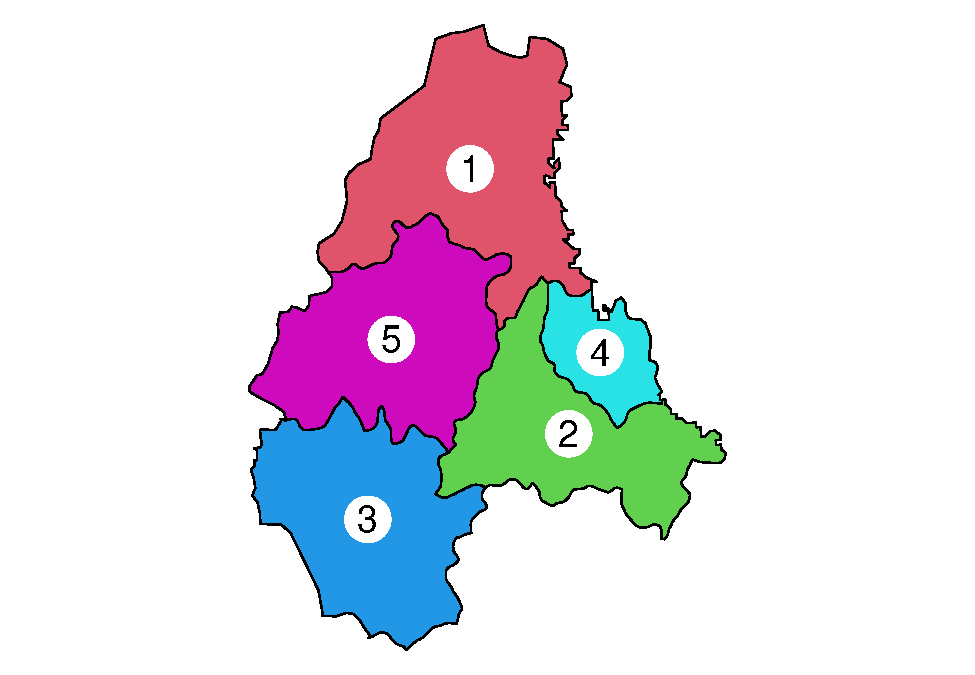
\includegraphics{modul_files/figure-latex/unnamed-chunk-31-1.pdf}

\hypertarget{contiguity-based}{%
\subsubsection{\texorpdfstring{\emph{Contiguity Based}}{Contiguity Based}}\label{contiguity-based}}

Kriteria yang umum digunakan pada ketetanggaan berbasis \emph{contiguity} adalah \emph{queen contiguity}, \emph{rook contiguity}, dan \emph{bishop contiguity}, seperti yang terlihat pada ilustrasi berikut ini.

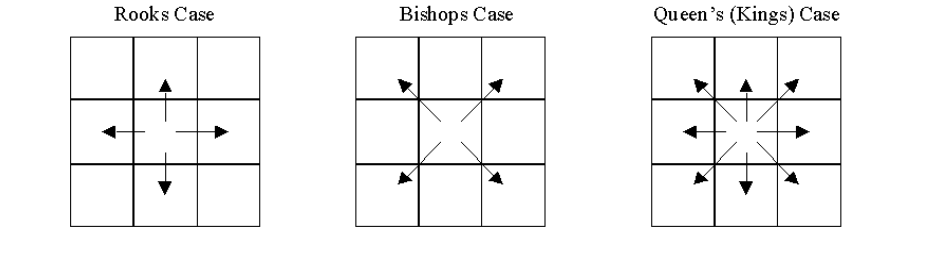
\includegraphics{D:/Research (eksternal dept)/pelatihan spasial (adj)/Modul Pelatihan Spasial/gambar 1.png}

Program berikut ini dapat diguakan untuk dapat memperoleh matriks bobot berdasarkan kriteria \emph{queen contiguity}.

\begin{Shaded}
\begin{Highlighting}[]
\FunctionTok{library}\NormalTok{(spdep)}
\NormalTok{w }\OtherTok{\textless{}{-}} \FunctionTok{poly2nb}\NormalTok{(p)}

\CommentTok{\#lebih lengkap dapat dituliskan seperti berikut ini:}
\NormalTok{w }\OtherTok{\textless{}{-}} \FunctionTok{poly2nb}\NormalTok{(p, }\AttributeTok{queen=}\ConstantTok{TRUE}\NormalTok{)}

\FunctionTok{plot}\NormalTok{(p)}
\FunctionTok{plot}\NormalTok{(w, coords, }\AttributeTok{add=}\NormalTok{T)}
\end{Highlighting}
\end{Shaded}

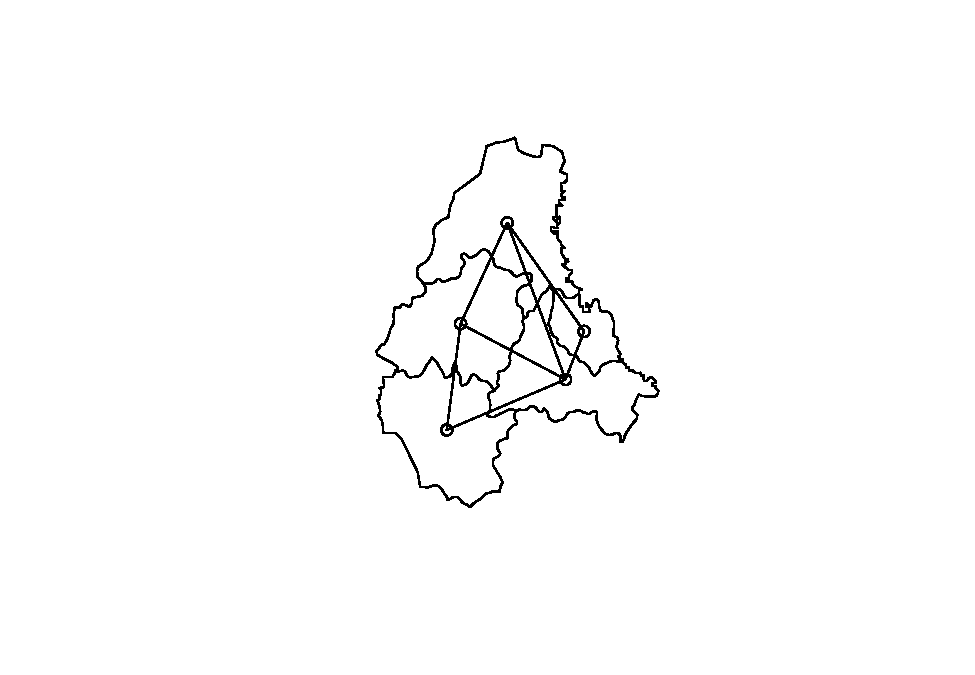
\includegraphics{modul_files/figure-latex/unnamed-chunk-32-1.pdf}

Jika yang ingin digunakan adalah kriteria \emph{rook contiguity}, maka kita dapat mengganti argumen pada program sebelumnya menjadi \texttt{queen=FALSE}.

\begin{Shaded}
\begin{Highlighting}[]
\NormalTok{w.rook }\OtherTok{\textless{}{-}} \FunctionTok{poly2nb}\NormalTok{(p, }\AttributeTok{queen=}\ConstantTok{FALSE}\NormalTok{)}
\NormalTok{coords}\OtherTok{\textless{}{-}}\FunctionTok{coordinates}\NormalTok{(p)}
\FunctionTok{plot}\NormalTok{(p)}
\FunctionTok{plot}\NormalTok{(w, coords, }\AttributeTok{add=}\NormalTok{T)}
\end{Highlighting}
\end{Shaded}

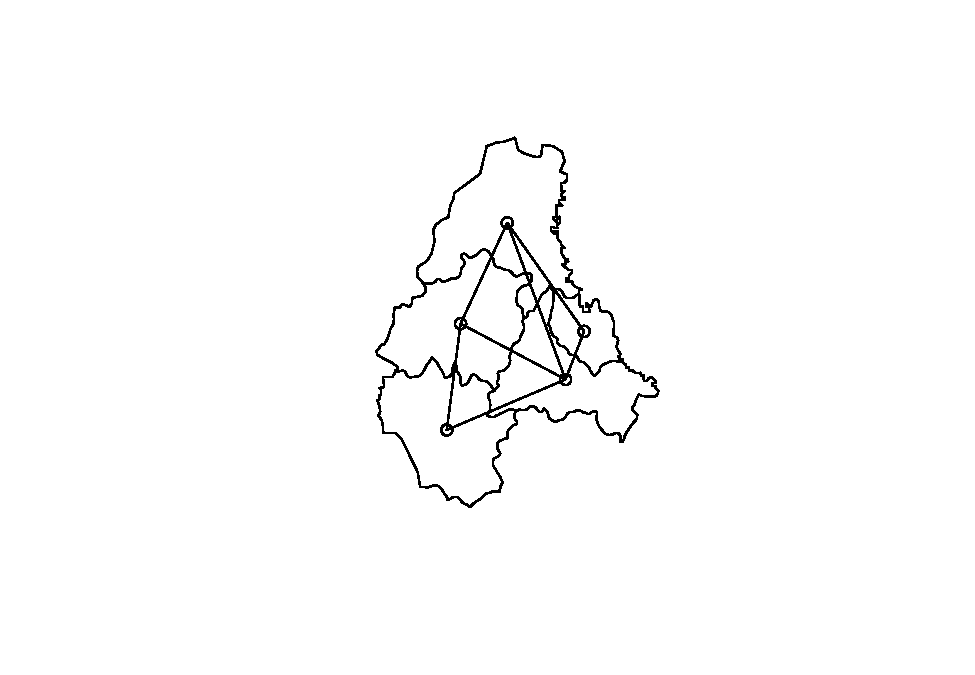
\includegraphics{modul_files/figure-latex/unnamed-chunk-33-1.pdf}

Perhatikan bahwa pada kasus ini, kedua kriteria memperlihatkan hasil yang sama. Hal ini terjadi karena semua area pada ilustrasi ini bersinggungan sudut.

\hypertarget{distance-based}{%
\subsubsection{\texorpdfstring{\emph{Distance Based}}{Distance Based}}\label{distance-based}}

Kriteria kebertetanggaan dapat pula ditentukan berdasarkan jarak antar lokasi, beberapa pendekatan jarak yang dapat digunakan adalah \(k\) tetangga terdekat (\emph{k nearest neighbours (KNN)}), \emph{radial distance}, \emph{power distance}, dan \emph{exponential distance}. Ilustrasi KNN dan \emph{radial distance} dapat dilihat pada subbab berikutnya dalam modul ini.

Pendekatan \emph{power distance} dan \emph{exponential distance} tidak diberikan ilustrasi pada modul ini, namun berikut adalah penjelasan singkat mengenai keduanya. Apabila bobot antara lokasi ke-\(i\) dan lokasi ke-\(j\) dinotasikan dengan \(w_{ij}\), dan jarak antara kedua lokasi tersebut dinotasikan dengan \(d_{ij}\), formula untuk memperoleh bobot jarak dengan pendekatan \emph{power distance} adalah:
\[
w_{ij}=d_{ij}^{-\alpha}
\]

Sedangkan bobot jarak berdasarkan \emph{exponential distance} dapat diperoleh dengan formula:
\[
w_{ij}=e^{{-\alpha}d_{ij}}
\]

\hypertarget{k-nearest-neighbours}{%
\paragraph{\texorpdfstring{\emph{K-Nearest Neighbours}}{K-Nearest Neighbours}}\label{k-nearest-neighbours}}

Pada pendekatan ini, kita mendefinisikan lokasi yang merupakan tetangga dari lokasi ke-\(i\) adalah sejumlah \(k\) lokasi yang memiliki jarak terdekat dengan lokasi \(i\).

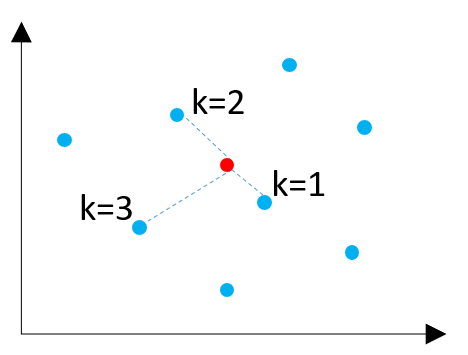
\includegraphics{D:/Research (eksternal dept)/pelatihan spasial (adj)/Modul Pelatihan Spasial/knn.png}

Berikut ini adalah ilustrasi untuk memperoleh ketetanggaan dengan pendekatan KNN menggunakan program R.

\begin{Shaded}
\begin{Highlighting}[]
\NormalTok{coords}\OtherTok{\textless{}{-}}\FunctionTok{coordinates}\NormalTok{(p)}
\NormalTok{IDs}\OtherTok{\textless{}{-}}\FunctionTok{row.names}\NormalTok{(}\FunctionTok{as}\NormalTok{(p, }\StringTok{"data.frame"}\NormalTok{))}
\NormalTok{p\_kn1}\OtherTok{\textless{}{-}}\FunctionTok{knn2nb}\NormalTok{(}\FunctionTok{knearneigh}\NormalTok{(coords, }\AttributeTok{k=}\DecValTok{1}\NormalTok{), }\AttributeTok{row.names=}\NormalTok{IDs)}
\NormalTok{p\_kn2}\OtherTok{\textless{}{-}}\FunctionTok{knn2nb}\NormalTok{(}\FunctionTok{knearneigh}\NormalTok{(coords, }\AttributeTok{k=}\DecValTok{2}\NormalTok{), }\AttributeTok{row.names=}\NormalTok{IDs)}
\NormalTok{p\_kn4}\OtherTok{\textless{}{-}}\FunctionTok{knn2nb}\NormalTok{(}\FunctionTok{knearneigh}\NormalTok{(coords, }\AttributeTok{k=}\DecValTok{4}\NormalTok{), }\AttributeTok{row.names=}\NormalTok{IDs)}

\FunctionTok{par}\NormalTok{(}\AttributeTok{mfrow=}\FunctionTok{c}\NormalTok{(}\DecValTok{1}\NormalTok{,}\DecValTok{3}\NormalTok{))}
\FunctionTok{plot}\NormalTok{(p, }\AttributeTok{main =} \StringTok{"k=1"}\NormalTok{)}
\FunctionTok{plot}\NormalTok{(p\_kn1, coords, }\AttributeTok{add=}\NormalTok{T)}

\FunctionTok{plot}\NormalTok{(p, }\AttributeTok{main =} \StringTok{"k=2"}\NormalTok{)}
\FunctionTok{plot}\NormalTok{(p\_kn2, coords, }\AttributeTok{add=}\NormalTok{T)}

\FunctionTok{plot}\NormalTok{(p, }\AttributeTok{main =} \StringTok{"k=4"}\NormalTok{)}
\FunctionTok{plot}\NormalTok{(p\_kn4, coords, }\AttributeTok{add=}\NormalTok{T)}
\end{Highlighting}
\end{Shaded}

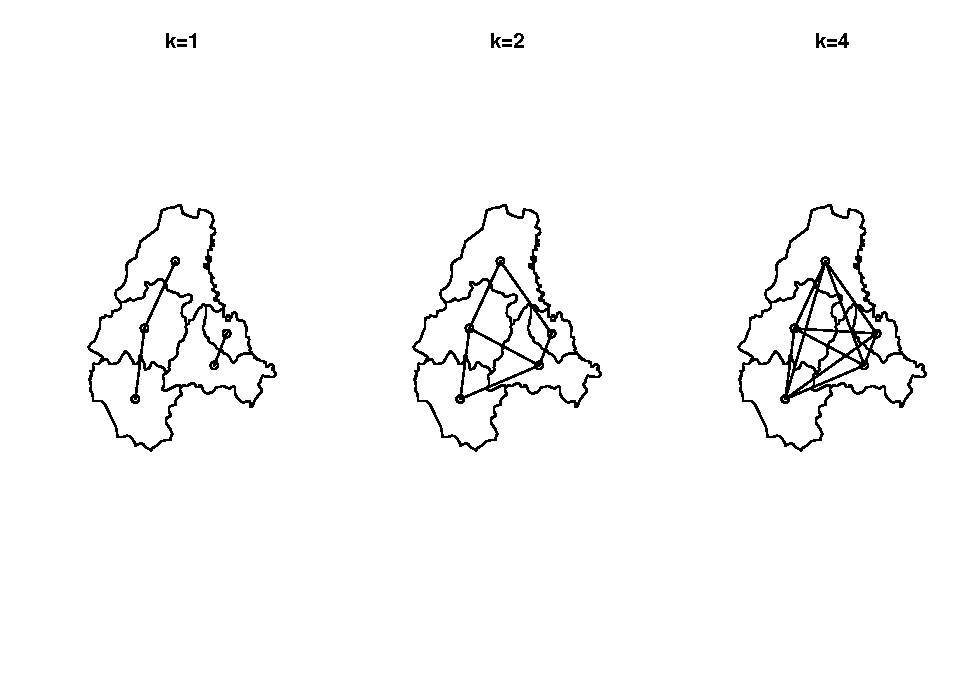
\includegraphics{modul_files/figure-latex/unnamed-chunk-34-1.pdf}

\hypertarget{radial-distance}{%
\paragraph{\texorpdfstring{\emph{Radial Distance}}{Radial Distance}}\label{radial-distance}}

Pada pendekatan ini,kita mendefinisikan lokasi yang merupakan tetangga dari lokasi ke-\(i\) adalah sejumlah \(k\) lokasi yang berada batas batas jarak (radius) antara \(d1\) dan \(d2\), diukur dari lokasi \(i\).

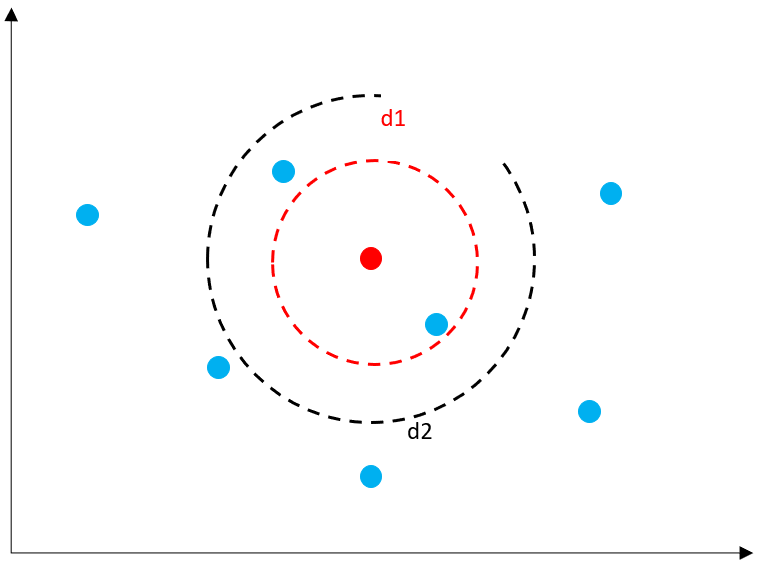
\includegraphics{D:/Research (eksternal dept)/pelatihan spasial (adj)/Modul Pelatihan Spasial/radial_distance.png}

Berikut ini adalah ilustrasi untuk memperoleh ketetanggaan dengan pendekatan KNN menggunakan program R.

\begin{Shaded}
\begin{Highlighting}[]
\NormalTok{dist}\OtherTok{\textless{}{-}}\FunctionTok{unlist}\NormalTok{(}\FunctionTok{nbdists}\NormalTok{(p\_kn1, coords))}
\FunctionTok{summary}\NormalTok{(dist)}
\end{Highlighting}
\end{Shaded}

\begin{verbatim}
##    Min. 1st Qu.  Median    Mean 3rd Qu.    Max. 
## 0.07316 0.07316 0.14159 0.11832 0.14159 0.16213
\end{verbatim}

\begin{Shaded}
\begin{Highlighting}[]
\FunctionTok{sort}\NormalTok{(dist)}
\end{Highlighting}
\end{Shaded}

\begin{verbatim}
## [1] 0.07315711 0.07315711 0.14158521 0.14158521 0.16213194
\end{verbatim}

\begin{Shaded}
\begin{Highlighting}[]
\NormalTok{max\_k1}\OtherTok{\textless{}{-}}\FunctionTok{max}\NormalTok{(dist)}
\NormalTok{p\_kd1}\OtherTok{\textless{}{-}}\FunctionTok{dnearneigh}\NormalTok{(coords, }\AttributeTok{d1=}\DecValTok{0}\NormalTok{, }\AttributeTok{d2=}\FloatTok{0.75}\SpecialCharTok{*}\NormalTok{max\_k1, }\AttributeTok{row.names=}\NormalTok{IDs)}
\NormalTok{p\_kd2}\OtherTok{\textless{}{-}}\FunctionTok{dnearneigh}\NormalTok{(coords, }\AttributeTok{d1=}\DecValTok{0}\NormalTok{, }\AttributeTok{d2=}\DecValTok{1}\SpecialCharTok{*}\NormalTok{max\_k1, }\AttributeTok{row.names=}\NormalTok{IDs)}
\NormalTok{p\_kd3}\OtherTok{\textless{}{-}}\FunctionTok{dnearneigh}\NormalTok{(coords, }\AttributeTok{d1=}\DecValTok{0}\NormalTok{, }\AttributeTok{d2=}\FloatTok{1.5}\SpecialCharTok{*}\NormalTok{max\_k1, }\AttributeTok{row.names=}\NormalTok{IDs)}

\FunctionTok{par}\NormalTok{(}\AttributeTok{mfrow=}\FunctionTok{c}\NormalTok{(}\DecValTok{1}\NormalTok{,}\DecValTok{3}\NormalTok{))}
\FunctionTok{plot}\NormalTok{(p, }\AttributeTok{main =} \StringTok{"Distance=0.75*max\_k1"}\NormalTok{)}
\FunctionTok{plot}\NormalTok{(p\_kd1,coords, }\AttributeTok{add=}\NormalTok{T)}

\FunctionTok{plot}\NormalTok{(p, }\AttributeTok{main =} \StringTok{"Distance=1*max\_k1"}\NormalTok{)}
\FunctionTok{plot}\NormalTok{(p\_kd2,coords, }\AttributeTok{add=}\NormalTok{T)}

\FunctionTok{plot}\NormalTok{(p, }\AttributeTok{main =} \StringTok{"Distance=1.5*max\_k1"}\NormalTok{)}
\FunctionTok{plot}\NormalTok{(p\_kd3,coords, }\AttributeTok{add=}\NormalTok{T)}
\end{Highlighting}
\end{Shaded}

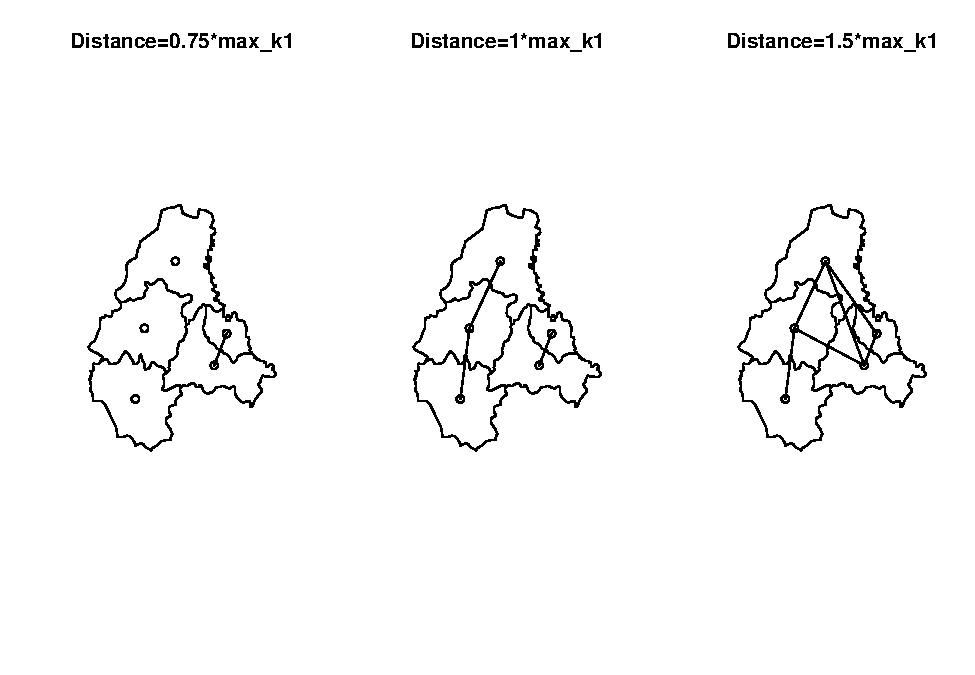
\includegraphics{modul_files/figure-latex/unnamed-chunk-35-1.pdf}

\hypertarget{matriks-pembobot-spasial}{%
\subsection{Matriks Pembobot Spasial}\label{matriks-pembobot-spasial}}

Matriks pembobot spasial dapat berisi elemen biner (1 atau 0) untuk menunjukkan ketetanggaan setiap lokasi, atau berupa matriks yang sudah distandardisasi. Umumnya, matriks pembobot spasial merupakan matriks yang terstandardisasi baris (\emph{row standardized}).

\begin{Shaded}
\begin{Highlighting}[]
\FunctionTok{nb2mat}\NormalTok{(w, }\AttributeTok{style=}\StringTok{"B"}\NormalTok{)  }\CommentTok{\#matriks pembobot biner}
\end{Highlighting}
\end{Shaded}

\begin{verbatim}
##   [,1] [,2] [,3] [,4] [,5]
## 0    0    1    0    1    1
## 1    1    0    1    1    1
## 2    0    1    0    0    1
## 3    1    1    0    0    0
## 4    1    1    1    0    0
## attr(,"call")
## nb2mat(neighbours = w, style = "B")
\end{verbatim}

\begin{Shaded}
\begin{Highlighting}[]
\FunctionTok{nb2mat}\NormalTok{(w) }\CommentTok{\# matriks pembobot row standardized}
\end{Highlighting}
\end{Shaded}

\begin{verbatim}
##        [,1]      [,2]      [,3]      [,4]      [,5]
## 0 0.0000000 0.3333333 0.0000000 0.3333333 0.3333333
## 1 0.2500000 0.0000000 0.2500000 0.2500000 0.2500000
## 2 0.0000000 0.5000000 0.0000000 0.0000000 0.5000000
## 3 0.5000000 0.5000000 0.0000000 0.0000000 0.0000000
## 4 0.3333333 0.3333333 0.3333333 0.0000000 0.0000000
## attr(,"call")
## nb2mat(neighbours = w)
\end{verbatim}

\hypertarget{autokorelasi-spasial}{%
\subsection{Autokorelasi Spasial}\label{autokorelasi-spasial}}

\hypertarget{indeks-moran-global}{%
\subsubsection{Indeks Moran Global}\label{indeks-moran-global}}

Sebagai ilustrasi, akan digunakan data persentase kemiskinan kabupaten/kota di Pulau Jawa. Berikut adalah syntax untuk membaca peta Pulau Jawa dan data persentase kemiskinan Kabupaten/Kota di Pulau Jawa

\begin{Shaded}
\begin{Highlighting}[]
\FunctionTok{library}\NormalTok{(rgdal)}
\FunctionTok{library}\NormalTok{(spdep)}
\FunctionTok{library}\NormalTok{(sp)}
\NormalTok{petajawa}\OtherTok{=}\FunctionTok{readOGR}\NormalTok{(}\AttributeTok{dsn=}\StringTok{"Jawamap"}\NormalTok{, }\AttributeTok{layer=}\StringTok{"jawa"}\NormalTok{)}
\end{Highlighting}
\end{Shaded}

\begin{verbatim}
## OGR data source with driver: ESRI Shapefile 
## Source: "D:\Jobs\Pelatihan Spasial STIS\New folder\Pelatihan-Spasial\Jawamap", layer: "jawa"
## with 119 features
## It has 5 fields
\end{verbatim}

\begin{Shaded}
\begin{Highlighting}[]
\NormalTok{datajawa}\OtherTok{=}\FunctionTok{read.csv}\NormalTok{(}\StringTok{"Pulau Jawa.csv"}\NormalTok{, }\AttributeTok{header=}\NormalTok{T, }\AttributeTok{sep=}\StringTok{";"}\NormalTok{)}
\NormalTok{petajawa}\SpecialCharTok{$}\NormalTok{Kemiskinan}\OtherTok{\textless{}{-}}\NormalTok{ datajawa}\SpecialCharTok{$}\NormalTok{Kemiskinan}
\NormalTok{k}\OtherTok{=}\DecValTok{9}
\NormalTok{colfunc }\OtherTok{\textless{}{-}} \FunctionTok{colorRampPalette}\NormalTok{(}\FunctionTok{c}\NormalTok{(}\StringTok{"green"}\NormalTok{, }\StringTok{"yellow"}\NormalTok{,}\StringTok{"red"}\NormalTok{))}
\NormalTok{color }\OtherTok{\textless{}{-}} \FunctionTok{colfunc}\NormalTok{(k)}
\FunctionTok{spplot}\NormalTok{(petajawa, }\StringTok{"Kemiskinan"}\NormalTok{, }\AttributeTok{col.regions=}\NormalTok{color)}
\end{Highlighting}
\end{Shaded}

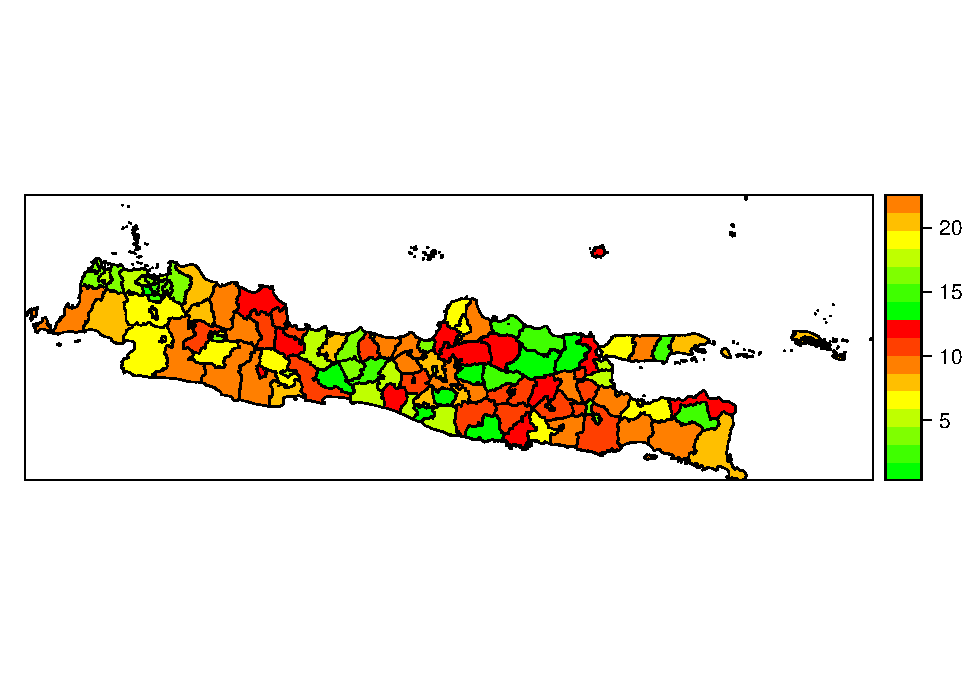
\includegraphics{modul_files/figure-latex/unnamed-chunk-38-1.pdf}

Seandainya kita akan menggunakan kriteria queen contiguity, maka dapat dilakukan dengan syntax berikut untuk mendefinisikan matriks pembobotnya

\begin{Shaded}
\begin{Highlighting}[]
\NormalTok{w.queen }\OtherTok{\textless{}{-}} \FunctionTok{poly2nb}\NormalTok{(petajawa)}
\NormalTok{w.queen}
\end{Highlighting}
\end{Shaded}

\begin{verbatim}
## Neighbour list object:
## Number of regions: 119 
## Number of nonzero links: 522 
## Percentage nonzero weights: 3.68618 
## Average number of links: 4.386555 
## 1 region with no links:
## 0
\end{verbatim}

Terlihat pada output tersebut, bahwa terdapat 1 wilayah yang tidak memiliki tetangga, sehingga untuk syntax selanjutnya perlu ditambahkan \texttt{zero.policy=T}.

\begin{Shaded}
\begin{Highlighting}[]
\NormalTok{wqueen }\OtherTok{\textless{}{-}} \FunctionTok{nb2listw}\NormalTok{(w.queen, }\AttributeTok{zero.policy=}\NormalTok{T)}
\end{Highlighting}
\end{Shaded}

Seandainya kita ingin menguji autokorelasi menggunakan pendekatan indeks moran, maka kita dapat menggunakan fungsi \texttt{moran.test()}.

\begin{Shaded}
\begin{Highlighting}[]
\NormalTok{I1 }\OtherTok{\textless{}{-}} \FunctionTok{moran.test}\NormalTok{(petajawa}\SpecialCharTok{$}\NormalTok{Kemiskinan, wqueen, }\AttributeTok{zero.policy=}\NormalTok{T, }\AttributeTok{alternative=}\StringTok{"greater"}\NormalTok{)}

\CommentTok{\#alternative hyptohesis could be either of "two.sided", "greater", or "less"}

\NormalTok{I1}
\end{Highlighting}
\end{Shaded}

\begin{verbatim}
## 
##  Moran I test under randomisation
## 
## data:  petajawa$Kemiskinan  
## weights: wqueen  n reduced by no-neighbour observations
##   
## 
## Moran I statistic standard deviate = 7.7638, p-value = 4.12e-15
## alternative hypothesis: greater
## sample estimates:
## Moran I statistic       Expectation          Variance 
##       0.517060772      -0.008547009       0.004583226
\end{verbatim}

Berdasarkan output di atas, diperoleh nilai p-value yang sangat kecil, artinya kita dapat menolak hipotesis nol yang menyatakan bahwa tidak terdapat autokorelasi.Artinya kita dapat menyimpulkan bahwa terdapat cukup bukti untuk menyatakan bahwa terdapat autokorelasi pada taraf nyata 5\%.

Uji moran dapat pula dilakukan dengan melibatkan simulasi monte carlo.

\begin{Shaded}
\begin{Highlighting}[]
\FunctionTok{set.seed}\NormalTok{(}\DecValTok{123}\NormalTok{)}
\NormalTok{MC}\OtherTok{\textless{}{-}} \FunctionTok{moran.mc}\NormalTok{(petajawa}\SpecialCharTok{$}\NormalTok{Kemiskinan, wqueen, }\AttributeTok{nsim=}\DecValTok{99}\NormalTok{, }\AttributeTok{zero.policy=}\NormalTok{T, }\AttributeTok{alternative=}\StringTok{"greater"}\NormalTok{)}

\CommentTok{\# View results (including p{-}value)}
\NormalTok{MC}
\end{Highlighting}
\end{Shaded}

\begin{verbatim}
## 
##  Monte-Carlo simulation of Moran I
## 
## data:  petajawa$Kemiskinan 
## weights: wqueen  
## number of simulations + 1: 100 
## 
## statistic = 0.51706, observed rank = 100, p-value = 0.01
## alternative hypothesis: greater
\end{verbatim}

\hypertarget{indeks-moran-lokal}{%
\subsubsection{Indeks Moran Lokal}\label{indeks-moran-lokal}}

Pendekatan ini termasuk ke dalam \emph{Local Indicators for Spatial Association (LISA)}, yang mengindentifikasi autokorelasi pada tingkat lokal.

\begin{Shaded}
\begin{Highlighting}[]
\NormalTok{oid }\OtherTok{\textless{}{-}} \FunctionTok{order}\NormalTok{(petajawa}\SpecialCharTok{$}\NormalTok{Kemiskinan)}
\NormalTok{resI }\OtherTok{\textless{}{-}} \FunctionTok{localmoran}\NormalTok{(petajawa}\SpecialCharTok{$}\NormalTok{Kemiskinan, wqueen)}
\end{Highlighting}
\end{Shaded}

\begin{verbatim}
## Warning in lag.listw(listw, z, zero.policy = zero.policy, NAOK = NAOK): NAs in
## lagged values
\end{verbatim}

\begin{Shaded}
\begin{Highlighting}[]
\FunctionTok{head}\NormalTok{(resI)}
\end{Highlighting}
\end{Shaded}

\begin{verbatim}
##         Ii         E.Ii    Var.Ii     Z.Ii    Pr(z > 0)
## 0       NA  0.000000000 0.0000000       NA           NA
## 1 2.514160 -0.008474576 0.1571389 6.363741 9.844878e-11
## 2 2.172630 -0.008474576 0.1571389 5.502177 1.875645e-08
## 3 2.040414 -0.008474576 0.2398473 4.183607 1.434598e-05
## 4 1.872452 -0.008474576 0.1902223 4.312619 8.066594e-06
## 5 1.382831 -0.008474576 0.1902223 3.190008 7.113445e-04
\end{verbatim}

\begin{Shaded}
\begin{Highlighting}[]
\NormalTok{petajawa}\SpecialCharTok{$}\NormalTok{z.li }\OtherTok{\textless{}{-}}\NormalTok{ resI[,}\DecValTok{4}\NormalTok{]}
\NormalTok{petajawa}\SpecialCharTok{$}\NormalTok{pvalue }\OtherTok{\textless{}{-}}\NormalTok{ resI[,}\DecValTok{5}\NormalTok{]}
\NormalTok{lm.palette }\OtherTok{\textless{}{-}} \FunctionTok{colorRampPalette}\NormalTok{(}\FunctionTok{c}\NormalTok{(}\StringTok{"white"}\NormalTok{,}\StringTok{"orange"}\NormalTok{, }\StringTok{"red"}\NormalTok{), }\AttributeTok{space =} \StringTok{"rgb"}\NormalTok{)}
\FunctionTok{spplot}\NormalTok{(petajawa, }\AttributeTok{zcol=}\StringTok{"z.li"}\NormalTok{, }\AttributeTok{col.regions=}\FunctionTok{lm.palette}\NormalTok{(}\DecValTok{20}\NormalTok{), }\AttributeTok{main=}\StringTok{"Local Moran"}\NormalTok{)}
\end{Highlighting}
\end{Shaded}

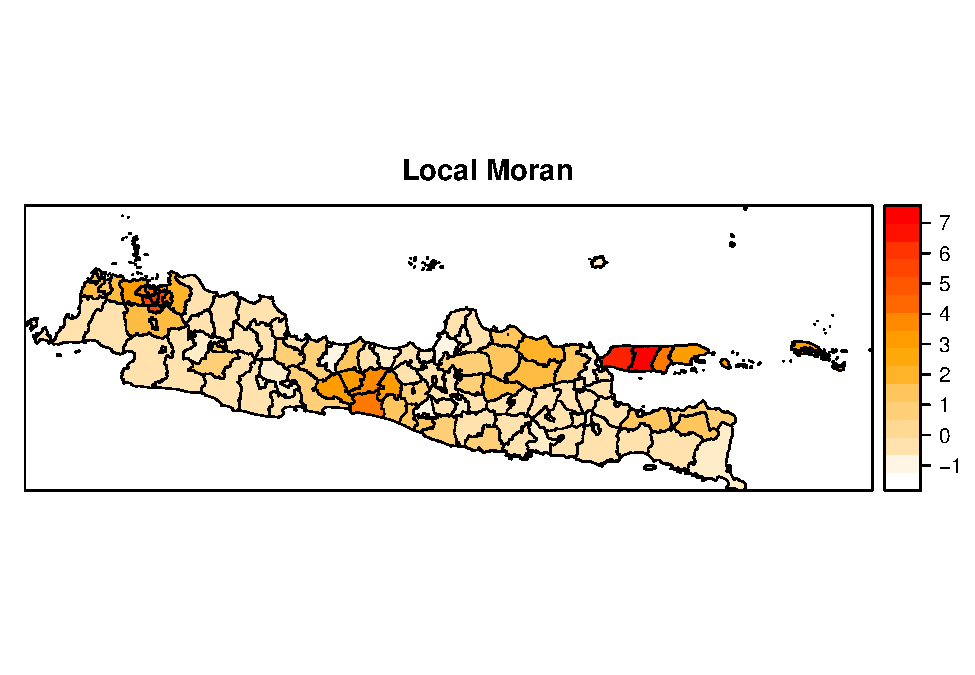
\includegraphics{modul_files/figure-latex/unnamed-chunk-44-1.pdf}

\begin{Shaded}
\begin{Highlighting}[]
\FunctionTok{moran.plot}\NormalTok{(petajawa}\SpecialCharTok{$}\NormalTok{Kemiskinan, wqueen, }\AttributeTok{zero.policy=}\NormalTok{T, }\AttributeTok{labels=}\NormalTok{petajawa}\SpecialCharTok{$}\NormalTok{KABKOT)}
\end{Highlighting}
\end{Shaded}

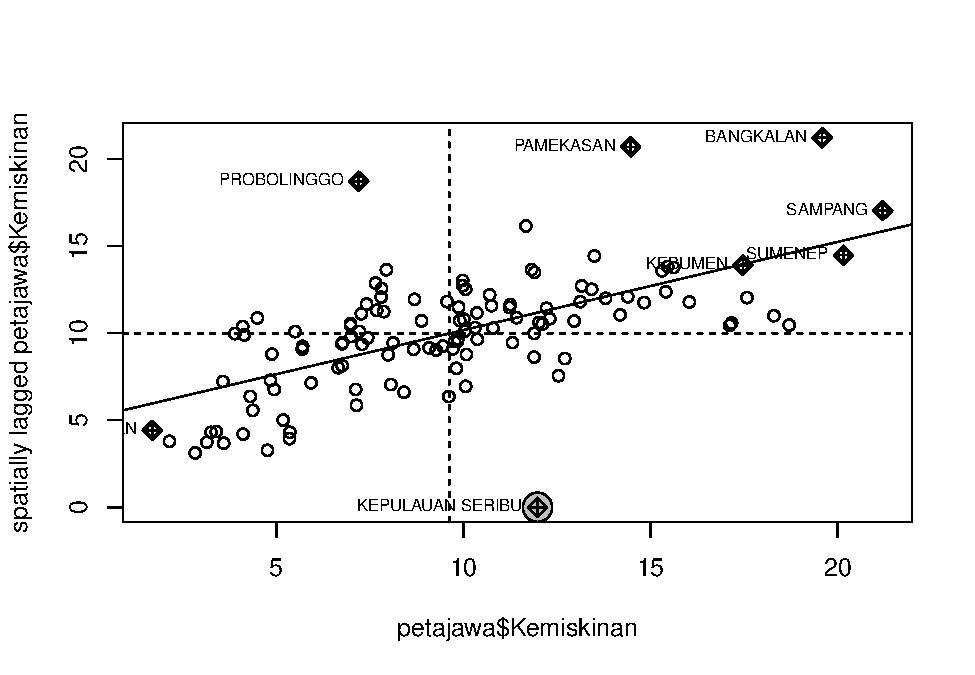
\includegraphics{modul_files/figure-latex/unnamed-chunk-45-1.pdf}

\hypertarget{sumber-pustaka}{%
\section{Sumber Pustaka}\label{sumber-pustaka}}

Agafonkin, V. (n.d.). Leaflet for R - Markers. rstudio.github.io. Retrieved from \url{https://rstudio.github.io/leaflet/markers.html}

Baumer, B.S., Kaplan, D.T., Horton, N.J. 2017. Modern Data Science with R. CRC Press.

UQ SLC Digital Team. (2020, April 16). Creating maps using R. Language Technology and Data Analysis Laboratory (LADAL). Retrieved from \url{https://slcladal.github.io/maps.html}

\hypertarget{pemodelan-dependensi-spasial}{%
\chapter{Pemodelan Dependensi Spasial}\label{pemodelan-dependensi-spasial}}

\hypertarget{model-spasial-global}{%
\section{Model Spasial Global}\label{model-spasial-global}}

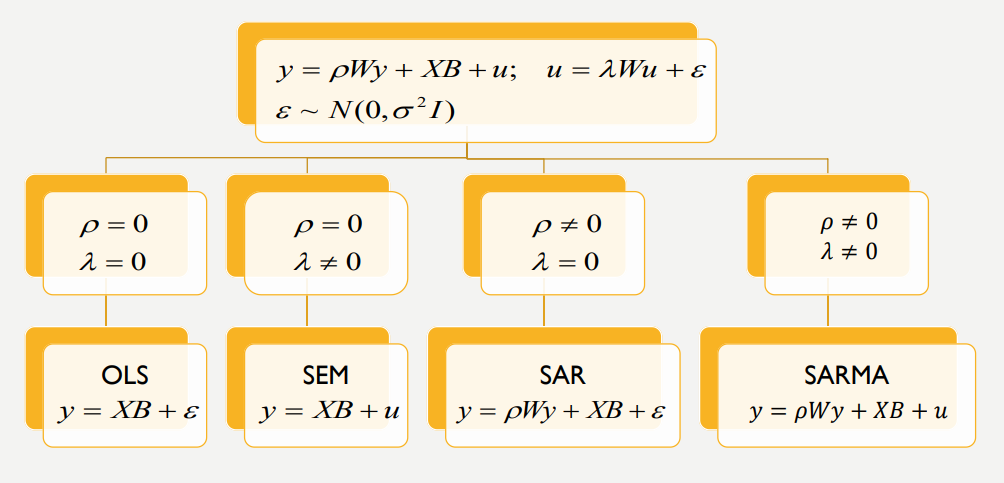
\includegraphics{D:/Research (eksternal dept)/pelatihan spasial (adj)/Modul Pelatihan Spasial/gambar 2.PNG}

Secara umum, tahapan pemodelan regresi spasial adalah sebagai berikut:

\begin{enumerate}
\def\labelenumi{(\arabic{enumi})}
\item
  Eksplorasi Data
\item
  Regresi Klasik \& Uji Asumsi
\item
  Matriks Pembobot Spasial
\item
  Uji Lagrange Multiplier
\item
  Regresi Spasial \& Uji Asumsi
\item
  Kebaikan Model
\end{enumerate}

Sebagai ilustrasi untuk menjelaskan tahapan tersebut, kita akan menggunakan data kemiskinan dan kependudukan di Pulau Jawa berikut ini:

\begin{enumerate}
\def\labelenumi{\arabic{enumi}.}
\item
  Data polygon (peta Pulau Jawa, dengan extension .shp)
\item
  Data frame (data persentase kemiskinan, PDRB, pendidikan Angka Melek Huruf, Pengeluaran perkapita, Ruta Penerima Raskin, Penduduk berusia 15-64, Harapan Lama Sekolah, dan Rata-Rata Lama Sekolah, diperoleh dari BPS)
\end{enumerate}

Seperti yang telah dijelaskan pada modul sebelumnya, impor data dapat dilakukan dengan program berikut ini.

\begin{Shaded}
\begin{Highlighting}[]
\NormalTok{datajawa }\OtherTok{=}\NormalTok{ datajawa}\OtherTok{=}\FunctionTok{read.csv}\NormalTok{(}\StringTok{"Pulau Jawa.csv"}\NormalTok{, }\AttributeTok{header=}\NormalTok{T, }\AttributeTok{sep=}\StringTok{";"}\NormalTok{)}
\FunctionTok{head}\NormalTok{(datajawa)}
\end{Highlighting}
\end{Shaded}

\begin{verbatim}
##      Provinsi       Kabupaten.kota Longitude Latitude Kemiskinan   PDRB
## 1 DKI Jakarta     Kepulauan Seribu  106.5072  -5.7985      11.98 338.80
## 2             Kota Jakarta Selatan  106.8079  -6.2627       2.83 261.58
## 3               Kota Jakarta Timur  106.8995  -6.2249       3.14 155.53
## 4               Kota Jakarta Pusat  106.8279  -6.1801       3.59 692.24
## 5               Kota Jakarta Barat  106.7633  -6.1675       3.39 168.68
## 6               Kota Jakarta Utara  106.8926  -6.1555       5.35 271.85
##   Pendidikan    AMH Pengeluaran.Perkapita Ruta.Penerima.Raskin Penduduk.15.64
## 1       5.29 100.00                 68.80                55.34        86.2882
## 2       7.96 100.00                 46.63                 0.00        86.8031
## 3       2.91 100.00                 50.39                 0.00        86.9343
## 4       3.62 100.00                 50.87                 0.00        86.2032
## 5      25.02 100.00                 53.29                 0.00        87.4070
## 6      18.59  98.98                 51.12                 0.00        87.3943
##     HLS Rata.Rata.Lama.Sekolah
## 1 12.48                   8.46
## 2 13.31                  11.57
## 3 13.43                  11.64
## 4 13.23                  11.24
## 5 12.78                  10.38
## 6 12.61                  10.69
\end{verbatim}

Pada ilustrasi ini, pemodelan dilakukan untuk mengkaji peubah respon \textbf{persentase penduduk miskin tahun 2018 di pulau Jawa (\(Y\))} dengan menggunakan peubah \textbf{persentase Pendidikan yang ditamatkan di Bawah SD Tahun 2018(\(X\))}.

\begin{Shaded}
\begin{Highlighting}[]
\FunctionTok{library}\NormalTok{(spdep)}
\FunctionTok{library}\NormalTok{(rgdal)}
\FunctionTok{library}\NormalTok{(raster)}

\NormalTok{petajawa}\OtherTok{\textless{}{-}}\FunctionTok{readOGR}\NormalTok{(}\AttributeTok{dsn=}\NormalTok{“directory tempat folder utk file .shp}\StringTok{", layer=“nama file shp"}\NormalTok{)}
\end{Highlighting}
\end{Shaded}

\hypertarget{eksplorasi-data}{%
\section{Eksplorasi Data}\label{eksplorasi-data}}

\begin{Shaded}
\begin{Highlighting}[]
\FunctionTok{hist}\NormalTok{(datajawa}\SpecialCharTok{$}\NormalTok{Kemiskinan)}
\end{Highlighting}
\end{Shaded}

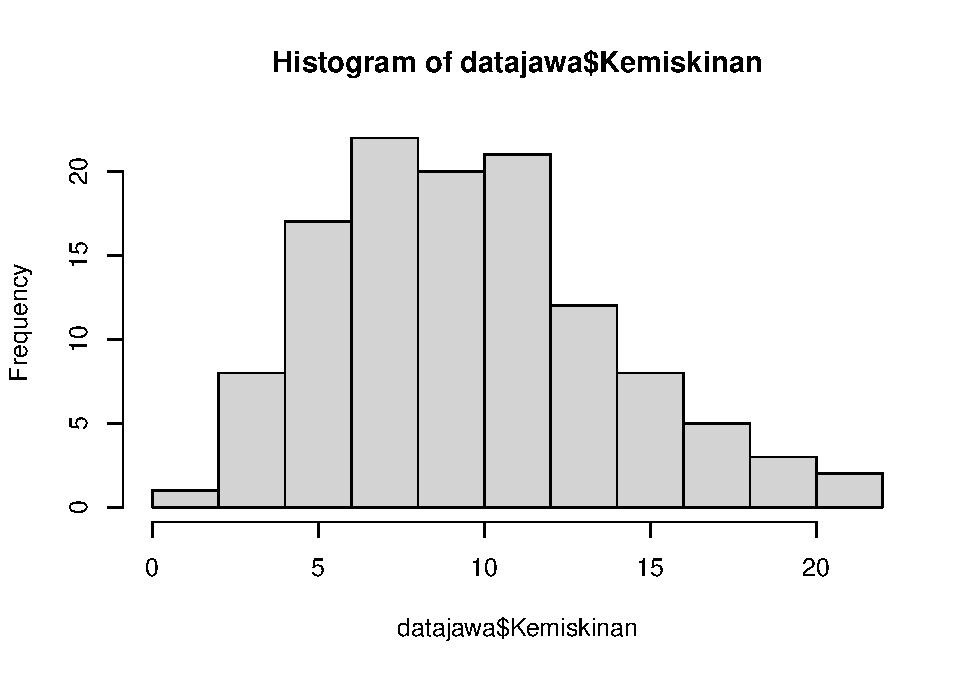
\includegraphics{modul_files/figure-latex/unnamed-chunk-49-1.pdf}

\begin{Shaded}
\begin{Highlighting}[]
\NormalTok{bxplt}\OtherTok{\textless{}{-}}\FunctionTok{boxplot}\NormalTok{(datajawa}\SpecialCharTok{$}\NormalTok{Kemiskinan, }\AttributeTok{outlier.tagging=}\NormalTok{T)}
\end{Highlighting}
\end{Shaded}

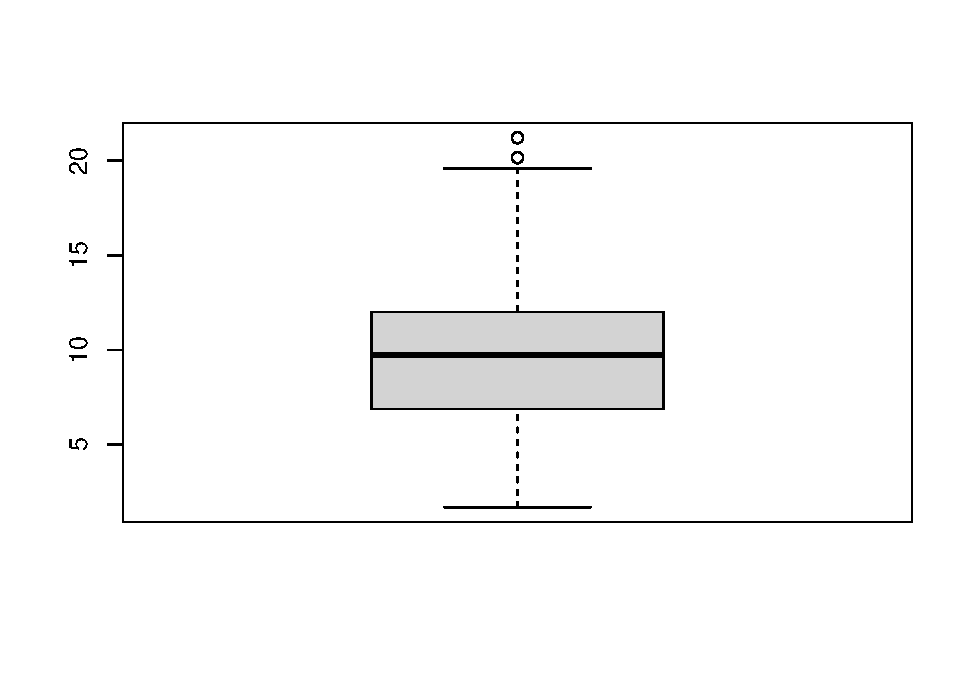
\includegraphics{modul_files/figure-latex/unnamed-chunk-50-1.pdf}

\begin{Shaded}
\begin{Highlighting}[]
\NormalTok{bxplt}\SpecialCharTok{$}\NormalTok{out}
\end{Highlighting}
\end{Shaded}

\begin{verbatim}
## [1] 21.21 20.16
\end{verbatim}

\begin{Shaded}
\begin{Highlighting}[]
\FunctionTok{subset}\NormalTok{(datajawa, datajawa}\SpecialCharTok{$}\NormalTok{Kemiskinan}\SpecialCharTok{\textgreater{}}\NormalTok{bxplt}\SpecialCharTok{$}\NormalTok{stats[}\DecValTok{5}\NormalTok{])}
\end{Highlighting}
\end{Shaded}

\begin{verbatim}
##     Provinsi Kabupaten.kota Longitude Latitude Kemiskinan  PDRB Pendidikan
## 100                 Sampang  113.2394  -7.0402      21.21 19.85      50.59
## 102                 Sumenep  113.9061  -6.9254      20.16 30.17      49.17
##       AMH Pengeluaran.Perkapita Ruta.Penerima.Raskin Penduduk.15.64   HLS
## 100 88.94                 69.82                67.89        66.5778 11.76
## 102 85.90                 64.05                78.71        71.6376 13.07
##     Rata.Rata.Lama.Sekolah
## 100                   4.36
## 102                   5.23
\end{verbatim}

\begin{Shaded}
\begin{Highlighting}[]
\FunctionTok{plot}\NormalTok{(datajawa}\SpecialCharTok{$}\NormalTok{Pendidikan, datajawa}\SpecialCharTok{$}\NormalTok{Kemiskinan,}
  \AttributeTok{xlab=}\StringTok{"Persentase Pendidikan yang ditamatkan di bawah SD Thn.2018"}\NormalTok{, }
  \AttributeTok{ylab=}\StringTok{"Persentase Penduduk Miskin Thn.2018"}\NormalTok{,}
  \AttributeTok{pch=}\DecValTok{20}\NormalTok{, }\AttributeTok{col=}\StringTok{"orange"}\NormalTok{, }\AttributeTok{cex=}\DecValTok{2}\NormalTok{)}
\end{Highlighting}
\end{Shaded}

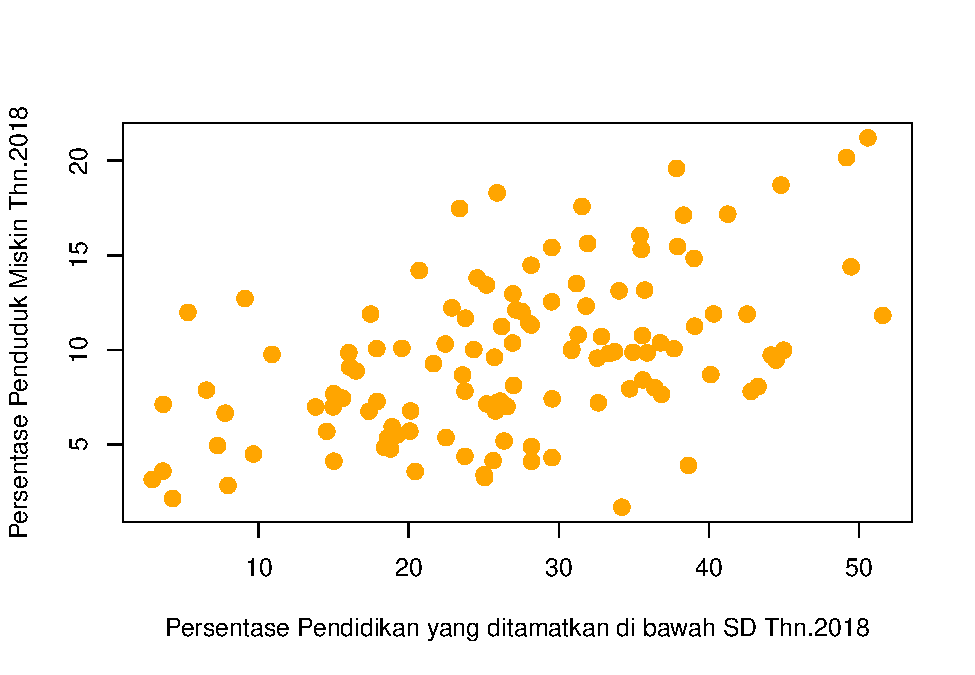
\includegraphics{modul_files/figure-latex/unnamed-chunk-51-1.pdf}

Plot tersebut memperlihatkan adanya pola hubungan linear positif antara persentase pendidikan yang ditamatkan di bawah SD terhadap persentase penduduk miskin di Pulau Jawa pada tahun 2018.

\begin{Shaded}
\begin{Highlighting}[]
\NormalTok{petajawa}\SpecialCharTok{$}\NormalTok{Kemiskinan}\OtherTok{\textless{}{-}}\NormalTok{ datajawa}\SpecialCharTok{$}\NormalTok{Kemiskinan}
\NormalTok{k}\OtherTok{=}\DecValTok{16}
\NormalTok{colfunc }\OtherTok{\textless{}{-}} \FunctionTok{colorRampPalette}\NormalTok{(}\FunctionTok{c}\NormalTok{(}\StringTok{"green"}\NormalTok{, }\StringTok{"yellow"}\NormalTok{,}\StringTok{"red"}\NormalTok{))}
\NormalTok{color }\OtherTok{\textless{}{-}} \FunctionTok{colfunc}\NormalTok{(k)}
\FunctionTok{spplot}\NormalTok{(petajawa, }\StringTok{"Kemiskinan"}\NormalTok{, }\AttributeTok{col.regions=}\NormalTok{color, }\AttributeTok{main=}\StringTok{"Persentase Penduduk Miskin Tahun 2018"}\NormalTok{)}
\end{Highlighting}
\end{Shaded}

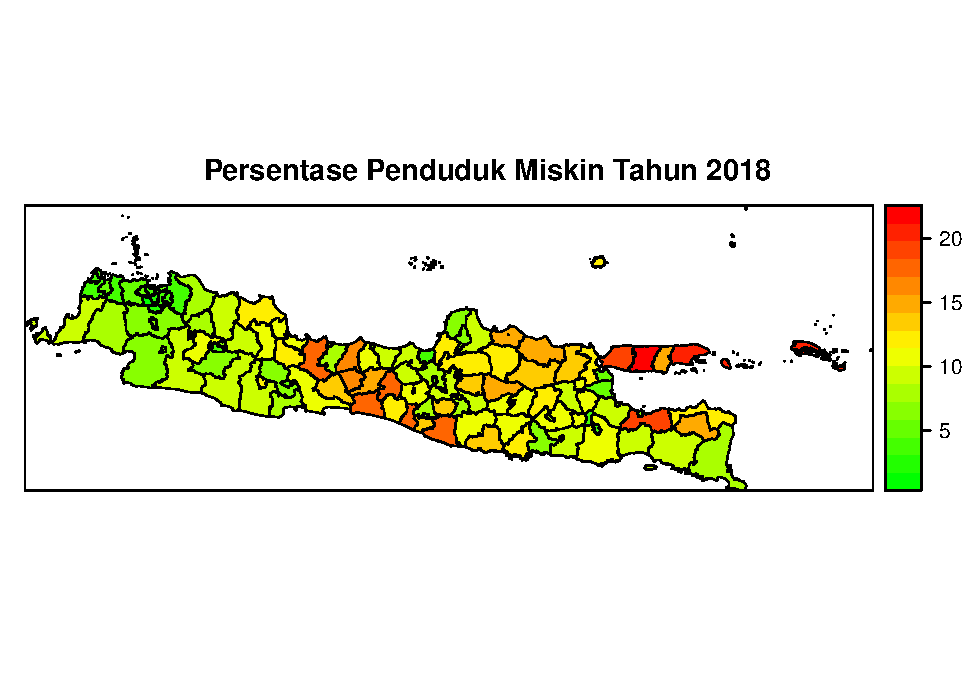
\includegraphics{modul_files/figure-latex/unnamed-chunk-52-1.pdf}

Berdasarkan plot di atas, dapat dilihat adanya kecenderungan pola bergerombol pada data persentase kemiskinan di kabupaten/kota di Pulau Jawa. Hal ini tampak dari gradasi warna yang cenderung mengumpul, seperti pada warna hijau, merah dan oranye.

\hypertarget{identifikasi-autokorelasi-pada-data}{%
\subsection{Identifikasi Autokorelasi pada Data}\label{identifikasi-autokorelasi-pada-data}}

\begin{Shaded}
\begin{Highlighting}[]
\NormalTok{w}\OtherTok{\textless{}{-}}\FunctionTok{poly2nb}\NormalTok{(petajawa)}
\NormalTok{ww}\OtherTok{\textless{}{-}}\FunctionTok{nb2listw}\NormalTok{(w, }\AttributeTok{zero.policy=}\NormalTok{T)}
\FunctionTok{moran}\NormalTok{(datajawa}\SpecialCharTok{$}\NormalTok{Kemiskinan, ww, }\AttributeTok{n=}\FunctionTok{length}\NormalTok{(ww}\SpecialCharTok{$}\NormalTok{neighbours), }
      \AttributeTok{S0=}\FunctionTok{Szero}\NormalTok{(ww), }\AttributeTok{zero.policy=}\NormalTok{T)}
\end{Highlighting}
\end{Shaded}

\begin{verbatim}
## $I
## [1] 0.5214426
## 
## $K
## [1] 2.853193
\end{verbatim}

\begin{Shaded}
\begin{Highlighting}[]
\FunctionTok{moran.test}\NormalTok{(datajawa}\SpecialCharTok{$}\NormalTok{Kemiskinan, ww,}\AttributeTok{randomisation=}\NormalTok{T, }
           \AttributeTok{alternative=}\StringTok{"greater"}\NormalTok{, }\AttributeTok{zero.policy=}\NormalTok{T)}
\end{Highlighting}
\end{Shaded}

\begin{verbatim}
## 
##  Moran I test under randomisation
## 
## data:  datajawa$Kemiskinan  
## weights: ww  n reduced by no-neighbour observations
##   
## 
## Moran I statistic standard deviate = 7.7638, p-value = 4.12e-15
## alternative hypothesis: greater
## sample estimates:
## Moran I statistic       Expectation          Variance 
##       0.517060772      -0.008547009       0.004583226
\end{verbatim}

\begin{Shaded}
\begin{Highlighting}[]
\FunctionTok{moran.plot}\NormalTok{(datajawa}\SpecialCharTok{$}\NormalTok{Kemiskinan, ww, }\AttributeTok{labels=}\NormalTok{petajawa}\SpecialCharTok{$}\NormalTok{KABKOT, }\AttributeTok{zero.policy=}\NormalTok{T)}
\end{Highlighting}
\end{Shaded}

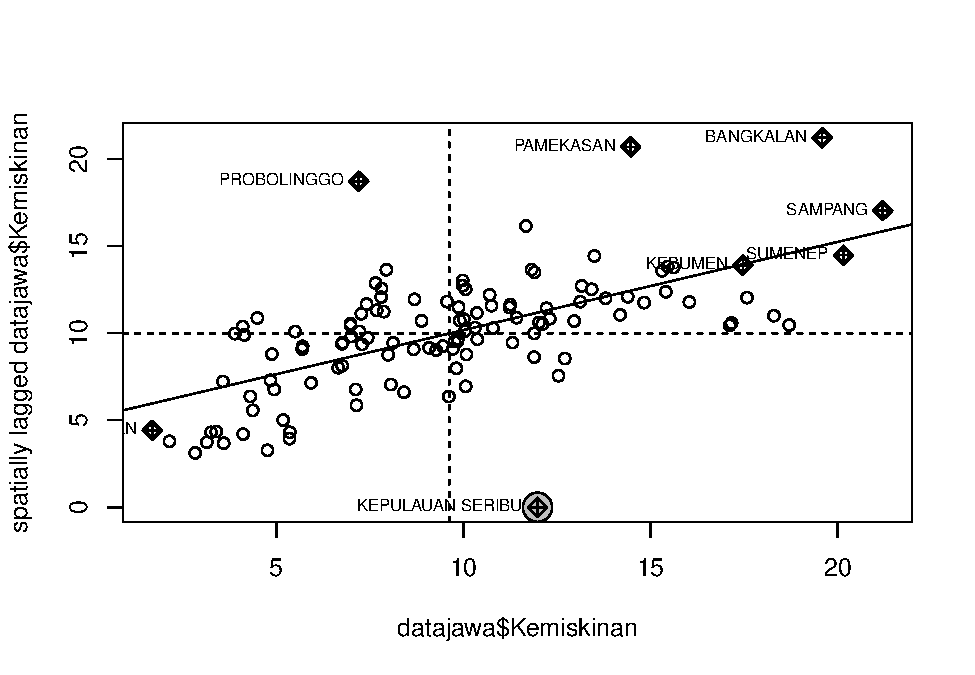
\includegraphics{modul_files/figure-latex/unnamed-chunk-54-1.pdf}

\hypertarget{pemodelan-regresi-klasik}{%
\section{Pemodelan Regresi Klasik}\label{pemodelan-regresi-klasik}}

Pemodelan regresi dapat dilakukan menggunakan fungsi \texttt{lm} berikut.

\begin{Shaded}
\begin{Highlighting}[]
\NormalTok{reg.klasik }\OtherTok{=} \FunctionTok{lm}\NormalTok{(Kemiskinan}\SpecialCharTok{\textasciitilde{}}\NormalTok{Pendidikan, }\AttributeTok{data =}\NormalTok{ datajawa)}
\NormalTok{err.regklasik}\OtherTok{\textless{}{-}}\FunctionTok{residuals}\NormalTok{(reg.klasik)}
\FunctionTok{summary}\NormalTok{(reg.klasik)}
\end{Highlighting}
\end{Shaded}

\begin{verbatim}
## 
## Call:
## lm(formula = Kemiskinan ~ Pendidikan, data = datajawa)
## 
## Residuals:
##     Min      1Q  Median      3Q     Max 
## -9.3117 -2.6659 -0.3763  2.2998  8.8844 
## 
## Coefficients:
##             Estimate Std. Error t value Pr(>|t|)    
## (Intercept)  4.50549    0.89314   5.045 1.68e-06 ***
## Pendidikan   0.18965    0.03066   6.186 9.37e-09 ***
## ---
## Signif. codes:  0 '***' 0.001 '**' 0.01 '*' 0.05 '.' 0.1 ' ' 1
## 
## Residual standard error: 3.671 on 117 degrees of freedom
## Multiple R-squared:  0.2464, Adjusted R-squared:   0.24 
## F-statistic: 38.26 on 1 and 117 DF,  p-value: 9.373e-09
\end{verbatim}

\begin{Shaded}
\begin{Highlighting}[]
\FunctionTok{cor}\NormalTok{(datajawa}\SpecialCharTok{$}\NormalTok{Kemiskinan, }\FunctionTok{fitted}\NormalTok{(reg.klasik))}\SpecialCharTok{\^{}}\DecValTok{2}
\end{Highlighting}
\end{Shaded}

\begin{verbatim}
## [1] 0.2464408
\end{verbatim}

\hypertarget{diagnostik-model}{%
\section{Diagnostik Model}\label{diagnostik-model}}

\hypertarget{kenormalan-sisaan}{%
\subsection{Kenormalan Sisaan}\label{kenormalan-sisaan}}

\begin{Shaded}
\begin{Highlighting}[]
\FunctionTok{library}\NormalTok{(nortest)}
\FunctionTok{library}\NormalTok{(car)}
\FunctionTok{library}\NormalTok{(DescTools)}
\FunctionTok{library}\NormalTok{(lmtest)}
\FunctionTok{shapiro.test}\NormalTok{(err.regklasik)}
\end{Highlighting}
\end{Shaded}

\begin{verbatim}
## 
##  Shapiro-Wilk normality test
## 
## data:  err.regklasik
## W = 0.98607, p-value = 0.2608
\end{verbatim}

\begin{Shaded}
\begin{Highlighting}[]
\FunctionTok{par}\NormalTok{(}\AttributeTok{mfrow=}\FunctionTok{c}\NormalTok{(}\DecValTok{1}\NormalTok{,}\DecValTok{2}\NormalTok{))}
\FunctionTok{hist}\NormalTok{(err.regklasik)}
\NormalTok{car}\SpecialCharTok{::}\FunctionTok{qqPlot}\NormalTok{(}\FunctionTok{residuals}\NormalTok{(reg.klasik))}
\end{Highlighting}
\end{Shaded}

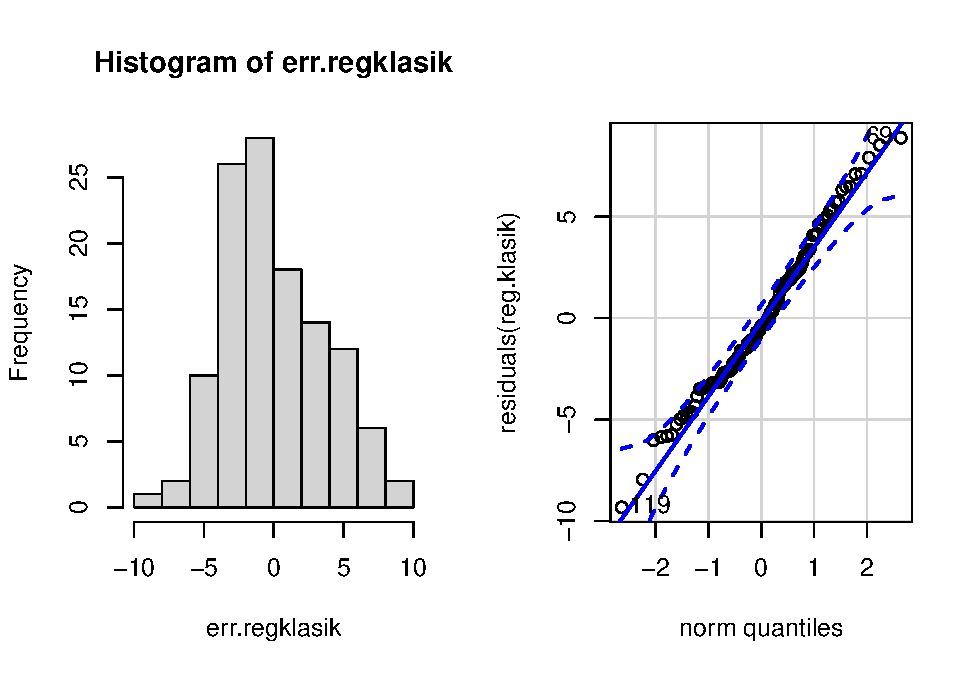
\includegraphics{modul_files/figure-latex/unnamed-chunk-56-1.pdf}

\begin{verbatim}
## [1] 119  69
\end{verbatim}

\begin{quote}
H0: galat model menyebar normal
\end{quote}

\begin{quote}
H1: galat model tidak menyebar normal
\end{quote}

\hypertarget{kehomogenan-ragam-sisaan}{%
\subsection{Kehomogenan Ragam Sisaan}\label{kehomogenan-ragam-sisaan}}

\begin{Shaded}
\begin{Highlighting}[]
\FunctionTok{plot}\NormalTok{(}\FunctionTok{fitted}\NormalTok{(reg.klasik), }\FunctionTok{residuals}\NormalTok{(reg.klasik))}
\end{Highlighting}
\end{Shaded}

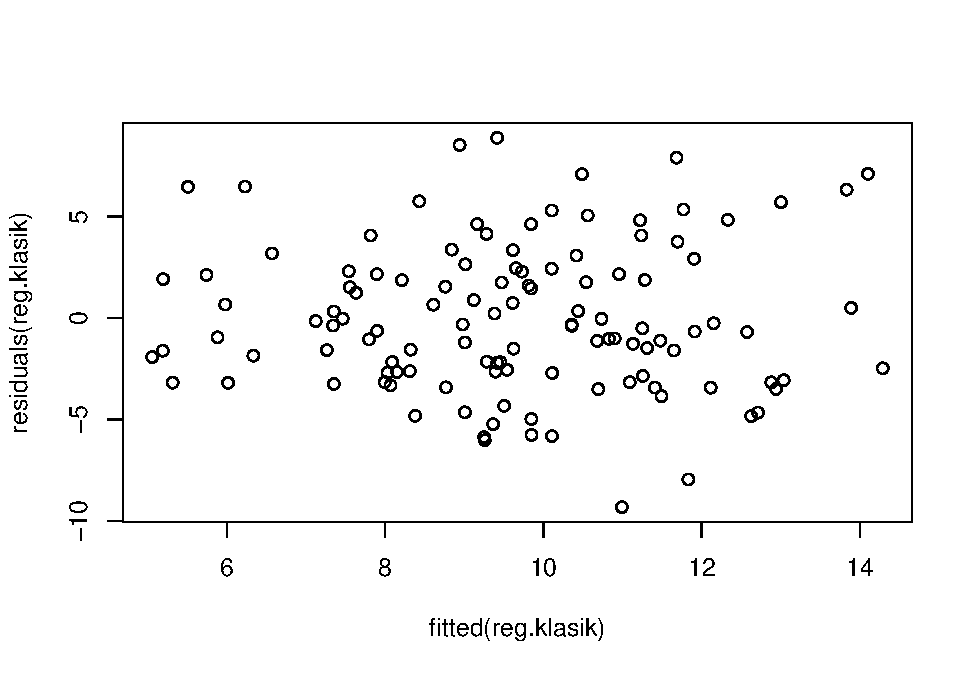
\includegraphics{modul_files/figure-latex/unnamed-chunk-57-1.pdf}

\begin{Shaded}
\begin{Highlighting}[]
\FunctionTok{bptest}\NormalTok{(reg.klasik)}
\end{Highlighting}
\end{Shaded}

\begin{verbatim}
## 
##  studentized Breusch-Pagan test
## 
## data:  reg.klasik
## BP = 3.979, df = 1, p-value = 0.04607
\end{verbatim}

\begin{quote}
H0: ragam galat homogen
\end{quote}

\begin{quote}
H1: ragam galat tidak homogen
\end{quote}

\hypertarget{kebebasan-sisaan}{%
\subsection{Kebebasan Sisaan}\label{kebebasan-sisaan}}

Uji kebebasan sisaan pada data spasial dapat dilakukan dengan uji moran menggunakan fungsi berikut.

\begin{Shaded}
\begin{Highlighting}[]
\NormalTok{w}\OtherTok{\textless{}{-}}\FunctionTok{poly2nb}\NormalTok{(petajawa)}
\NormalTok{ww}\OtherTok{\textless{}{-}}\FunctionTok{nb2listw}\NormalTok{(w, }\AttributeTok{zero.policy =}\NormalTok{T)}
\FunctionTok{lm.morantest}\NormalTok{(reg.klasik, ww, }\AttributeTok{alternative=}\StringTok{"two.sided"}\NormalTok{, }\AttributeTok{zero.policy =}\NormalTok{ T)}
\end{Highlighting}
\end{Shaded}

\begin{verbatim}
## 
##  Global Moran I for regression residuals
## 
## data:  
## model: lm(formula = Kemiskinan ~ Pendidikan, data = datajawa)
## weights: ww
## 
## Moran I statistic standard deviate = 5.3932, p-value = 6.922e-08
## alternative hypothesis: two.sided
## sample estimates:
## Observed Moran I      Expectation         Variance 
##      0.351747300     -0.011502703      0.004536512
\end{verbatim}

Selain menggunakan fungsi \texttt{lm.morantest}, uji moran dapat dilakukan menggunakan fungsi \texttt{moran.test} seperti yang dibahas pada modul pertemuan sebelumnya. Perbedaannya adalah pada fungsi pertama, input yang digunakan adalah objek \texttt{lm}, sedangkan pada fungsi kedua, yang digunakan sebagai input adalah data sisaan model.

\begin{Shaded}
\begin{Highlighting}[]
\FunctionTok{moran.test}\NormalTok{(err.regklasik, ww,}\AttributeTok{randomisation=}\NormalTok{F, }\AttributeTok{alternative=}\StringTok{"two.sided"}\NormalTok{, }\AttributeTok{zero.policy=}\NormalTok{T)}
\end{Highlighting}
\end{Shaded}

\begin{verbatim}
## 
##  Moran I test under normality
## 
## data:  err.regklasik  
## weights: ww  n reduced by no-neighbour observations
##   
## 
## Moran I statistic standard deviate = 5.3242, p-value = 1.014e-07
## alternative hypothesis: two.sided
## sample estimates:
## Moran I statistic       Expectation          Variance 
##       0.351747300      -0.008547009       0.004579345
\end{verbatim}

Terlihat pada output bahwa hasil kedua tes menunjukkan kesimpulan yang sama, yaitu tolak H0 yang menyatakan bahwa tidak terdapat autokorelasi pada sisaan model regresi klasik pada taraf nyata 5\%. Oleh karenanya, untuk mencari model yang lebih baik, kita dapat melakukan uji LM (lagrange multiplier) untuk mengidentifikasi model dependensi spasial yang dapat digunakan pada kasus ini.

\hypertarget{uji-lagrange-multiplier}{%
\section{Uji Lagrange Multiplier}\label{uji-lagrange-multiplier}}

\begin{Shaded}
\begin{Highlighting}[]
\NormalTok{LM}\OtherTok{\textless{}{-}}\FunctionTok{lm.LMtests}\NormalTok{(reg.klasik, }\FunctionTok{nb2listw}\NormalTok{(w, }\AttributeTok{style=}\StringTok{"W"}\NormalTok{, }\AttributeTok{zero.policy=}\NormalTok{T),}
               \AttributeTok{test=}\FunctionTok{c}\NormalTok{(}\StringTok{"LMerr"}\NormalTok{, }\StringTok{"LMlag"}\NormalTok{,}\StringTok{"RLMerr"}\NormalTok{,}\StringTok{"RLMlag"}\NormalTok{,}\StringTok{"SARMA"}\NormalTok{), }\AttributeTok{zero.policy=}\NormalTok{T)}
\FunctionTok{summary}\NormalTok{(LM)}
\end{Highlighting}
\end{Shaded}

\begin{verbatim}
##  Lagrange multiplier diagnostics for spatial dependence
## data:  
## model: lm(formula = Kemiskinan ~ Pendidikan, data = datajawa)
## weights: nb2listw(w, style = "W", zero.policy = T)
##  
##        statistic parameter   p.value    
## LMerr    26.4886         1 2.651e-07 ***
## LMlag    27.2100         1 1.825e-07 ***
## RLMerr    1.4217         1    0.2331    
## RLMlag    2.1431         1    0.1432    
## SARMA    28.6317         2 6.063e-07 ***
## ---
## Signif. codes:  0 '***' 0.001 '**' 0.01 '*' 0.05 '.' 0.1 ' ' 1
\end{verbatim}

Output memperlihatkan bahwa hasil uji model SEM dan SAR sama-sama signifikan pada taraf 5\%. Selanjutnya, hasil uji robust keduanya ternyata sama-sama tidak signifikan. Berdasarkan skema tersebut, kita dapat mencoba kandidat model SARMA atau GSM. Namun demikian, ada pula pendapat yang menyarankan agar kita mengambil kandidat model dengan p-value terkecil, pada kasus ini p-value terkecil juga terdapat pada model SARMA atau GSM.

Mohon diingat bahwa pada ilustrasi yang kita lakukan saat ini, kita hanya menggunakan satu peubah bebas sehingga kita tidak perlu mengkhawatirkan masalah multikolinieritas. Pada saat Anda memiliki lebih dari satu peubah bebas, pastikan Anda juga memperhatikan multikolinieritas pada model. Pemeriksaan dapat dilakukan dengan fungsi \texttt{vif()} pada package \texttt{car}.

\hypertarget{pemodelan-regresi-spasial}{%
\section{Pemodelan Regresi Spasial}\label{pemodelan-regresi-spasial}}

Pada modul ini, untuk kepentingan pembelajaran, kita akan mencoba ketiga model, SEM, SAR, dan SARMA, meskipun pada prakteknya, Anda hanya perlu memodelkan yang menurut Anda terbaik saja.

\begin{Shaded}
\begin{Highlighting}[]
\NormalTok{w}\OtherTok{\textless{}{-}}\FunctionTok{poly2nb}\NormalTok{(petajawa)}
\NormalTok{ww}\OtherTok{\textless{}{-}}\FunctionTok{nb2listw}\NormalTok{(w, }\AttributeTok{zero.policy=}\NormalTok{T)}
\end{Highlighting}
\end{Shaded}

\hypertarget{model-sem}{%
\subsection{Model SEM}\label{model-sem}}

\begin{Shaded}
\begin{Highlighting}[]
\FunctionTok{library}\NormalTok{(spatialreg)}

\NormalTok{sem}\OtherTok{\textless{}{-}}\FunctionTok{errorsarlm}\NormalTok{(Kemiskinan}\SpecialCharTok{\textasciitilde{}}\NormalTok{Pendidikan,}\AttributeTok{data=}\NormalTok{datajawa,ww, }\AttributeTok{zero.policy=}\NormalTok{T)}
\FunctionTok{summary}\NormalTok{(sem)}
\end{Highlighting}
\end{Shaded}

\begin{verbatim}
## 
## Call:errorsarlm(formula = Kemiskinan ~ Pendidikan, data = datajawa, 
##     listw = ww, zero.policy = T)
## 
## Residuals:
##      Min       1Q   Median       3Q      Max 
## -7.04950 -1.86484 -0.43797  1.87675  8.14992 
## 
## Type: error 
## Regions with no neighbours included:
##  0 
## Coefficients: (asymptotic standard errors) 
##             Estimate Std. Error z value  Pr(>|z|)
## (Intercept) 6.359121   0.958495  6.6345 3.256e-11
## Pendidikan  0.114932   0.029332  3.9183 8.918e-05
## 
## Lambda: 0.57487, LR test value: 29.606, p-value: 5.2937e-08
## Asymptotic standard error: 0.083992
##     z-value: 6.8443, p-value: 7.6856e-12
## Wald statistic: 46.844, p-value: 7.6857e-12
## 
## Log likelihood: -307.7876 for error model
## ML residual variance (sigma squared): 9.4425, (sigma: 3.0729)
## Number of observations: 119 
## Number of parameters estimated: 4 
## AIC: 623.58, (AIC for lm: 651.18)
\end{verbatim}

\begin{Shaded}
\begin{Highlighting}[]
\NormalTok{pseudoR2.sem}\OtherTok{\textless{}{-}}\FunctionTok{cor}\NormalTok{(datajawa}\SpecialCharTok{$}\NormalTok{Kemiskinan, }\FunctionTok{fitted}\NormalTok{(sem))}\SpecialCharTok{\^{}}\DecValTok{2}
\NormalTok{pseudoR2.sem}
\end{Highlighting}
\end{Shaded}

\begin{verbatim}
## [1] 0.4786585
\end{verbatim}

Output di atas menunjukkan bahwa koefisien Lambda signifikan pada taraf nyata 5\% ( p-value = 5.2937e-08 ). AIC model SEM adalah sebesar 623.58, dengan pseudo-\(R^2=0.4787\) Selanjutnya kita akan coba memeriksa sisaan model SEM ini.

\begin{Shaded}
\begin{Highlighting}[]
\FunctionTok{library}\NormalTok{(nortest)}
\NormalTok{err.sem}\OtherTok{\textless{}{-}}\FunctionTok{residuals}\NormalTok{(sem)}
\FunctionTok{shapiro.test}\NormalTok{(err.sem)}
\end{Highlighting}
\end{Shaded}

\begin{verbatim}
## 
##  Shapiro-Wilk normality test
## 
## data:  err.sem
## W = 0.98234, p-value = 0.1208
\end{verbatim}

\begin{Shaded}
\begin{Highlighting}[]
\FunctionTok{bptest.sarlm}\NormalTok{(sem)}
\end{Highlighting}
\end{Shaded}

\begin{verbatim}
## 
##  studentized Breusch-Pagan test
## 
## data:  
## BP = 4.1883, df = 1, p-value = 0.0407
\end{verbatim}

\begin{Shaded}
\begin{Highlighting}[]
\FunctionTok{moran.test}\NormalTok{(err.sem, ww, }\AttributeTok{alternative=}\StringTok{"two.sided"}\NormalTok{, }\AttributeTok{zero.policy=}\NormalTok{T)}
\end{Highlighting}
\end{Shaded}

\begin{verbatim}
## 
##  Moran I test under randomisation
## 
## data:  err.sem  
## weights: ww  n reduced by no-neighbour observations
##   
## 
## Moran I statistic standard deviate = -0.53535, p-value = 0.5924
## alternative hypothesis: two.sided
## sample estimates:
## Moran I statistic       Expectation          Variance 
##      -0.044773446      -0.008547009       0.004579087
\end{verbatim}

Terlihat pada output di atas bahwa sisaan memenuhi asumsi kenormalan dan asumsi kebebasan.

\hypertarget{model-sar}{%
\subsection{Model SAR}\label{model-sar}}

\begin{Shaded}
\begin{Highlighting}[]
\NormalTok{sar}\OtherTok{\textless{}{-}}\FunctionTok{lagsarlm}\NormalTok{(Kemiskinan}\SpecialCharTok{\textasciitilde{}}\NormalTok{Pendidikan,}\AttributeTok{data=}\NormalTok{datajawa,ww, }\AttributeTok{zero.policy=}\NormalTok{T)}
\FunctionTok{summary}\NormalTok{(sar)}
\end{Highlighting}
\end{Shaded}

\begin{verbatim}
## 
## Call:lagsarlm(formula = Kemiskinan ~ Pendidikan, data = datajawa, 
##     listw = ww, zero.policy = T)
## 
## Residuals:
##      Min       1Q   Median       3Q      Max 
## -7.17361 -1.97250 -0.56646  1.82449  9.57815 
## 
## Type: lag 
## Regions with no neighbours included:
##  0 
## Coefficients: (asymptotic standard errors) 
##             Estimate Std. Error z value  Pr(>|z|)
## (Intercept) 1.779095   0.992235  1.7930   0.07297
## Pendidikan  0.117724   0.027717  4.2473 2.164e-05
## 
## Rho: 0.46783, LR test value: 25.624, p-value: 4.1491e-07
## Asymptotic standard error: 0.087013
##     z-value: 5.3766, p-value: 7.5901e-08
## Wald statistic: 28.908, p-value: 7.5901e-08
## 
## Log likelihood: -309.7788 for lag model
## ML residual variance (sigma squared): 10.098, (sigma: 3.1777)
## Number of observations: 119 
## Number of parameters estimated: 4 
## AIC: 627.56, (AIC for lm: 651.18)
## LM test for residual autocorrelation
## test value: 0.014268, p-value: 0.90492
\end{verbatim}

\begin{Shaded}
\begin{Highlighting}[]
\NormalTok{pseudoR2.sar}\OtherTok{\textless{}{-}}\FunctionTok{cor}\NormalTok{(datajawa}\SpecialCharTok{$}\NormalTok{Kemiskinan, }\FunctionTok{fitted}\NormalTok{(sar))}\SpecialCharTok{\^{}}\DecValTok{2}
\NormalTok{pseudoR2.sar}
\end{Highlighting}
\end{Shaded}

\begin{verbatim}
## [1] 0.4292466
\end{verbatim}

Output di atas memperlihatkan bahwa koefisien Rho pada model SAR signifikan, dengan nilai AIC sebesar 627.56 dengan pseudo-\(R^2=0.4292\) . Selain itu, terlihat pula hasil uji autokorelasi pada sisaan model memperlihatkan nilai p-value sebesar 0.90492, artinya tidak terdapat autokorelasi pada sisaan.

\begin{Shaded}
\begin{Highlighting}[]
\NormalTok{err.sar}\OtherTok{\textless{}{-}}\FunctionTok{residuals}\NormalTok{(sar)}
\FunctionTok{shapiro.test}\NormalTok{(err.sar)}
\end{Highlighting}
\end{Shaded}

\begin{verbatim}
## 
##  Shapiro-Wilk normality test
## 
## data:  err.sar
## W = 0.98005, p-value = 0.07421
\end{verbatim}

\begin{Shaded}
\begin{Highlighting}[]
\FunctionTok{bptest.sarlm}\NormalTok{(sar)}
\end{Highlighting}
\end{Shaded}

\begin{verbatim}
## 
##  studentized Breusch-Pagan test
## 
## data:  
## BP = 1.6725, df = 1, p-value = 0.1959
\end{verbatim}

\begin{Shaded}
\begin{Highlighting}[]
\FunctionTok{moran.test}\NormalTok{(err.sar, ww, }\AttributeTok{alternative=}\StringTok{"two.sided"}\NormalTok{, }\AttributeTok{zero.policy=}\NormalTok{T)}
\end{Highlighting}
\end{Shaded}

\begin{verbatim}
## 
##  Moran I test under randomisation
## 
## data:  err.sar  
## weights: ww  n reduced by no-neighbour observations
##   
## 
## Moran I statistic standard deviate = 0.18303, p-value = 0.8548
## alternative hypothesis: two.sided
## sample estimates:
## Moran I statistic       Expectation          Variance 
##       0.003823646      -0.008547009       0.004567919
\end{verbatim}

Berdasarkan output di atas, pada taraf 5\% dapat disimpulkan bahwa sisaan model memenuhi asumsi kenormalan, kehomogenan ragam, dan kebebasan.

\hypertarget{model-gsmsarma}{%
\subsection{Model GSM/SARMA}\label{model-gsmsarma}}

\begin{Shaded}
\begin{Highlighting}[]
\NormalTok{gsm}\OtherTok{\textless{}{-}}\FunctionTok{sacsarlm}\NormalTok{(Kemiskinan}\SpecialCharTok{\textasciitilde{}}\NormalTok{Pendidikan,}\AttributeTok{data=}\NormalTok{datajawa,ww, }\AttributeTok{zero.policy=}\NormalTok{T)}
\FunctionTok{summary}\NormalTok{(gsm)}
\end{Highlighting}
\end{Shaded}

\begin{verbatim}
## 
## Call:sacsarlm(formula = Kemiskinan ~ Pendidikan, data = datajawa, 
##     listw = ww, zero.policy = T)
## 
## Residuals:
##      Min       1Q   Median       3Q      Max 
## -6.20932 -1.69855 -0.38001  1.70634  7.26252 
## 
## Type: sac 
## Coefficients: (asymptotic standard errors) 
##              Estimate Std. Error z value Pr(>|z|)
## (Intercept) 10.338070   1.750226  5.9067 3.49e-09
## Pendidikan   0.099813   0.027137  3.6781 0.000235
## 
## Rho: -0.43058
## Asymptotic standard error: 0.14723
##     z-value: -2.9246, p-value: 0.0034494
## Lambda: 0.79882
## Asymptotic standard error: 0.069513
##     z-value: 11.492, p-value: < 2.22e-16
## 
## LR test value: 34.317, p-value: 3.5325e-08
## 
## Log likelihood: -305.432 for sac model
## ML residual variance (sigma squared): 7.7401, (sigma: 2.7821)
## Number of observations: 119 
## Number of parameters estimated: 5 
## AIC: 620.86, (AIC for lm: 651.18)
\end{verbatim}

\begin{Shaded}
\begin{Highlighting}[]
\NormalTok{pseudoR2.gsm}\OtherTok{\textless{}{-}}\FunctionTok{cor}\NormalTok{(datajawa}\SpecialCharTok{$}\NormalTok{Kemiskinan, }\FunctionTok{fitted}\NormalTok{(gsm))}\SpecialCharTok{\^{}}\DecValTok{2}
\NormalTok{pseudoR2.gsm}
\end{Highlighting}
\end{Shaded}

\begin{verbatim}
## [1] 0.5933811
\end{verbatim}

Output di atas memperlihatkan bahwa kedua koefisien dependensi spasial, Rho dan Lambda signifikan. AIC model SARMA adalah sebesar 620.86 dengan pseudo-\(R^2=0.5934\)

\begin{Shaded}
\begin{Highlighting}[]
\NormalTok{err.gsm}\OtherTok{\textless{}{-}}\FunctionTok{residuals}\NormalTok{(gsm)}
\FunctionTok{shapiro.test}\NormalTok{(err.gsm)}
\end{Highlighting}
\end{Shaded}

\begin{verbatim}
## 
##  Shapiro-Wilk normality test
## 
## data:  err.gsm
## W = 0.98527, p-value = 0.2219
\end{verbatim}

\begin{Shaded}
\begin{Highlighting}[]
\FunctionTok{bptest.sarlm}\NormalTok{(gsm)}
\end{Highlighting}
\end{Shaded}

\begin{verbatim}
## 
##  studentized Breusch-Pagan test
## 
## data:  
## BP = 2.3236, df = 1, p-value = 0.1274
\end{verbatim}

\begin{Shaded}
\begin{Highlighting}[]
\FunctionTok{moran.test}\NormalTok{(err.gsm, ww, }\AttributeTok{alternative=}\StringTok{"two.sided"}\NormalTok{, }\AttributeTok{zero.policy=}\NormalTok{T)}
\end{Highlighting}
\end{Shaded}

\begin{verbatim}
## 
##  Moran I test under randomisation
## 
## data:  err.gsm  
## weights: ww  n reduced by no-neighbour observations
##   
## 
## Moran I statistic standard deviate = -0.17988, p-value = 0.8572
## alternative hypothesis: two.sided
## sample estimates:
## Moran I statistic       Expectation          Variance 
##      -0.020720135      -0.008547009       0.004579838
\end{verbatim}

Berdasarkan output di atas, terlihat bahwa sisaan model SARMA telah memenuhi asumsi kenormalan, kehomogenan ragam, dan kebebasan.

\hypertarget{penentuan-model-terbaik}{%
\subsection{Penentuan Model Terbaik}\label{penentuan-model-terbaik}}

Akhirnya, kita akan coba merangkum hasil pemodelan yang telah dilakukan sepanjang ilustrasi pada modul ini.

\captionsetup[table]{labelformat=empty,skip=1pt}
\begin{longtable}{lrrrr}
\toprule
Rincian & OLS & SEM & SAR & SARMA \\ 
\midrule
AIC & 651.180 & 623.580 & 627.560 & 620.860 \\ 
pseudo-R2 & 0.246 & 0.479 & 0.429 & 0.593 \\ 
p-value of Rho & NA & NA & 0.000 & 0.000 \\ 
p-value of Lambda & NA & 0.000 & NA & 0.003 \\ 
Kenormalan(p-value) & 0.261 & 0.121 & 0.074 & 0.222 \\ 
Homoskedastisitas (p-value) & 0.046 & 0.041 & 0.196 & 0.127 \\ 
Kebebasan Sisaan(p-value) & 0.000 & 0.592 & 0.855 & 0.857 \\ 
\bottomrule
\end{longtable}

Ilustrasi pada kasus ini memperlihatkan bahwa ternyata GSM merupakan model terbaik berdasarkan nilai AIC dan pseudo-\(R^2\). Hal ini ternyata konsisten dengan p-value nya yang juga terkecil pada uji-LM.

\hypertarget{efek-marginal}{%
\section{Efek Marginal}\label{efek-marginal}}

Efek marginal atau limpahan (\emph{spill-over}) adalah besarnya dampak perubahan pada peubah dependen pada wilayah-\(i\), akibat perubahan prediktor di wilayah-\(j\).

Efek marginal terdapat pada model dependensi spasial SAR, GSM, SDM, SDEM, dan SLX. Efek ini dapat dibedakan menjadi tiga, yaitu efek langsung (\emph{direct effect}), efek tidak langsung (\emph{indirect effect}), dan efek total (\emph{total effect}).

\begin{Shaded}
\begin{Highlighting}[]
\FunctionTok{impacts}\NormalTok{(gsm, }\AttributeTok{listw=}\NormalTok{ww)}
\end{Highlighting}
\end{Shaded}

\begin{verbatim}
## Impact measures (sac, exact):
##               Direct    Indirect      Total
## Pendidikan 0.1038916 -0.03386839 0.07002321
\end{verbatim}

Output di atas menunjukkan bahwa pertambahan satu satuan pada pendidikan di suatu wilayah akan diikuti oleh peningkatan kemiskinan di wilayah tersebut sebesar rata-rata 0.1938916 (pengaruh langsung), sedangkan pada wilayah tetangganya akan mengalami penurunan kemiskinan rata-rata sebesar 0.03386839 (pengaruh tak langsung).

\hypertarget{latihan}{%
\section{Latihan}\label{latihan}}

Sebagai latihan, silahkan lakukan pemodelan menggunakan data \texttt{Kemiskinan} di Pulau Jawa dengan peubah bebas ruta penerima raskin dan persentase pendidikan yang ditamatkan di bawah SD.

\begin{itemize}
\item
  periksa multikolineritas antar peubah bebas yang digunakan berdasarkan VIF
\item
  eksplorasi autokorelasi spasial pada model menggunakan jarak \texttt{W\_dist}
\item
  lakukan pemodelan yang menurut Anda paling tepat, interpretasikan.
\end{itemize}

\hypertarget{sumber-pustaka-1}{%
\section{Sumber Pustaka}\label{sumber-pustaka-1}}

Guliyev, H. (2020). Determining the spatial effects of COVID-19 using the spatial panel data model. Spatial Statistics, 100443. \url{doi:10.1016/j.spasta.2020.100443}. Retrieved from: \url{https://www.ncbi.nlm.nih.gov/pmc/articles/PMC7139267/}

Sarmiento-Barbieri, I. (2016, April 24). An introduction to spatial econometrics in R. Spatial Econometric Workshop, University of Illinois. Retrieved from: \url{https://www.econ.uiuc.edu/~lab/workshop/Spatial_in_R.html\#modeling-spatial-dependence}

Zhukov, Y. M. (2010, January 19). Applied Spatial Statistics in R, Section 6, Spatial Regression {[}PDF slides.{]}. IQSS, Harvard University. Retrieved from: \url{http://www.people.fas.harvard.edu/~zhukov/Spatial6.pdf}

\hypertarget{geographically-weighted-regression-gwr}{%
\chapter{Geographically Weighted Regression (GWR)}\label{geographically-weighted-regression-gwr}}

Suatu pemodelan dapat bersifat global maupun lokal. Regresi linier klasik merupakan salah satu model global. Dikatakan global karena terdapat satu model yang berlaku umum untuk semua pengamatan.

Suatu model lokal bersifat lebih fleksibel, yang dalam konteks spasial, artinya setiap daerah/lokasi dapat memiliki model masing-masing.

Geographically Weighted Regression (GWR) merupakan salah satu model yang bersifat lokal. Beberapa keuntungan dengen menggunakan model ini, diantaranya adalah kita dapat:

\begin{itemize}
\item
  menduga galat baku lokal
\item
  menghitung ukuran leverage lokal
\item
  melakukan pengujian terhadap signifikansi keragaman spasial pada penduga parameter lokal
\item
  menguji apakah model lokal lebih baik daripada model global
\end{itemize}

Terdapat salah satu \emph{stand-alone software} untuk melakukan GWR, yaitu software GWR yang dapat diakses melalui \url{http://ncg.nuim.ie/ncg/GWR/}. Selain itu, pada R software, terdapat beberapa package yang dapat digunakan untuk membangun model GWR, yaitu:

\begin{itemize}
\item
  GWmodel
\item
  spgwr
\item
  gwrr
\end{itemize}

Pada modul ini akan dibahas pemodelan GWR menggunakan package \texttt{spgwr}.

\hypertarget{eksplorasi-data-1}{%
\section{Eksplorasi Data}\label{eksplorasi-data-1}}

\begin{Shaded}
\begin{Highlighting}[]
\FunctionTok{library}\NormalTok{(rgdal)}
\NormalTok{petajawa}\OtherTok{=}\FunctionTok{readOGR}\NormalTok{(}\AttributeTok{dsn=}\StringTok{"Jawamap"}\NormalTok{, }\AttributeTok{layer=}\StringTok{"jawa"}\NormalTok{)}
\end{Highlighting}
\end{Shaded}

\begin{verbatim}
## OGR data source with driver: ESRI Shapefile 
## Source: "D:\Jobs\Pelatihan Spasial STIS\New folder\Pelatihan-Spasial\Jawamap", layer: "jawa"
## with 119 features
## It has 5 fields
\end{verbatim}

\begin{Shaded}
\begin{Highlighting}[]
\NormalTok{datajawa}\OtherTok{=}\FunctionTok{read.csv}\NormalTok{(}\StringTok{"Pulau Jawa.csv"}\NormalTok{, }\AttributeTok{header=}\NormalTok{T, }\AttributeTok{sep=}\StringTok{";"}\NormalTok{)}
\NormalTok{petajawa}\SpecialCharTok{$}\NormalTok{Kemiskinan}\OtherTok{\textless{}{-}}\NormalTok{ datajawa}\SpecialCharTok{$}\NormalTok{Kemiskinan}
\end{Highlighting}
\end{Shaded}

Plot berikut ini dapat dimanfaatkan untuk mengeksplorasi hubungan antar peubah.

\begin{Shaded}
\begin{Highlighting}[]
\NormalTok{corr}\OtherTok{\textless{}{-}}\FunctionTok{cor}\NormalTok{(datajawa[,}\SpecialCharTok{{-}}\NormalTok{(}\DecValTok{1}\SpecialCharTok{:}\DecValTok{4}\NormalTok{)])}
\NormalTok{corrplot}\SpecialCharTok{::}\FunctionTok{corrplot}\NormalTok{(corr, }\AttributeTok{is.corr=}\NormalTok{T)}
\end{Highlighting}
\end{Shaded}

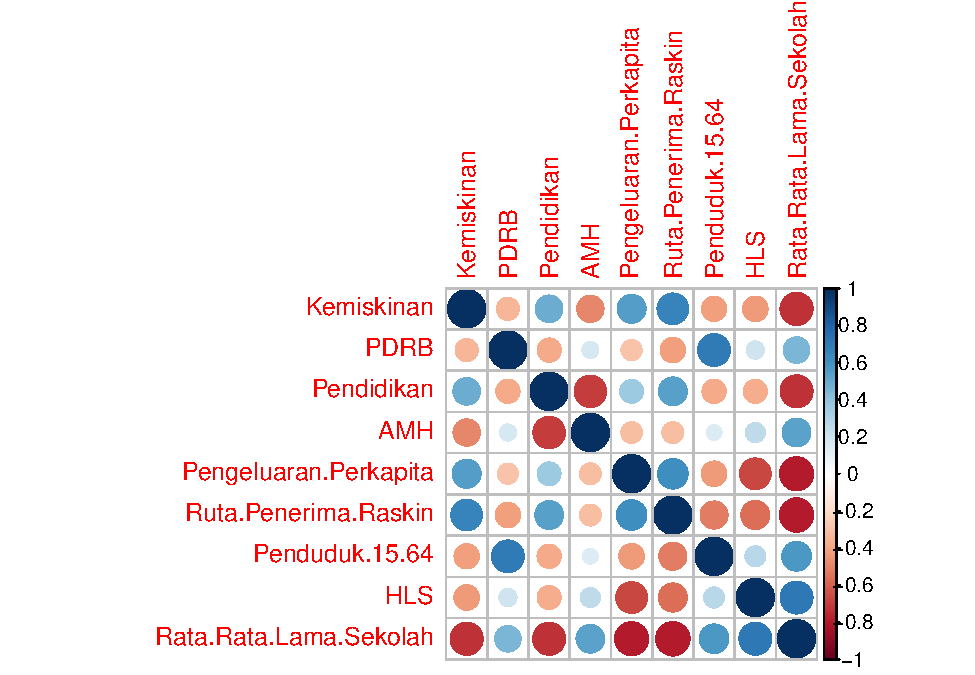
\includegraphics{modul_files/figure-latex/unnamed-chunk-71-1.pdf}

Sebagai ilustrasi, peubah rata-rata lama sekolah akan digunakan untuk memodelkan kemiskinan di pulau Jawa. Sebagai langkah awal, kita akan terlebih dulu memodelkannya menggunakan regresi linear.

\begin{Shaded}
\begin{Highlighting}[]
\NormalTok{fit.lm}\OtherTok{\textless{}{-}}\FunctionTok{lm}\NormalTok{(Kemiskinan}\SpecialCharTok{\textasciitilde{}}\NormalTok{Rata.Rata.Lama.Sekolah, }\AttributeTok{data=}\NormalTok{datajawa)}
\FunctionTok{summary}\NormalTok{(fit.lm)}
\end{Highlighting}
\end{Shaded}

\begin{verbatim}
## 
## Call:
## lm(formula = Kemiskinan ~ Rata.Rata.Lama.Sekolah, data = datajawa)
## 
## Residuals:
##     Min      1Q  Median      3Q     Max 
## -7.0384 -1.9865 -0.3389  1.6722  9.7042 
## 
## Coefficients:
##                        Estimate Std. Error t value Pr(>|t|)    
## (Intercept)             24.7340     1.3417   18.44   <2e-16 ***
## Rata.Rata.Lama.Sekolah  -1.8657     0.1624  -11.49   <2e-16 ***
## ---
## Signif. codes:  0 '***' 0.001 '**' 0.01 '*' 0.05 '.' 0.1 ' ' 1
## 
## Residual standard error: 2.898 on 117 degrees of freedom
## Multiple R-squared:  0.5302, Adjusted R-squared:  0.5262 
## F-statistic:   132 on 1 and 117 DF,  p-value: < 2.2e-16
\end{verbatim}

Selanjutnya, diagnostik model dilakukan untuk memeriksa pemenuhan asumsi pada model regresi linear.

\begin{Shaded}
\begin{Highlighting}[]
\NormalTok{err.lm}\OtherTok{\textless{}{-}}\FunctionTok{residuals}\NormalTok{(fit.lm)}
\FunctionTok{shapiro.test}\NormalTok{(err.lm)}
\end{Highlighting}
\end{Shaded}

\begin{verbatim}
## 
##  Shapiro-Wilk normality test
## 
## data:  err.lm
## W = 0.98029, p-value = 0.07818
\end{verbatim}

\begin{Shaded}
\begin{Highlighting}[]
\FunctionTok{par}\NormalTok{(}\AttributeTok{mfrow=}\FunctionTok{c}\NormalTok{(}\DecValTok{1}\NormalTok{,}\DecValTok{2}\NormalTok{))}
\FunctionTok{hist}\NormalTok{(err.lm)}
\NormalTok{car}\SpecialCharTok{::}\FunctionTok{qqPlot}\NormalTok{(}\FunctionTok{residuals}\NormalTok{(fit.lm))}
\end{Highlighting}
\end{Shaded}

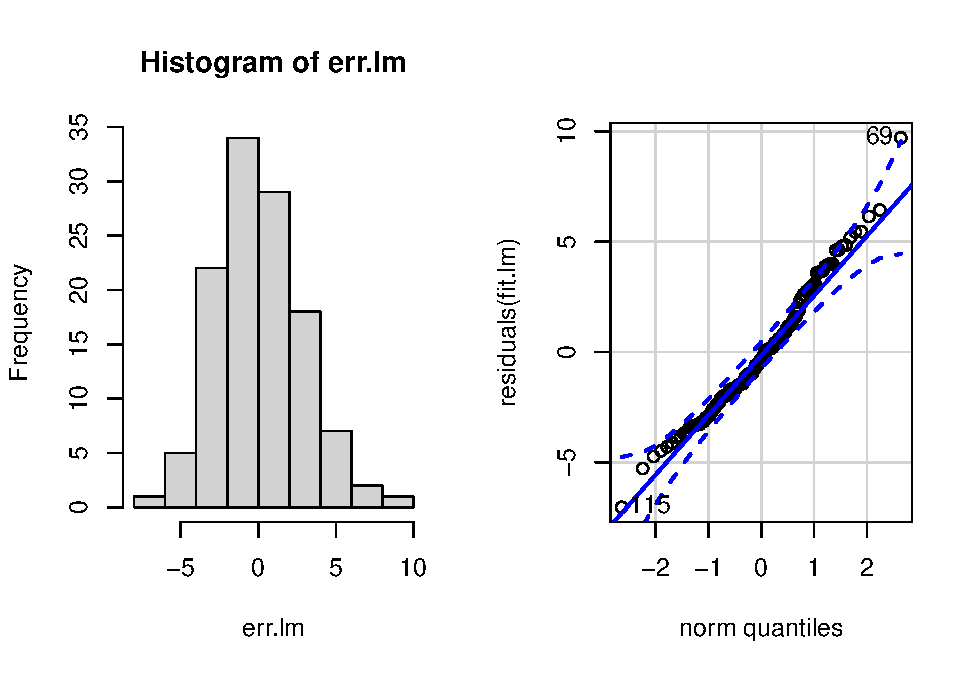
\includegraphics{modul_files/figure-latex/unnamed-chunk-73-1.pdf}

\begin{verbatim}
## [1]  69 115
\end{verbatim}

\begin{Shaded}
\begin{Highlighting}[]
\FunctionTok{plot}\NormalTok{(fit.lm,}\AttributeTok{which=}\DecValTok{1}\NormalTok{)}
\NormalTok{lmtest}\SpecialCharTok{::}\FunctionTok{bptest}\NormalTok{(fit.lm)}
\end{Highlighting}
\end{Shaded}

\begin{verbatim}
## 
##  studentized Breusch-Pagan test
## 
## data:  fit.lm
## BP = 4.7982, df = 1, p-value = 0.02849
\end{verbatim}

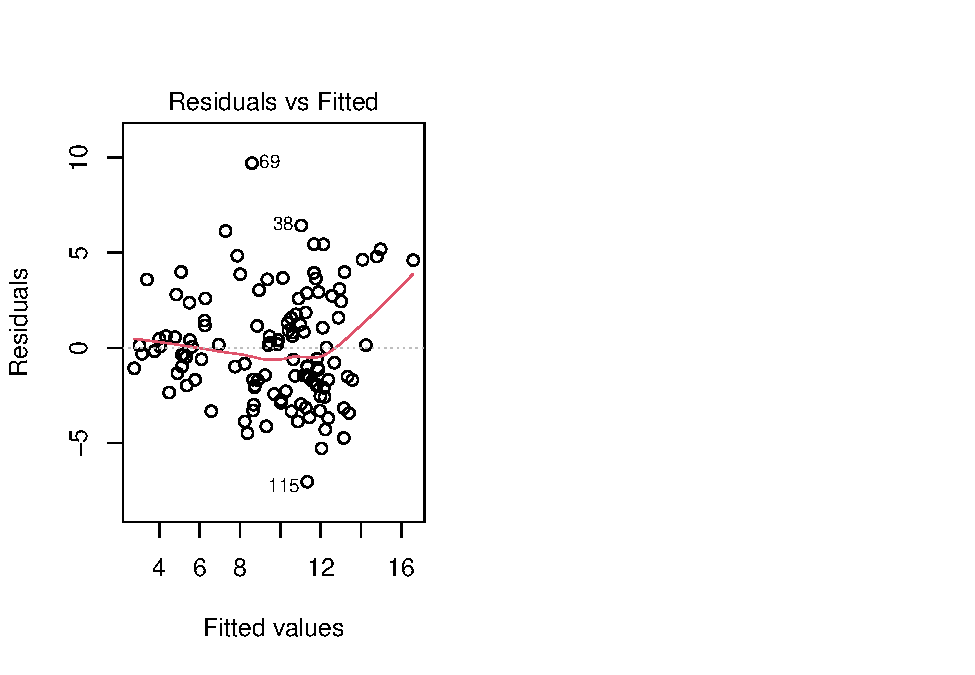
\includegraphics{modul_files/figure-latex/unnamed-chunk-73-2.pdf}

Terlihat pada output di atas bahwa sisaan model cenderung memiliki ragam yang tidak konstan. Selanjutnya juga akan diperiksa kebebasan sisaan menggunakan uji moran.

\begin{Shaded}
\begin{Highlighting}[]
\FunctionTok{library}\NormalTok{(spdep)}
\NormalTok{w}\OtherTok{\textless{}{-}}\FunctionTok{poly2nb}\NormalTok{(petajawa)}
\NormalTok{ww}\OtherTok{\textless{}{-}}\FunctionTok{nb2listw}\NormalTok{(w, }\AttributeTok{zero.policy=}\NormalTok{T)}

\FunctionTok{lm.morantest}\NormalTok{(fit.lm, ww, }\AttributeTok{alternative=}\StringTok{"two.sided"}\NormalTok{, }\AttributeTok{zero.policy =}\NormalTok{ T)}
\end{Highlighting}
\end{Shaded}

\begin{verbatim}
## 
##  Global Moran I for regression residuals
## 
## data:  
## model: lm(formula = Kemiskinan ~ Rata.Rata.Lama.Sekolah, data =
## datajawa)
## weights: ww
## 
## Moran I statistic standard deviate = 5.9602, p-value = 2.519e-09
## alternative hypothesis: two.sided
## sample estimates:
## Observed Moran I      Expectation         Variance 
##       0.38842759      -0.01284003       0.00453256
\end{verbatim}

Terlihat pada output bahwa terdapat autokorelasi spasial pada sisaan model regresi linier. Dengan mempertimbangkan bahwa sisaan model memiliki ragam yang tidak homogen, serta memiliki autokorelasi spasial, kita selanjutnya dapat mencoba memodelkannya dengan model regresi terboboti geografis atau GWR. Namun pada modul pembelajaran ini, kami akan perlihatkan pula bahwa pada pemodelan regresi spasial pun ternyata tetap menghasilkan sisaan dengan ragam yang heterogen.

\begin{Shaded}
\begin{Highlighting}[]
\NormalTok{LM}\OtherTok{\textless{}{-}}\FunctionTok{lm.LMtests}\NormalTok{(fit.lm, ww,}\AttributeTok{test=}\FunctionTok{c}\NormalTok{(}\StringTok{"LMerr"}\NormalTok{, }\StringTok{"LMlag"}\NormalTok{,}\StringTok{"RLMerr"}\NormalTok{,}\StringTok{"RLMlag"}\NormalTok{,}\StringTok{"SARMA"}\NormalTok{), }\AttributeTok{zero.policy=}\NormalTok{T)}
\FunctionTok{summary}\NormalTok{(LM)}
\end{Highlighting}
\end{Shaded}

\begin{verbatim}
##  Lagrange multiplier diagnostics for spatial dependence
## data:  
## model: lm(formula = Kemiskinan ~ Rata.Rata.Lama.Sekolah, data =
## datajawa)
## weights: ww
##  
##         statistic parameter   p.value    
## LMerr  32.3011683         1 1.320e-08 ***
## LMlag  18.2380122         1 1.949e-05 ***
## RLMerr 14.0653693         1 0.0001766 ***
## RLMlag  0.0022132         1 0.9624773    
## SARMA  32.3033815         2 9.670e-08 ***
## ---
## Signif. codes:  0 '***' 0.001 '**' 0.01 '*' 0.05 '.' 0.1 ' ' 1
\end{verbatim}

\begin{Shaded}
\begin{Highlighting}[]
\FunctionTok{library}\NormalTok{(spatialreg)}
\NormalTok{sem}\OtherTok{\textless{}{-}}\FunctionTok{errorsarlm}\NormalTok{(Kemiskinan}\SpecialCharTok{\textasciitilde{}}\NormalTok{Rata.Rata.Lama.Sekolah,}\AttributeTok{data=}\NormalTok{datajawa,ww, }\AttributeTok{zero.policy=}\NormalTok{T)}
\NormalTok{sar}\OtherTok{\textless{}{-}}\FunctionTok{lagsarlm}\NormalTok{(Kemiskinan}\SpecialCharTok{\textasciitilde{}}\NormalTok{Rata.Rata.Lama.Sekolah,}\AttributeTok{data=}\NormalTok{datajawa,ww, }\AttributeTok{zero.policy=}\NormalTok{T)}
\NormalTok{gsm}\OtherTok{\textless{}{-}}\FunctionTok{sacsarlm}\NormalTok{(Kemiskinan}\SpecialCharTok{\textasciitilde{}}\NormalTok{Rata.Rata.Lama.Sekolah,}\AttributeTok{data=}\NormalTok{datajawa,ww, }\AttributeTok{zero.policy=}\NormalTok{T)}

\FunctionTok{bptest.sarlm}\NormalTok{(sem)}
\end{Highlighting}
\end{Shaded}

\begin{verbatim}
## 
##  studentized Breusch-Pagan test
## 
## data:  
## BP = 5.6364, df = 1, p-value = 0.01759
\end{verbatim}

\begin{Shaded}
\begin{Highlighting}[]
\FunctionTok{bptest.sarlm}\NormalTok{(sar)}
\end{Highlighting}
\end{Shaded}

\begin{verbatim}
## 
##  studentized Breusch-Pagan test
## 
## data:  
## BP = 4.0536, df = 1, p-value = 0.04408
\end{verbatim}

\begin{Shaded}
\begin{Highlighting}[]
\FunctionTok{bptest.sarlm}\NormalTok{(gsm)}
\end{Highlighting}
\end{Shaded}

\begin{verbatim}
## 
##  studentized Breusch-Pagan test
## 
## data:  
## BP = 3.8557, df = 1, p-value = 0.04958
\end{verbatim}

\hypertarget{basic-gwr}{%
\section{Basic GWR}\label{basic-gwr}}

Kita dapat menggunakan fungsi \texttt{gwr} pada package \texttt{spgwr} untuk menyusun model GWR pada R software, seperti pada program berikut ini.

\begin{Shaded}
\begin{Highlighting}[]
\FunctionTok{library}\NormalTok{(spgwr)}
\end{Highlighting}
\end{Shaded}

\begin{verbatim}
## Warning: package 'spgwr' was built under R version 4.0.4
\end{verbatim}

\begin{verbatim}
## NOTE: This package does not constitute approval of GWR
## as a method of spatial analysis; see example(gwr)
\end{verbatim}

\begin{Shaded}
\begin{Highlighting}[]
\FunctionTok{coordinates}\NormalTok{(datajawa)}\OtherTok{\textless{}{-}}\FunctionTok{c}\NormalTok{(}\StringTok{"Longitude"}\NormalTok{,}\StringTok{"Latitude"}\NormalTok{)}
\NormalTok{gwr20 }\OtherTok{\textless{}{-}} \FunctionTok{gwr}\NormalTok{(Kemiskinan}\SpecialCharTok{\textasciitilde{}}\NormalTok{Rata.Rata.Lama.Sekolah,}\AttributeTok{data=}\NormalTok{datajawa,}\AttributeTok{bandwidth=}\DecValTok{20}\NormalTok{)}
\NormalTok{gwr20}
\end{Highlighting}
\end{Shaded}

\begin{verbatim}
## Call:
## gwr(formula = Kemiskinan ~ Rata.Rata.Lama.Sekolah, data = datajawa, 
##     bandwidth = 20)
## Kernel function: gwr.Gauss 
## Fixed bandwidth: 20 
## Summary of GWR coefficient estimates at data points:
##                           Min. 1st Qu.  Median 3rd Qu.    Max.  Global
## X.Intercept.           24.6607 24.6971 24.7366 24.7620 24.8026 24.7340
## Rata.Rata.Lama.Sekolah -1.8708 -1.8673 -1.8651 -1.8617 -1.8585 -1.8657
\end{verbatim}

Kita dapat pula mengganti bandwidth sesuai dengan yang diinginkan. Selanjutnya kita akan bandingkan perbedaan akibat penentuan bandwidth yang berbeda-beda tersebut.

\begin{Shaded}
\begin{Highlighting}[]
\NormalTok{gwr3 }\OtherTok{\textless{}{-}} \FunctionTok{gwr}\NormalTok{(Kemiskinan}\SpecialCharTok{\textasciitilde{}}\NormalTok{Rata.Rata.Lama.Sekolah,}\AttributeTok{data=}\NormalTok{datajawa, }\AttributeTok{bandwidth=}\DecValTok{3}\NormalTok{)}
\NormalTok{gwr3}
\end{Highlighting}
\end{Shaded}

\begin{verbatim}
## Call:
## gwr(formula = Kemiskinan ~ Rata.Rata.Lama.Sekolah, data = datajawa, 
##     bandwidth = 3)
## Kernel function: gwr.Gauss 
## Fixed bandwidth: 3 
## Summary of GWR coefficient estimates at data points:
##                           Min. 1st Qu.  Median 3rd Qu.    Max.  Global
## X.Intercept.           21.8567 23.3823 24.6838 25.4191 26.4774 24.7340
## Rata.Rata.Lama.Sekolah -2.0218 -1.8937 -1.8219 -1.7275 -1.6145 -1.8657
\end{verbatim}

\begin{Shaded}
\begin{Highlighting}[]
\NormalTok{gwr2 }\OtherTok{\textless{}{-}} \FunctionTok{gwr}\NormalTok{(Kemiskinan}\SpecialCharTok{\textasciitilde{}}\NormalTok{Rata.Rata.Lama.Sekolah,}\AttributeTok{data=}\NormalTok{datajawa,}\AttributeTok{bandwidth=}\DecValTok{2}\NormalTok{)}
\NormalTok{gwr2}
\end{Highlighting}
\end{Shaded}

\begin{verbatim}
## Call:
## gwr(formula = Kemiskinan ~ Rata.Rata.Lama.Sekolah, data = datajawa, 
##     bandwidth = 2)
## Kernel function: gwr.Gauss 
## Fixed bandwidth: 2 
## Summary of GWR coefficient estimates at data points:
##                           Min. 1st Qu.  Median 3rd Qu.    Max.  Global
## X.Intercept.           19.5961 22.5941 24.3392 25.7094 27.7499 24.7340
## Rata.Rata.Lama.Sekolah -2.1862 -1.9058 -1.7441 -1.6570 -1.4305 -1.8657
\end{verbatim}

\begin{Shaded}
\begin{Highlighting}[]
\NormalTok{betabw20 }\OtherTok{\textless{}{-}}\NormalTok{ gwr20}\SpecialCharTok{$}\NormalTok{SDF}\SpecialCharTok{$}\NormalTok{Rata.Rata.Lama.Sekolah}
\NormalTok{betabw3 }\OtherTok{\textless{}{-}}\NormalTok{ gwr3}\SpecialCharTok{$}\NormalTok{SDF}\SpecialCharTok{$}\NormalTok{Rata.Rata.Lama.Sekolah}
\NormalTok{betabw2 }\OtherTok{\textless{}{-}}\NormalTok{ gwr2}\SpecialCharTok{$}\NormalTok{SDF}\SpecialCharTok{$}\NormalTok{Rata.Rata.Lama.Sekolah}
\FunctionTok{boxplot}\NormalTok{(betabw20, betabw3, betabw2, }\AttributeTok{names=}\FunctionTok{c}\NormalTok{(}\StringTok{"bw=20"}\NormalTok{,}\StringTok{"bw=3"}\NormalTok{,}\StringTok{"bw=2"}\NormalTok{))}
\end{Highlighting}
\end{Shaded}

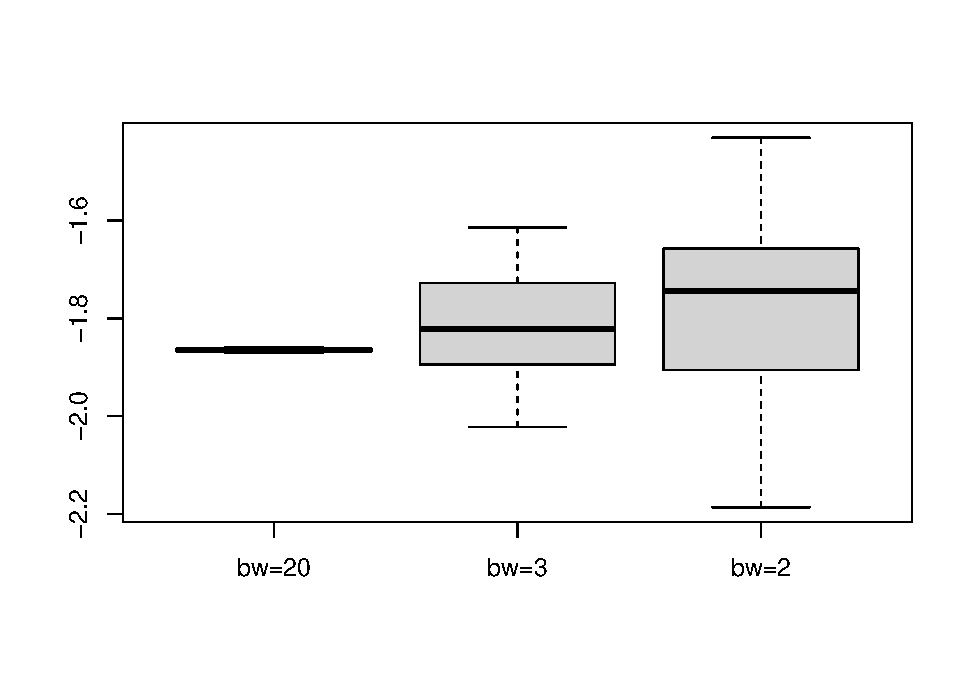
\includegraphics{modul_files/figure-latex/unnamed-chunk-80-1.pdf}

Output di atas memperlihatkan bahwa bandwidth yang lebih besar cenderung menghasilkan penduga koefisien model dengan rentang nilai yang lebih sempit. Sebaliknya, jika bandwidth yang digunakan lebih kecil, maka penduga koefisien model cenderung memiliki rentang nilai yang lebih lebar.

\hypertarget{menentukan-bandwidth-optimal}{%
\section{Menentukan Bandwidth Optimal}\label{menentukan-bandwidth-optimal}}

Penentuan bandwidth yang optimal dapat ditentukan berdasarkan kriteria AIC atau CV. Selain itu, kita juga dapat memilih fungsi pembobot kernel yang ingin digunakan pada pemodelan GWR.

\begin{Shaded}
\begin{Highlighting}[]
\NormalTok{bw1 }\OtherTok{\textless{}{-}} \FunctionTok{gwr.sel}\NormalTok{(Kemiskinan}\SpecialCharTok{\textasciitilde{}}\NormalTok{Rata.Rata.Lama.Sekolah,}\AttributeTok{data=}\NormalTok{datajawa) }\CommentTok{\# default method is CV}
\end{Highlighting}
\end{Shaded}

\begin{verbatim}
## Bandwidth: 3.450257 CV score: 946.7623 
## Bandwidth: 5.577059 CV score: 985.8033 
## Bandwidth: 2.135821 CV score: 877.1735 
## Bandwidth: 1.323454 CV score: 806.2682 
## Bandwidth: 0.8213845 CV score: 752.5299 
## Bandwidth: 0.5110882 CV score: 697.962 
## Bandwidth: 0.3193146 CV score: 699.4435 
## Bandwidth: 0.4257648 CV score: 686.988 
## Bandwidth: 0.4182171 CV score: 686.7128 
## Bandwidth: 0.4036248 CV score: 686.6801 
## Bandwidth: 0.3714212 CV score: 689.1402 
## Bandwidth: 0.4101954 CV score: 686.6098 
## Bandwidth: 0.4102361 CV score: 686.6098 
## Bandwidth: 0.4101547 CV score: 686.6098 
## Bandwidth: 0.4076605 CV score: 686.62 
## Bandwidth: 0.410114 CV score: 686.6098 
## Bandwidth: 0.4101547 CV score: 686.6098
\end{verbatim}

\begin{Shaded}
\begin{Highlighting}[]
\NormalTok{gwr01 }\OtherTok{\textless{}{-}} \FunctionTok{gwr}\NormalTok{(Kemiskinan}\SpecialCharTok{\textasciitilde{}}\NormalTok{Rata.Rata.Lama.Sekolah,}\AttributeTok{data=}\NormalTok{datajawa,}\AttributeTok{bandwidth=}\NormalTok{bw1)}

\NormalTok{bw2 }\OtherTok{\textless{}{-}} \FunctionTok{gwr.sel}\NormalTok{(Kemiskinan}\SpecialCharTok{\textasciitilde{}}\NormalTok{Rata.Rata.Lama.Sekolah,}\AttributeTok{data=}\NormalTok{datajawa,}\AttributeTok{method=}\StringTok{"aic"}\NormalTok{)}
\end{Highlighting}
\end{Shaded}

\begin{verbatim}
## Bandwidth: 3.450257 AIC: 587.2351 
## Bandwidth: 5.577059 AIC: 591.8688 
## Bandwidth: 2.135821 AIC: 578.5693 
## Bandwidth: 1.323454 AIC: 569.3341 
## Bandwidth: 0.8213845 AIC: 562.5431 
## Bandwidth: 0.5110882 AIC: 558.7068 
## Bandwidth: 0.3193146 AIC: 575.363 
## Bandwidth: 0.6296109 AIC: 559.226 
## Bandwidth: 0.5177358 AIC: 558.6444 
## Bandwidth: 0.5525482 AIC: 558.5357 
## Bandwidth: 0.5819835 AIC: 558.6792 
## Bandwidth: 0.547683 AIC: 558.531 
## Bandwidth: 0.5465411 AIC: 558.5307 
## Bandwidth: 0.5462381 AIC: 558.5307 
## Bandwidth: 0.5462788 AIC: 558.5307 
## Bandwidth: 0.5461974 AIC: 558.5307 
## Bandwidth: 0.5462381 AIC: 558.5307
\end{verbatim}

\begin{Shaded}
\begin{Highlighting}[]
\NormalTok{gwr02 }\OtherTok{\textless{}{-}} \FunctionTok{gwr}\NormalTok{(Kemiskinan}\SpecialCharTok{\textasciitilde{}}\NormalTok{Rata.Rata.Lama.Sekolah,}\AttributeTok{data=}\NormalTok{datajawa,}\AttributeTok{bandwidth=}\NormalTok{bw2)}

\NormalTok{bwbs1 }\OtherTok{\textless{}{-}} \FunctionTok{gwr.sel}\NormalTok{(Kemiskinan}\SpecialCharTok{\textasciitilde{}}\NormalTok{Rata.Rata.Lama.Sekolah,}\AttributeTok{data=}\NormalTok{datajawa,}\AttributeTok{gweight=}\NormalTok{gwr.bisquare)}
\end{Highlighting}
\end{Shaded}

\begin{verbatim}
## Bandwidth: 3.450257 CV score: 816.2604 
## Bandwidth: 5.577059 CV score: 893.215 
## Bandwidth: 2.135821 CV score: 765.5706 
## Bandwidth: 1.323454 CV score: 696.4003 
## Bandwidth: 0.8213845 CV score: 722.8235 
## Bandwidth: 1.323495 CV score: 696.395 
## Bandwidth: 1.633776 CV score: 719.824 
## Bandwidth: 1.421531 CV score: 697.7054 
## Bandwidth: 1.36793 CV score: 694.5978 
## Bandwidth: 1.355794 CV score: 694.4734 
## Bandwidth: 1.358597 CV score: 694.4715 
## Bandwidth: 1.357479 CV score: 694.4699 
## Bandwidth: 1.357438 CV score: 694.4699 
## Bandwidth: 1.357397 CV score: 694.4699 
## Bandwidth: 1.357438 CV score: 694.4699
\end{verbatim}

\begin{Shaded}
\begin{Highlighting}[]
\NormalTok{gwr03 }\OtherTok{\textless{}{-}} \FunctionTok{gwr}\NormalTok{(Kemiskinan}\SpecialCharTok{\textasciitilde{}}\NormalTok{Rata.Rata.Lama.Sekolah,}\AttributeTok{data=}\NormalTok{datajawa,}\AttributeTok{gweight=}\NormalTok{gwr.bisquare,}
    \AttributeTok{bandwidth=}\NormalTok{bwbs1)}

\NormalTok{bwbs2 }\OtherTok{\textless{}{-}} \FunctionTok{gwr.sel}\NormalTok{(Kemiskinan}\SpecialCharTok{\textasciitilde{}}\NormalTok{Rata.Rata.Lama.Sekolah,}\AttributeTok{data=}\NormalTok{datajawa,}
                 \AttributeTok{gweight=}\NormalTok{gwr.bisquare,}\AttributeTok{method=}\StringTok{"aic"}\NormalTok{)}
\end{Highlighting}
\end{Shaded}

\begin{verbatim}
## Bandwidth: 3.450257 AIC: 570.608 
## Bandwidth: 5.577059 AIC: 580.6548 
## Bandwidth: 2.135821 AIC: 564.1267 
## Bandwidth: 1.323454 AIC: 558.0575 
## Bandwidth: 0.8213845 AIC: 575.6082 
## Bandwidth: 1.633751 AIC: 558.9865 
## Bandwidth: 1.310745 AIC: 558.1617 
## Bandwidth: 1.435388 AIC: 557.6479 
## Bandwidth: 1.429706 AIC: 557.6416 
## Bandwidth: 1.420138 AIC: 557.6375 
## Bandwidth: 1.420321 AIC: 557.6375 
## Bandwidth: 1.420399 AIC: 557.6375 
## Bandwidth: 1.42044 AIC: 557.6375 
## Bandwidth: 1.420399 AIC: 557.6375
\end{verbatim}

\begin{Shaded}
\begin{Highlighting}[]
\NormalTok{gwr04 }\OtherTok{\textless{}{-}} \FunctionTok{gwr}\NormalTok{(Kemiskinan}\SpecialCharTok{\textasciitilde{}}\NormalTok{Rata.Rata.Lama.Sekolah,}\AttributeTok{data=}\NormalTok{datajawa,}\AttributeTok{gweight=}\NormalTok{gwr.bisquare,}
    \AttributeTok{bandwidth=}\NormalTok{bwbs2)}
\end{Highlighting}
\end{Shaded}

\hypertarget{menentukan-model-terbaik}{%
\section{Menentukan Model Terbaik}\label{menentukan-model-terbaik}}

Penentuan model terbaik dapat ditentukan berdasarkan beberapa kriteria tertentu. Fungsi \texttt{gwr} memungkinkan kita untuk mengevaluasi model berdasarkan AIC dan global quasi-\(R^2\), dengan terlebih dulu menambahkan argumen \texttt{hatmatrix=TRUE}.

\begin{Shaded}
\begin{Highlighting}[]
\NormalTok{gwr01 }\OtherTok{\textless{}{-}} \FunctionTok{gwr}\NormalTok{(Kemiskinan}\SpecialCharTok{\textasciitilde{}}\NormalTok{Rata.Rata.Lama.Sekolah,}\AttributeTok{data=}\NormalTok{datajawa,}
             \AttributeTok{hatmatrix=}\NormalTok{T, }\AttributeTok{bandwidth=}\NormalTok{bw1)}
\NormalTok{gwr01}
\end{Highlighting}
\end{Shaded}

\begin{verbatim}
## Call:
## gwr(formula = Kemiskinan ~ Rata.Rata.Lama.Sekolah, data = datajawa, 
##     bandwidth = bw1, hatmatrix = T)
## Kernel function: gwr.Gauss 
## Fixed bandwidth: 0.4101547 
## Summary of GWR coefficient estimates at data points:
##                            Min.  1st Qu.   Median  3rd Qu.     Max.  Global
## X.Intercept.           12.68449 18.33784 23.15972 26.20076 38.10046 24.7340
## Rata.Rata.Lama.Sekolah -4.20789 -2.05946 -1.55904 -1.22414 -0.46292 -1.8657
## Number of data points: 119 
## Effective number of parameters (residual: 2traceS - traceS'S): 34.33575 
## Effective degrees of freedom (residual: 2traceS - traceS'S): 84.66425 
## Sigma (residual: 2traceS - traceS'S): 2.291766 
## Effective number of parameters (model: traceS): 25.10699 
## Effective degrees of freedom (model: traceS): 93.89301 
## Sigma (model: traceS): 2.176225 
## Sigma (ML): 1.933067 
## AICc (GWR p. 61, eq 2.33; p. 96, eq. 4.21): 562.1913 
## AIC (GWR p. 96, eq. 4.22): 519.682 
## Residual sum of squares: 444.673 
## Quasi-global R2: 0.7874434
\end{verbatim}

Fungsi \texttt{gwr} memberikan nilai AIC dengan tiga pendekatan, sehingga kita memperoleh AICc, AICb, dan AICh.

\begin{Shaded}
\begin{Highlighting}[]
\NormalTok{gwr01}\SpecialCharTok{$}\NormalTok{results}\SpecialCharTok{$}\NormalTok{AICc}
\end{Highlighting}
\end{Shaded}

\begin{verbatim}
## [1] 569.1585
\end{verbatim}

\begin{Shaded}
\begin{Highlighting}[]
\NormalTok{gwr01}\SpecialCharTok{$}\NormalTok{results}\SpecialCharTok{$}\NormalTok{AICb}
\end{Highlighting}
\end{Shaded}

\begin{verbatim}
## [1] 562.1913
\end{verbatim}

\begin{Shaded}
\begin{Highlighting}[]
\NormalTok{gwr01}\SpecialCharTok{$}\NormalTok{results}\SpecialCharTok{$}\NormalTok{AICh}
\end{Highlighting}
\end{Shaded}

\begin{verbatim}
## [1] 519.682
\end{verbatim}

Model terbaik adalah yang memiliki nilai AIC terkecil (bisa juga negatif) dan nilai global quasi-\(R^2\) yang terbesar. Namun demikian, kriteria tersebut tidak memberikan informasi inferensia apapun terkait siginifikansi model GWR.

Beberapa pendekatan uji dapat dilakukan untuk menguji \(H_0\) yang menyatakan bahwa model GWR tidak lebih baik daripada model OLS (regresi linier klasik), seperti yang dapat dilihat pada program-program berikut ini.

\begin{Shaded}
\begin{Highlighting}[]
\FunctionTok{BFC02.gwr.test}\NormalTok{(gwr01)}
\end{Highlighting}
\end{Shaded}

\begin{verbatim}
## 
##  Brunsdon, Fotheringham & Charlton (2002, pp. 91-2) ANOVA
## 
## data:  gwr01
## F = 2.2103, df1 = 117.000, df2 = 84.664, p-value = 7.714e-05
## alternative hypothesis: greater
## sample estimates:
## SS OLS residuals SS GWR residuals 
##         982.8726         444.6730
\end{verbatim}

\begin{Shaded}
\begin{Highlighting}[]
\FunctionTok{BFC99.gwr.test}\NormalTok{(gwr01)}
\end{Highlighting}
\end{Shaded}

\begin{verbatim}
## 
##  Brunsdon, Fotheringham & Charlton (1999) ANOVA
## 
## data:  gwr01
## F = 3.169, df1 = 87.18, df2 = 96.67, p-value = 2.996e-08
## alternative hypothesis: greater
## sample estimates:
## SS GWR improvement   SS GWR residuals 
##           538.1996           444.6730
\end{verbatim}

\begin{Shaded}
\begin{Highlighting}[]
\FunctionTok{LMZ.F1GWR.test}\NormalTok{(gwr01)}
\end{Highlighting}
\end{Shaded}

\begin{verbatim}
## 
##  Leung et al. (2000) F(1) test
## 
## data:  gwr01
## F = 0.62521, df1 = 96.67, df2 = 117.00, p-value = 0.00875
## alternative hypothesis: less
## sample estimates:
## SS OLS residuals SS GWR residuals 
##         982.8726         444.6730
\end{verbatim}

\begin{Shaded}
\begin{Highlighting}[]
\FunctionTok{LMZ.F2GWR.test}\NormalTok{(gwr01)}
\end{Highlighting}
\end{Shaded}

\begin{verbatim}
## 
##  Leung et al. (2000) F(2) test
## 
## data:  gwr01
## F = 1.9813, df1 = 47.916, df2 = 117.000, p-value = 0.001549
## alternative hypothesis: greater
## sample estimates:
##   SS OLS residuals SS GWR improvement 
##           982.8726           538.1996
\end{verbatim}

Berdasarkan output di atas, seluruh uji menunjukkan nilai \(p\)-value yang lebih kecil daripada taraf nyata 0.05, artinya \(H_0\) dapat ditolak, dan kita dapat menyimpulkan bahwa model GWR lebih baik daripada OLS, pada taraf nyata 5\%.

\begin{Shaded}
\begin{Highlighting}[]
\FunctionTok{LMZ.F3GWR.test}\NormalTok{(gwr01)}
\end{Highlighting}
\end{Shaded}

\begin{verbatim}
## 
## Leung et al. (2000) F(3) test
## 
##                        F statistic Numerator d.f. Denominator d.f.     Pr(>)
## (Intercept)                 2.6985        46.6539            96.67 1.988e-05
## Rata.Rata.Lama.Sekolah      2.1191        25.3140            96.67  0.004783
##                           
## (Intercept)            ***
## Rata.Rata.Lama.Sekolah ** 
## ---
## Signif. codes:  0 '***' 0.001 '**' 0.01 '*' 0.05 '.' 0.1 ' ' 1
\end{verbatim}

\hypertarget{menginterpretasikan-hasil-pemodelan-gwr}{%
\section{Menginterpretasikan Hasil Pemodelan GWR}\label{menginterpretasikan-hasil-pemodelan-gwr}}

Koefisien model GWR bersifat lokal, sehingga nilai penduga koefisien akan diperoleh pada setiap titik pengamatan. Oleh karenanya, interpretasi model GWR seringkali dilakukan dengan membuat visualisasi dalam bentuk peta, baru kemudian menginterpretasikannya.

\begin{Shaded}
\begin{Highlighting}[]
\FunctionTok{str}\NormalTok{(gwr01}\SpecialCharTok{$}\NormalTok{SDF)}
\end{Highlighting}
\end{Shaded}

\begin{verbatim}
## Formal class 'SpatialPointsDataFrame' [package "sp"] with 5 slots
##   ..@ data       :'data.frame':  119 obs. of  12 variables:
##   .. ..$ sum.w                        : num [1:119] 7.49 14.3 13.86 13.78 13.72 ...
##   .. ..$ (Intercept)                  : num [1:119] 17.1 15.5 15.8 15.8 15.7 ...
##   .. ..$ Rata.Rata.Lama.Sekolah       : num [1:119] -1.21 -1.08 -1.11 -1.1 -1.09 ...
##   .. ..$ (Intercept)_se               : num [1:119] 3.52 2.76 2.79 2.83 2.85 ...
##   .. ..$ Rata.Rata.Lama.Sekolah_se    : num [1:119] 0.35 0.287 0.29 0.294 0.295 ...
##   .. ..$ gwr.e                        : num [1:119] 5.168 -0.198 0.191 0.206 -0.93 ...
##   .. ..$ pred                         : num [1:119] 6.81 3.03 2.95 3.38 4.32 ...
##   .. ..$ pred.se                      : num [1:119] 0.761 0.775 0.794 0.708 0.554 ...
##   .. ..$ localR2                      : num [1:119] 0.485 0.633 0.642 0.616 0.602 ...
##   .. ..$ (Intercept)_se_EDF           : num [1:119] 3.71 2.91 2.94 2.98 3 ...
##   .. ..$ Rata.Rata.Lama.Sekolah_se_EDF: num [1:119] 0.369 0.303 0.306 0.309 0.311 ...
##   .. ..$ pred.se                      : num [1:119] 0.801 0.816 0.836 0.746 0.583 ...
##   ..@ coords.nrs : num(0) 
##   ..@ coords     : num [1:119, 1:2] 107 107 107 107 107 ...
##   .. ..- attr(*, "dimnames")=List of 2
##   .. .. ..$ : chr [1:119] "1" "2" "3" "4" ...
##   .. .. ..$ : chr [1:2] "Longitude" "Latitude"
##   ..@ bbox       : num [1:2, 1:2] 105.69 -8.24 114.37 -5.8
##   .. ..- attr(*, "dimnames")=List of 2
##   .. .. ..$ : chr [1:2] "Longitude" "Latitude"
##   .. .. ..$ : chr [1:2] "min" "max"
##   ..@ proj4string:Formal class 'CRS' [package "sp"] with 1 slot
##   .. .. ..@ projargs: chr NA
\end{verbatim}

Beberapa nilai dapat diperoleh langsung dari output fungsi \texttt{gwr}, yaitu penduga koefisien, hasil prediksi model, serta \emph{local}-\(R^2\). Selanjutnya, interpretasi dapat disesuaikan dengan konteks penelitian.

\begin{Shaded}
\begin{Highlighting}[]
\NormalTok{petajawa}\SpecialCharTok{$}\NormalTok{beta}\OtherTok{\textless{}{-}}\NormalTok{gwr01}\SpecialCharTok{$}\NormalTok{SDF}\SpecialCharTok{$}\NormalTok{Rata.Rata.Lama.Sekolah}
\NormalTok{petajawa}\SpecialCharTok{$}\NormalTok{pred}\OtherTok{\textless{}{-}}\NormalTok{gwr01}\SpecialCharTok{$}\NormalTok{SDF}\SpecialCharTok{$}\NormalTok{pred}
\NormalTok{petajawa}\SpecialCharTok{$}\NormalTok{localR2}\OtherTok{\textless{}{-}}\NormalTok{gwr01}\SpecialCharTok{$}\NormalTok{SDF}\SpecialCharTok{$}\NormalTok{localR2}

\FunctionTok{spplot}\NormalTok{(petajawa, }\StringTok{"beta"}\NormalTok{, }\AttributeTok{main=}\StringTok{"Penduga Koefisien Model GWR"}\NormalTok{)}
\end{Highlighting}
\end{Shaded}

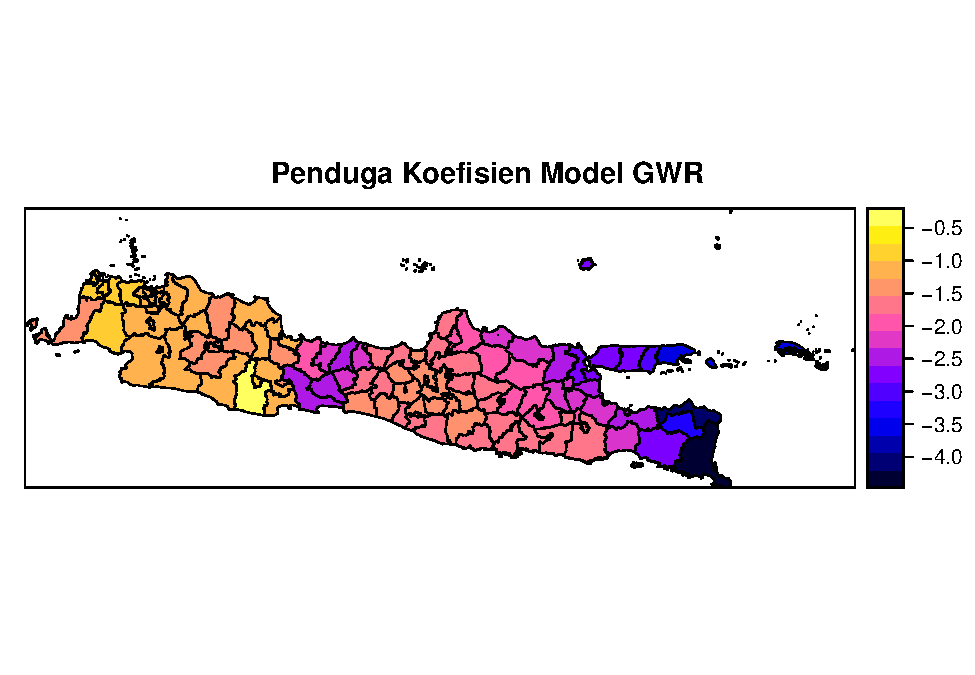
\includegraphics{modul_files/figure-latex/unnamed-chunk-90-1.pdf}

\begin{Shaded}
\begin{Highlighting}[]
\FunctionTok{spplot}\NormalTok{(petajawa, }\StringTok{"pred"}\NormalTok{, }\AttributeTok{main=}\StringTok{"Prediksi Kemiskinan"}\NormalTok{)}
\end{Highlighting}
\end{Shaded}

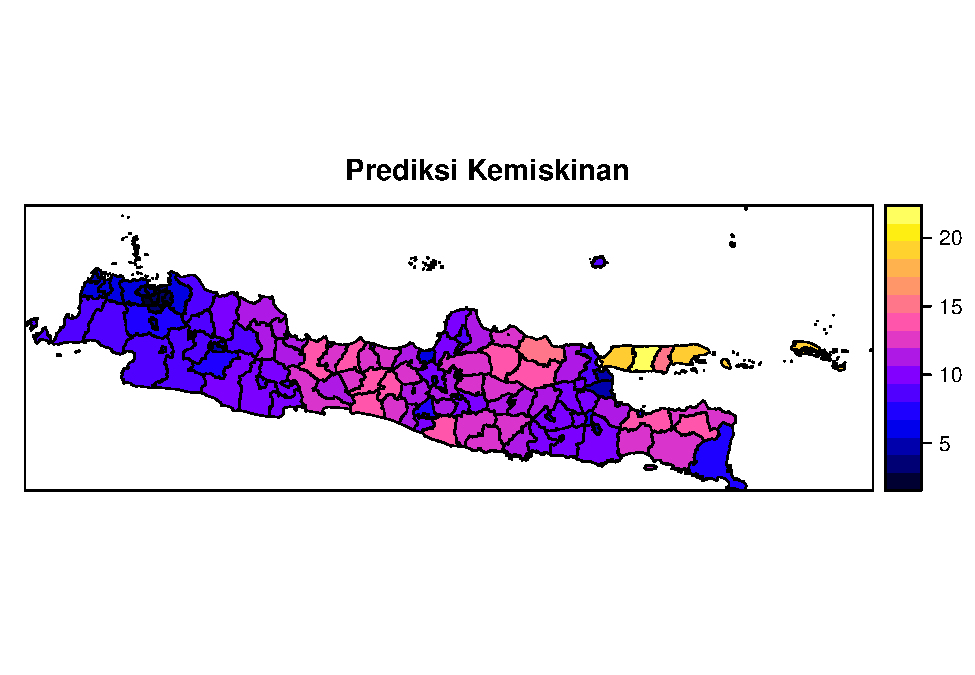
\includegraphics{modul_files/figure-latex/unnamed-chunk-90-2.pdf}

\begin{Shaded}
\begin{Highlighting}[]
\FunctionTok{spplot}\NormalTok{(petajawa, }\StringTok{"localR2"}\NormalTok{, }\AttributeTok{main=}\StringTok{"Local R{-}square"}\NormalTok{)}
\end{Highlighting}
\end{Shaded}

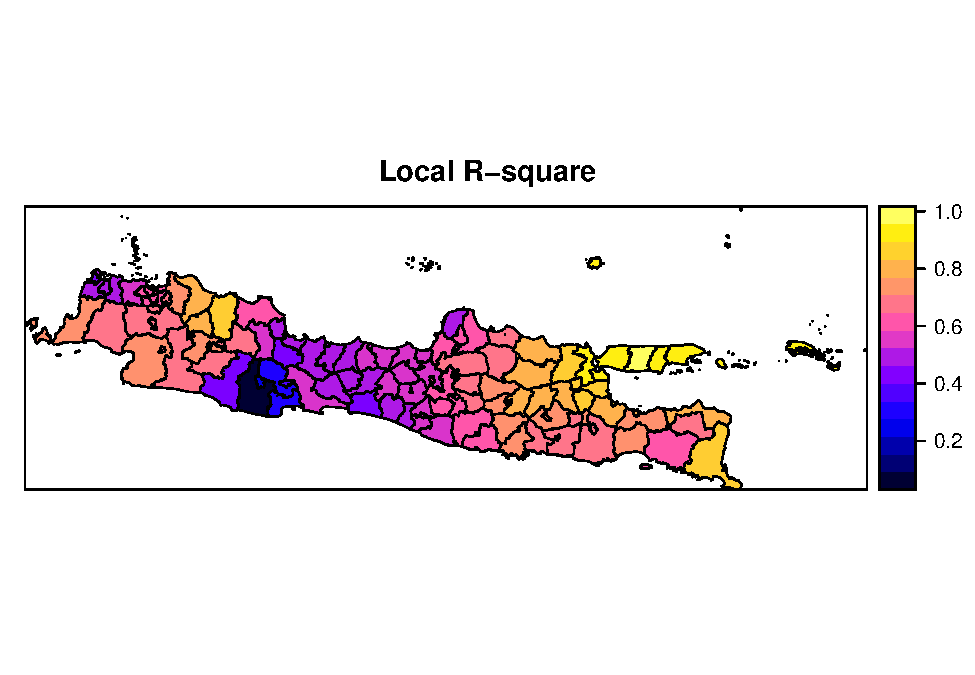
\includegraphics{modul_files/figure-latex/unnamed-chunk-90-3.pdf}

\hypertarget{sumber-pustaka-2}{%
\section{Sumber Pustaka}\label{sumber-pustaka-2}}

Brazil, N. (n.d.). Geographically weighted regression. CRD 230: Spatial Methods in Community Research. \url{https://crd230.github.io/gwr.html\#ordinary_least_squares_regression}

Brunsdon, C. 2015. Geographically Weighted Regression. \url{https://rstudio-pubs-static.s3.amazonaws.com/176883_06a3fa1fc77444be85e94dcd97ba9a34.html}

Dennett, A. (2014, November 17). An introduction to geographically weighted regression in R. \url{https://rstudio-pubs-static.s3.amazonaws.com/44975_0342ec49f925426fa16ebcdc28210118.html}

\hypertarget{regresi-data-panel-spasial}{%
\chapter{Regresi Data Panel Spasial}\label{regresi-data-panel-spasial}}

Pemodelan ini merupakan salah satu alternatif yang dapat dilakukan ketika data yang kita kaji selain merupakan data spasial, juga merupakan data deret waktu.

Tahapan yang dapat dilakukan dalam melakukan pemodelan regresi data panel adalah sebagai berikut:

\begin{enumerate}
\def\labelenumi{(\arabic{enumi})}
\item
  melakukan eksplorasi hubungan antar peubah, sebaran data, dsb.
\item
  menganalisa data panel dengan melakukan pengujian berikut:

  \begin{itemize}
  \item
    Uji Breusch-Pagan untuk menguji adanya efek waktu, individu atau keduanya
  \item
    Uji Chow untuk menguji signifikansi antara model gabungan dan model pengaruh tetap
  \item
    Uji Hausman untuk menguji signifikansi antara model pengaruh acak dengan model pengaruh tetap
  \end{itemize}
\item
  melakukan pemodelan data panel sesuai dengan indikasi yang diperoleh pada tahap (1) s.d (3)
\item
  mengevaluasi kebaikan model
\end{enumerate}

Sedangkan tahapan dalam pemodelan data panel spasial adalah: (Rakhmi, 2015)

\begin{enumerate}
\def\labelenumi{(\arabic{enumi})}
\item
  Eksplorasi Data
\item
  Uji ketergantungan spasial, dapat menggunakan uji CD Pesaran dengan hipotesis sebagai berikut:
\end{enumerate}

\begin{quote}
\(H_0: \rho_{ij}=\rho_{ji}= korelasi(\varepsilon_{it}, \varepsilon_{jt})=0\), untuk \(i \ne j\)
\end{quote}

\begin{quote}
\(H_1: \rho_{ij}=\rho_{ji} \ne 0\) , untuk beberapa \(i \ne j\)
\end{quote}

\begin{enumerate}
\def\labelenumi{(\arabic{enumi})}
\setcounter{enumi}{2}
\item
  Bila perlu, menguji autokorelasi spasial pada peubah penjelas, dapat menggunakan uji Moran.
\item
  Sesuai dengan indikasi pada tahapan sebelumnya, kita dapat melakukan pemodelan data panel spasial, dengan menggunakan matriks pembobot spasial yang sesuai.
\item
  Mengevaluasi kebaikan model yang disusun pada tahap (4).
\item
  Menginterpretasikan model.
\end{enumerate}

\hypertarget{ilustrasi-kemiskinan-di-pulau-jawa}{%
\section{Ilustrasi: Kemiskinan di Pulau Jawa}\label{ilustrasi-kemiskinan-di-pulau-jawa}}

Sebagai ilustrasi, modul ini akan membahas studi kasus yang diteliti oleh Agusti (2015). Pada ilustrasi ini, kita akan mengamati persentasi kemiskinan di kabupaten dan kota di Pulau Jawa pada tahun 2008-2012, dengan rincian peubah sebagai berikut:

\begin{itemize}
\item
  Y = Persentase Kemiskinan di kabupaten/kota di Pulau Jawa
\item
  X1 = Indeks Pembangunan Manusia (IPM)
\item
  X2 = Tingkat Pengangguran Terbuka (TPT)
\item
  X3 = Pertumbuhan Ekonomi (PDRB)
\end{itemize}

Pertama-tama, kita impor data peta tematik pulau Jawa dan data pengamatan ke dalam R.

\begin{Shaded}
\begin{Highlighting}[]
\NormalTok{data}\OtherTok{\textless{}{-}}\FunctionTok{read.csv}\NormalTok{(}\StringTok{"data panel Jawa.csv"}\NormalTok{, }\AttributeTok{header =}\NormalTok{ T)}
\FunctionTok{head}\NormalTok{(data)}
\end{Highlighting}
\end{Shaded}

\begin{verbatim}
##     Id    Provinsi                KabKot Tahun Kemiskinan   IPM   PDRB   TPT
## 1 3101 DKI JAKARTA           Kep. Seribu  2008      13.56 70.14   3.45 11.67
## 2 3101 DKI JAKARTA           Kep. Seribu  2009      12.66 70.50   3.48 11.57
## 3 3101 DKI JAKARTA           Kep. Seribu  2010      13.01 70.82   4.06  9.89
## 4 3101 DKI JAKARTA           Kep. Seribu  2011      11.53 71.16   5.34 11.38
## 5 3101 DKI JAKARTA           Kep. Seribu  2012      11.62 71.45   5.63 13.97
## 6 3171 DKI JAKARTA  Kota Jakarta Selatan  2008       3.41 79.00 152.15 11.96
\end{verbatim}

\hypertarget{eksplorasi-data-2}{%
\section{Eksplorasi Data}\label{eksplorasi-data-2}}

\begin{Shaded}
\begin{Highlighting}[]
\NormalTok{y}\OtherTok{\textless{}{-}}\FunctionTok{matrix}\NormalTok{(}\ConstantTok{NA}\NormalTok{, }\AttributeTok{nrow=}\DecValTok{5}\NormalTok{, }\AttributeTok{ncol=}\DecValTok{119}\NormalTok{) }\CommentTok{\# 5 tahun, 118 kota/kabupaten}
\NormalTok{y[,}\DecValTok{1}\NormalTok{]}\OtherTok{\textless{}{-}}\DecValTok{2008}\SpecialCharTok{:}\DecValTok{2012}
\NormalTok{a}\OtherTok{=}\DecValTok{2}
\ControlFlowTok{for}\NormalTok{ (i }\ControlFlowTok{in} \DecValTok{1}\SpecialCharTok{:}\DecValTok{118}\NormalTok{)}
\NormalTok{\{}
\NormalTok{  y[,i}\SpecialCharTok{+}\DecValTok{1}\NormalTok{]}\OtherTok{\textless{}{-}}\NormalTok{data[a}\SpecialCharTok{:}\NormalTok{(a}\SpecialCharTok{+}\DecValTok{4}\NormalTok{),}\DecValTok{5}\NormalTok{]}
\NormalTok{  a}\OtherTok{=}\NormalTok{a}\SpecialCharTok{+}\DecValTok{5}
\NormalTok{\}}

\FunctionTok{palette}\NormalTok{(}\StringTok{"default"}\NormalTok{)}
\NormalTok{y}\OtherTok{\textless{}{-}}\FunctionTok{as.data.frame}\NormalTok{(y)}
\FunctionTok{matplot}\NormalTok{(y[,}\DecValTok{1}\NormalTok{], y[,}\SpecialCharTok{{-}}\DecValTok{1}\NormalTok{], }\AttributeTok{type=}\StringTok{"l"}\NormalTok{, }\AttributeTok{pch=}\DecValTok{19}\NormalTok{, }\AttributeTok{ylab=}\StringTok{"Persentase Kemiskinan"}\NormalTok{, }\AttributeTok{xlab=}\StringTok{"Tahun"}\NormalTok{)}
\end{Highlighting}
\end{Shaded}

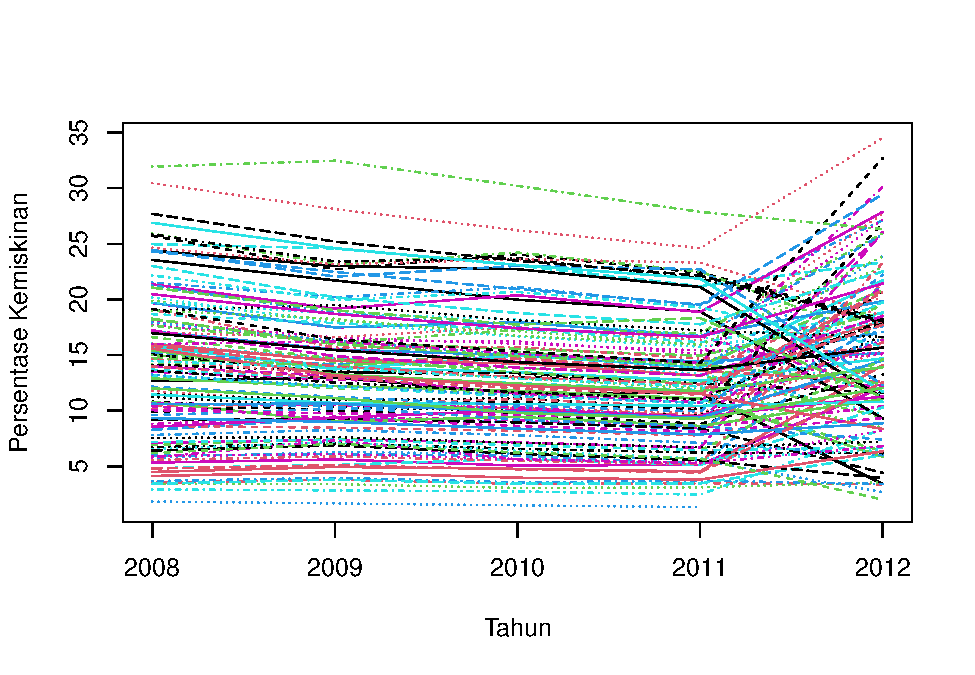
\includegraphics{modul_files/figure-latex/unnamed-chunk-92-1.pdf}

\begin{Shaded}
\begin{Highlighting}[]
\CommentTok{\#install.packages("foreign")}
\FunctionTok{library}\NormalTok{(foreign)}

\NormalTok{data1}\OtherTok{\textless{}{-}}\FunctionTok{subset}\NormalTok{(data,data}\SpecialCharTok{$}\NormalTok{Provinsi}\SpecialCharTok{==}\StringTok{"DKI JAKARTA"}\NormalTok{)}
\FunctionTok{coplot}\NormalTok{(Kemiskinan}\SpecialCharTok{\textasciitilde{}}\NormalTok{Tahun}\SpecialCharTok{|}\NormalTok{KabKot, }\AttributeTok{type=}\StringTok{"l"}\NormalTok{, }\AttributeTok{data=}\NormalTok{data1)}
\end{Highlighting}
\end{Shaded}

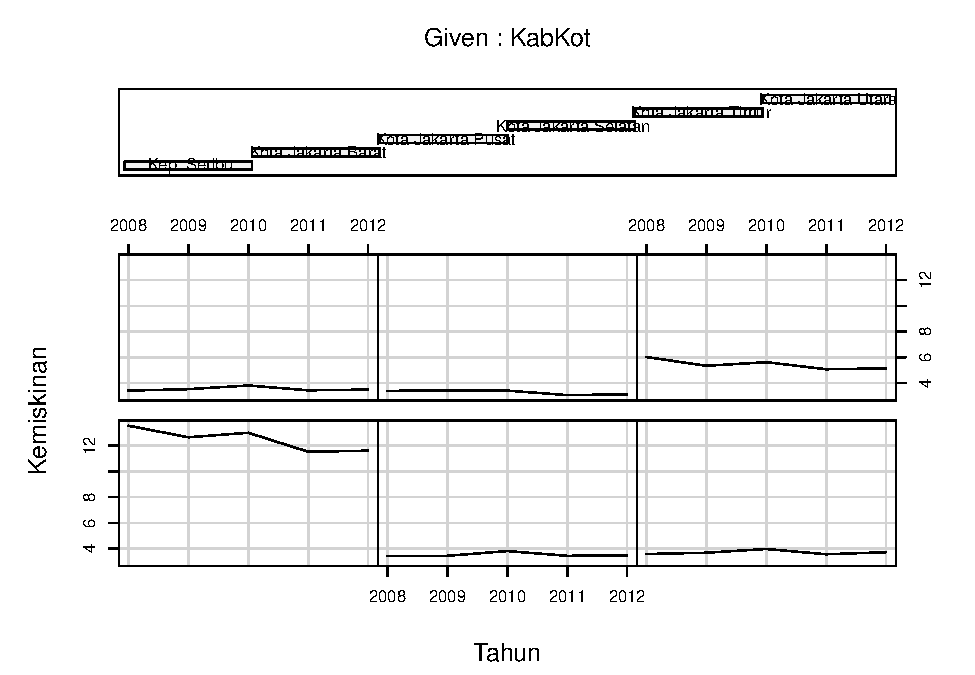
\includegraphics{modul_files/figure-latex/unnamed-chunk-93-1.pdf}

\begin{Shaded}
\begin{Highlighting}[]
\NormalTok{prov}\OtherTok{\textless{}{-}}\FunctionTok{unique}\NormalTok{(data}\SpecialCharTok{$}\NormalTok{Provinsi)}
\ControlFlowTok{for}\NormalTok{ (i }\ControlFlowTok{in} \DecValTok{1}\SpecialCharTok{:}\FunctionTok{length}\NormalTok{(prov))}
\NormalTok{\{}
\NormalTok{  data1}\OtherTok{\textless{}{-}}\FunctionTok{subset}\NormalTok{(data,data}\SpecialCharTok{$}\NormalTok{Provinsi}\SpecialCharTok{==}\NormalTok{prov[i])}
\NormalTok{  car}\SpecialCharTok{::}\FunctionTok{scatterplot}\NormalTok{(Kemiskinan}\SpecialCharTok{\textasciitilde{}}\NormalTok{Tahun}\SpecialCharTok{|}\NormalTok{KabKot, }\AttributeTok{boxplots=}\NormalTok{F, }\AttributeTok{smooth=}\NormalTok{F, }\AttributeTok{legend=}\NormalTok{F, }
                   \AttributeTok{grid=}\NormalTok{T,}\AttributeTok{data=}\NormalTok{data1, }\AttributeTok{reset.par=}\NormalTok{T, }\AttributeTok{cex=}\FloatTok{0.5}\NormalTok{, }\AttributeTok{main=}\NormalTok{prov[i])}
\NormalTok{\}}
\end{Highlighting}
\end{Shaded}

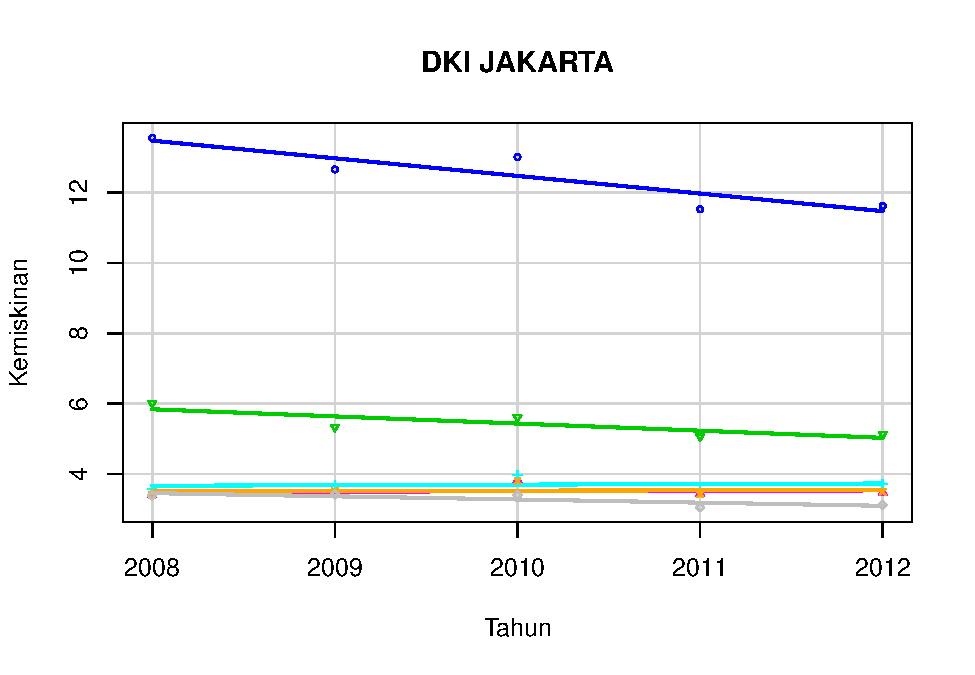
\includegraphics{modul_files/figure-latex/unnamed-chunk-94-1.pdf} 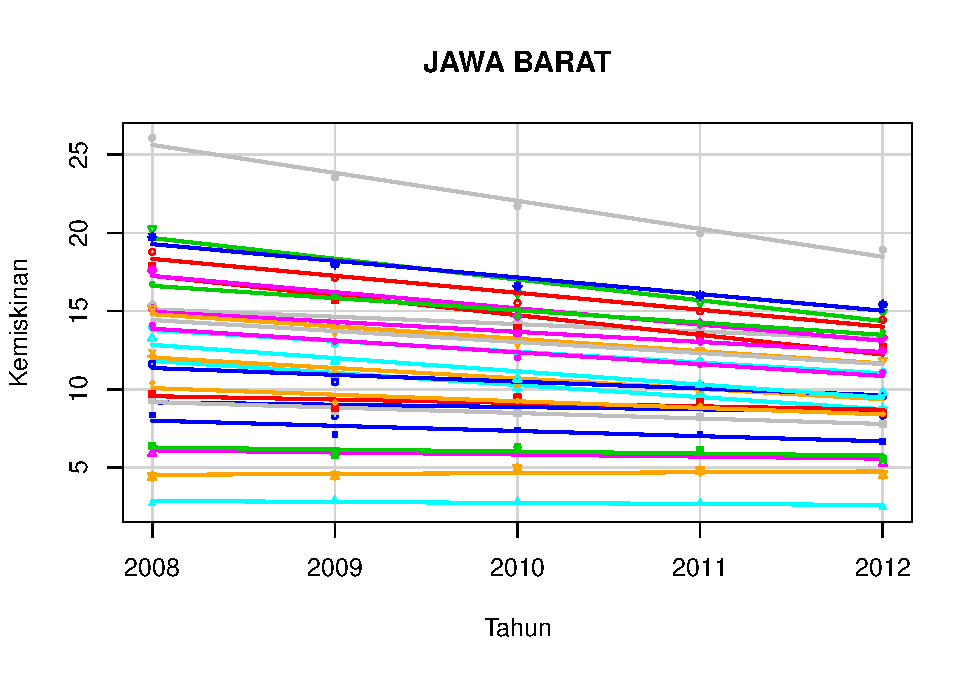
\includegraphics{modul_files/figure-latex/unnamed-chunk-94-2.pdf} 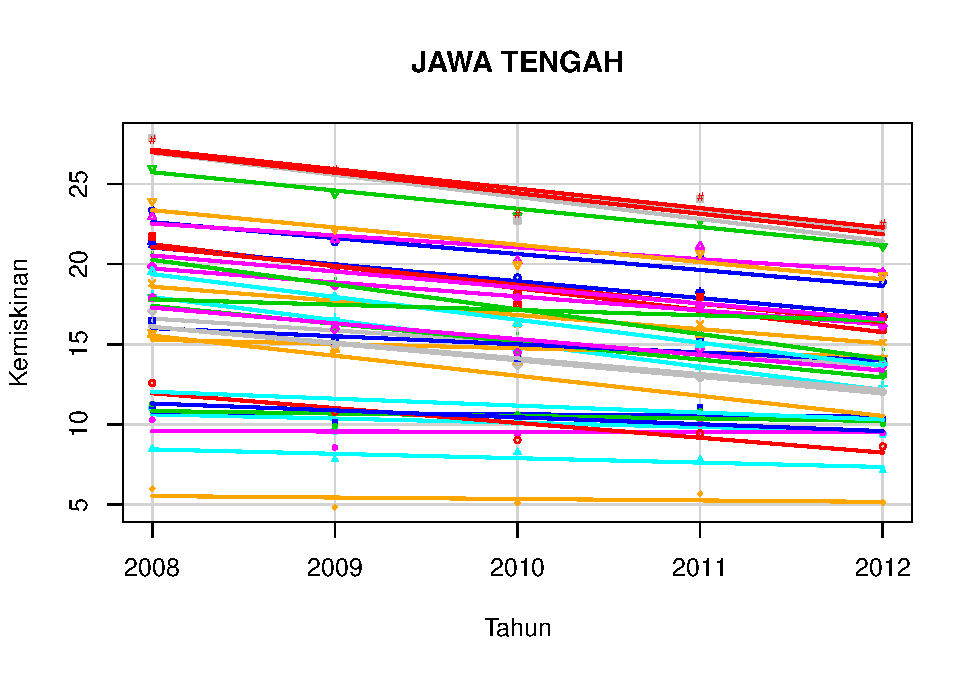
\includegraphics{modul_files/figure-latex/unnamed-chunk-94-3.pdf} 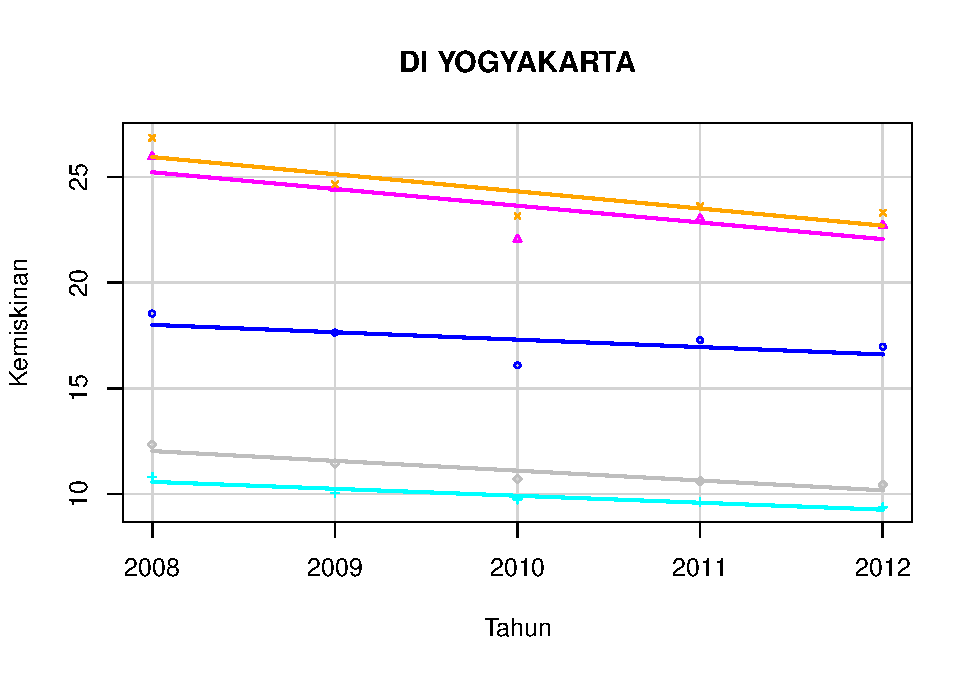
\includegraphics{modul_files/figure-latex/unnamed-chunk-94-4.pdf} 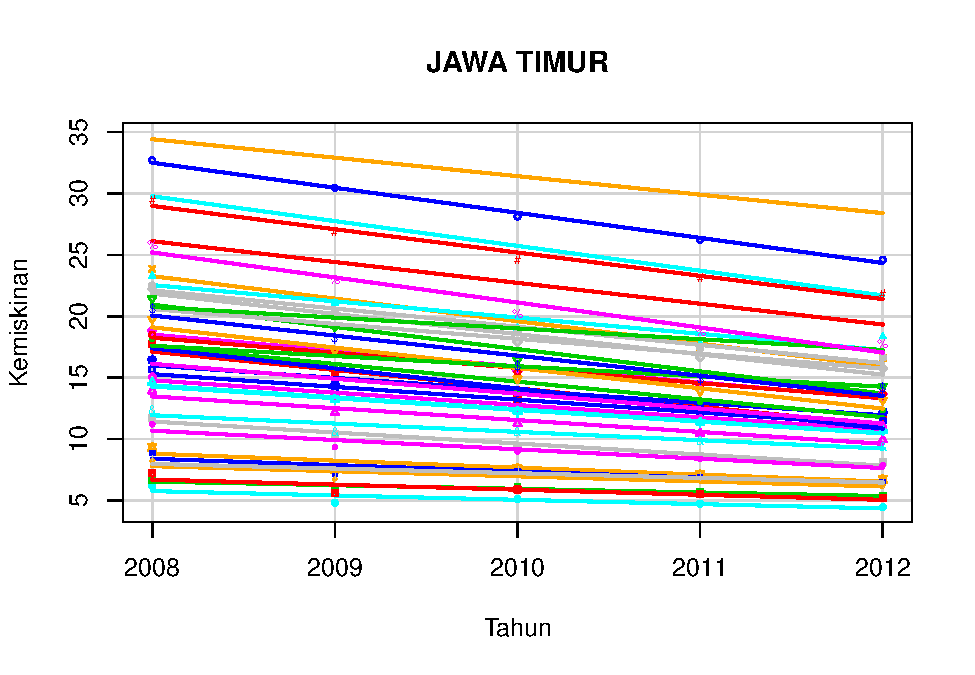
\includegraphics{modul_files/figure-latex/unnamed-chunk-94-5.pdf} 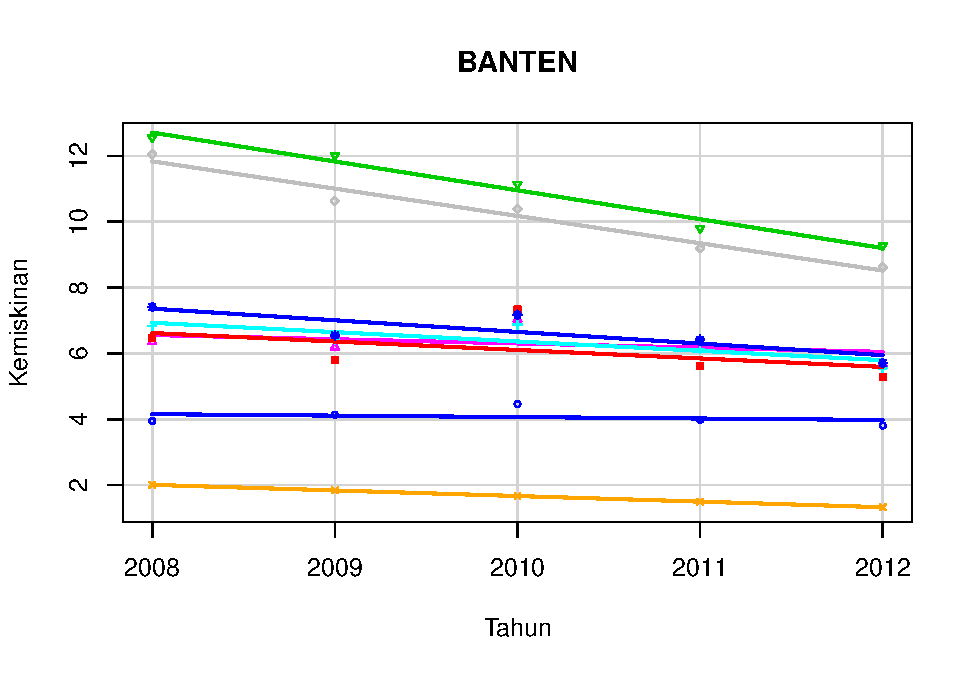
\includegraphics{modul_files/figure-latex/unnamed-chunk-94-6.pdf}

\begin{Shaded}
\begin{Highlighting}[]
\FunctionTok{plot}\NormalTok{(data[,}\DecValTok{5}\SpecialCharTok{:}\DecValTok{8}\NormalTok{], }\AttributeTok{pch=}\DecValTok{16}\NormalTok{, }\AttributeTok{col=}\StringTok{"blue"}\NormalTok{, }\AttributeTok{main=}\StringTok{"Scatterplot antar Pasangan Peubah pada 2008{-}2012"}\NormalTok{)}
\end{Highlighting}
\end{Shaded}

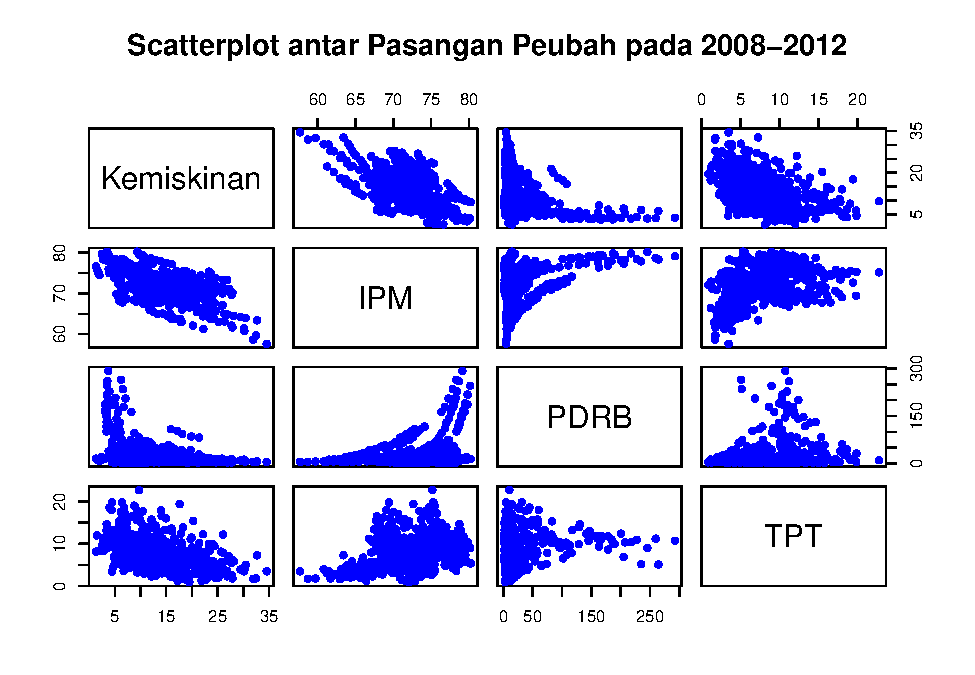
\includegraphics{modul_files/figure-latex/unnamed-chunk-95-1.pdf}

Scatterplot memperlihatkan bahwa IPM dan PDRB cenderung memiliki hubungan yang berbanding terbalik dengan persentase kemiskinan. Sedangkan pola hubungan antara persentase kemiskinan dengan peubah TPT memiliki ragam yang cukup besar sehingga agak sulit untuk mengidentifikasinya.

\begin{Shaded}
\begin{Highlighting}[]
\NormalTok{a}\OtherTok{=}\DecValTok{1}\NormalTok{; korelasipertahun}\OtherTok{\textless{}{-}}\ConstantTok{NULL}\NormalTok{;}
\ControlFlowTok{for}\NormalTok{ (i }\ControlFlowTok{in} \DecValTok{1}\SpecialCharTok{:}\DecValTok{5}\NormalTok{)}
\NormalTok{\{}
\NormalTok{  korelasi}\OtherTok{\textless{}{-}}\FunctionTok{cor}\NormalTok{(data[a}\SpecialCharTok{:}\NormalTok{(a}\SpecialCharTok{+}\DecValTok{4}\NormalTok{),}\DecValTok{5}\SpecialCharTok{:}\DecValTok{8}\NormalTok{])[}\SpecialCharTok{{-}}\DecValTok{1}\NormalTok{,}\DecValTok{1}\NormalTok{]}
\NormalTok{  a}\OtherTok{=}\NormalTok{a}\SpecialCharTok{+}\DecValTok{5}
\NormalTok{  korelasipertahun}\OtherTok{\textless{}{-}}\FunctionTok{cbind}\NormalTok{(korelasipertahun,korelasi)}
\NormalTok{\}}

\FunctionTok{colnames}\NormalTok{(korelasipertahun)}\OtherTok{\textless{}{-}}\DecValTok{2008}\SpecialCharTok{:}\DecValTok{2012}

\FunctionTok{barplot}\NormalTok{(korelasipertahun , }\AttributeTok{beside=}\NormalTok{T, }\AttributeTok{ylim=}\FunctionTok{c}\NormalTok{(}\SpecialCharTok{{-}}\DecValTok{1}\NormalTok{,}\DecValTok{1}\NormalTok{), }\AttributeTok{col=}\DecValTok{2}\SpecialCharTok{:}\DecValTok{4}\NormalTok{,}\AttributeTok{main=}\StringTok{"Korelasi terhadap Y per Tahun"}\NormalTok{)}
\FunctionTok{legend}\NormalTok{(}\StringTok{"bottomright"}\NormalTok{,}\FunctionTok{c}\NormalTok{(}\StringTok{"IPM"}\NormalTok{, }\StringTok{"PDRB"}\NormalTok{, }\StringTok{"TPT"}\NormalTok{),}
\AttributeTok{fill =} \DecValTok{2}\SpecialCharTok{:}\DecValTok{4}\NormalTok{, }\AttributeTok{cex=}\FloatTok{0.75}\NormalTok{)}
\end{Highlighting}
\end{Shaded}

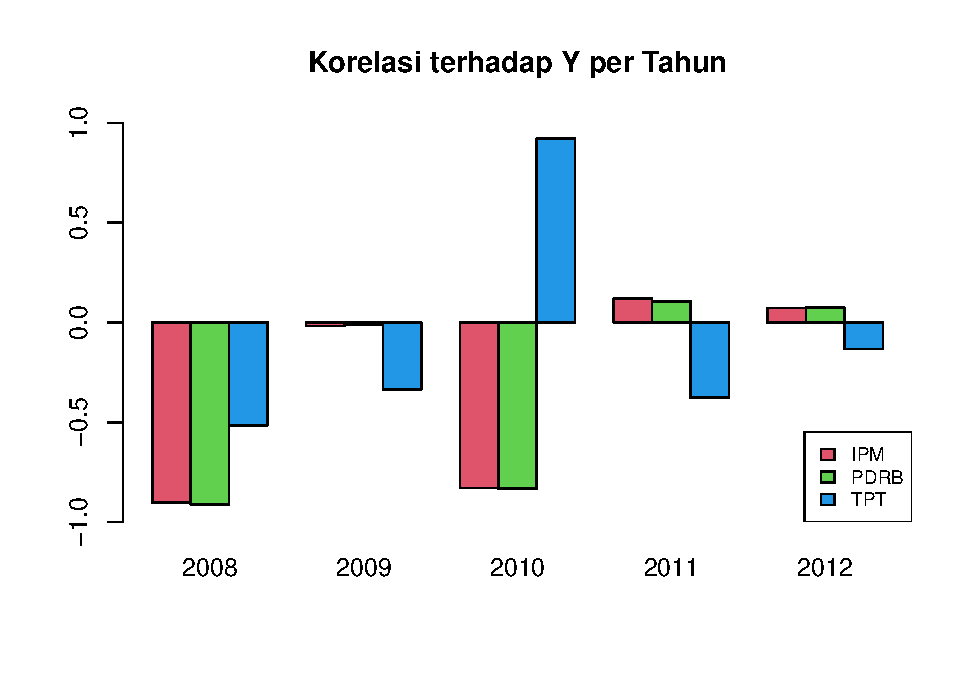
\includegraphics{modul_files/figure-latex/unnamed-chunk-96-1.pdf}

\begin{Shaded}
\begin{Highlighting}[]
\NormalTok{korelasipertahun}
\end{Highlighting}
\end{Shaded}

\begin{verbatim}
##            2008        2009       2010       2011        2012
## IPM  -0.9035923 -0.01758226 -0.8295863  0.1198465  0.07306023
## PDRB -0.9110926 -0.01161981 -0.8315061  0.1050094  0.07401256
## TPT  -0.5155555 -0.33560415  0.9220472 -0.3772710 -0.13234028
\end{verbatim}

\hypertarget{identifikasi-keragaman-antar-individu-dan-antar-waktu}{%
\section{Identifikasi Keragaman Antar Individu dan Antar Waktu}\label{identifikasi-keragaman-antar-individu-dan-antar-waktu}}

\begin{Shaded}
\begin{Highlighting}[]
\FunctionTok{boxplot}\NormalTok{(Kemiskinan}\SpecialCharTok{\textasciitilde{}}\NormalTok{Tahun, }\AttributeTok{data=}\NormalTok{data)}
\end{Highlighting}
\end{Shaded}

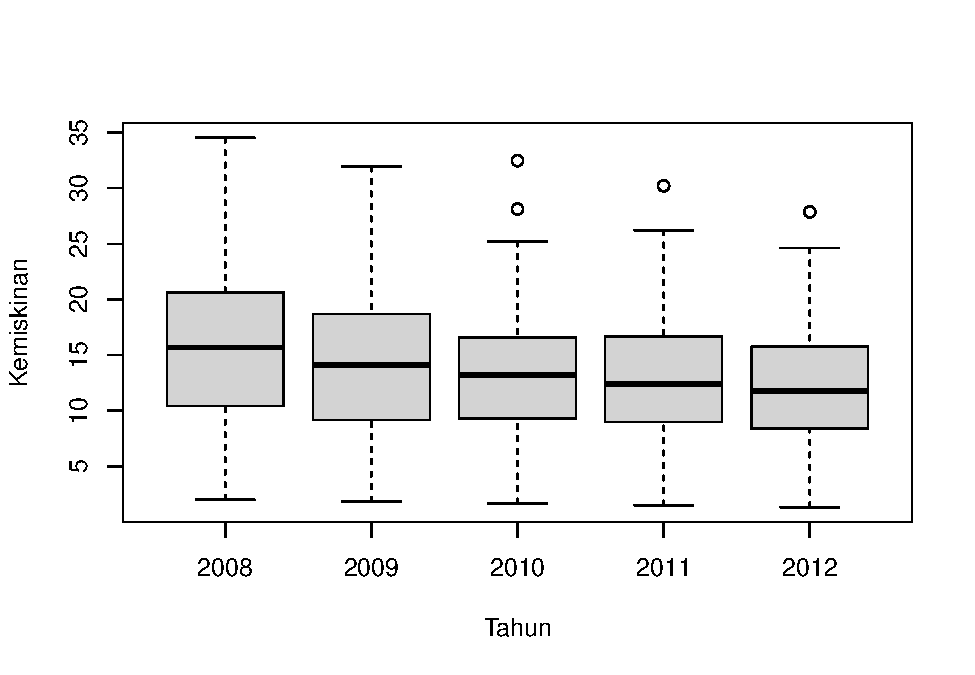
\includegraphics{modul_files/figure-latex/unnamed-chunk-98-1.pdf}

\begin{Shaded}
\begin{Highlighting}[]
\FunctionTok{boxplot}\NormalTok{(Kemiskinan}\SpecialCharTok{\textasciitilde{}}\NormalTok{KabKot, }\AttributeTok{data=}\NormalTok{data)}
\end{Highlighting}
\end{Shaded}

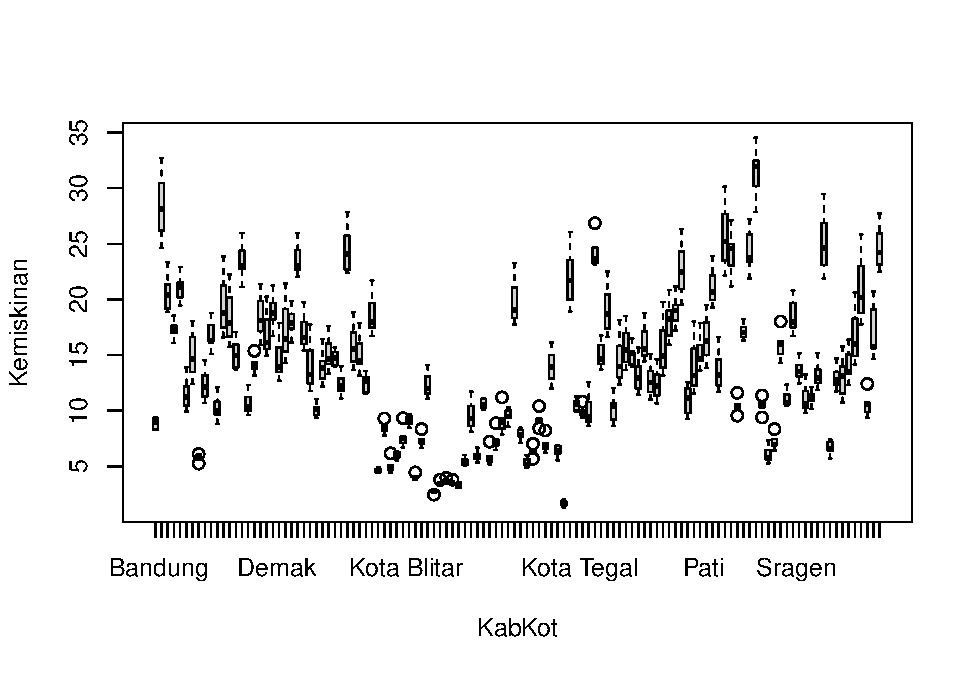
\includegraphics{modul_files/figure-latex/unnamed-chunk-99-1.pdf}

\hypertarget{pemodelan-data-panel}{%
\section{Pemodelan Data Panel}\label{pemodelan-data-panel}}

\hypertarget{model-gabungan}{%
\subsection{Model Gabungan}\label{model-gabungan}}

\begin{Shaded}
\begin{Highlighting}[]
\NormalTok{a}\OtherTok{\textless{}{-}}\FunctionTok{scale}\NormalTok{(data[,}\DecValTok{5}\SpecialCharTok{:}\DecValTok{8}\NormalTok{]) }
\NormalTok{data1}\OtherTok{\textless{}{-}}\FunctionTok{cbind}\NormalTok{(data[,}\FunctionTok{c}\NormalTok{(}\DecValTok{3}\NormalTok{,}\DecValTok{4}\NormalTok{)],a)}
\FunctionTok{head}\NormalTok{(data1)}
\end{Highlighting}
\end{Shaded}

\begin{verbatim}
##                  KabKot Tahun  Kemiskinan        IPM       PDRB       TPT
## 1           Kep. Seribu  2008 -0.01086532 -0.5558484 -0.5182081 1.0499174
## 2           Kep. Seribu  2009 -0.15332169 -0.4615811 -0.5174904 1.0239017
## 3           Kep. Seribu  2010 -0.09792199 -0.3777880 -0.5036157 0.5868385
## 4           Kep. Seribu  2011 -0.33218358 -0.2887578 -0.4729957 0.9744719
## 5           Kep. Seribu  2012 -0.31793795 -0.2128203 -0.4660583 1.6482777
## 6  Kota Jakarta Selatan  2008 -1.61745665  1.7641735  3.0389792 1.1253628
\end{verbatim}

\begin{Shaded}
\begin{Highlighting}[]
\FunctionTok{library}\NormalTok{(plm)}
\end{Highlighting}
\end{Shaded}

\begin{verbatim}
## 
## Attaching package: 'plm'
\end{verbatim}

\begin{verbatim}
## The following objects are masked from 'package:dplyr':
## 
##     between, lag, lead
\end{verbatim}

\begin{Shaded}
\begin{Highlighting}[]
\NormalTok{model.pool}\OtherTok{\textless{}{-}}\FunctionTok{plm}\NormalTok{(Kemiskinan}\SpecialCharTok{\textasciitilde{}}\NormalTok{IPM}\SpecialCharTok{+}\NormalTok{PDRB}\SpecialCharTok{+}\NormalTok{TPT, }\AttributeTok{data=}\NormalTok{data1, }\AttributeTok{model=}\StringTok{"pooling"}\NormalTok{)}
\FunctionTok{summary}\NormalTok{(model.pool)}
\end{Highlighting}
\end{Shaded}

\begin{verbatim}
## Pooling Model
## 
## Call:
## plm(formula = Kemiskinan ~ IPM + PDRB + TPT, data = data1, model = "pooling")
## 
## Balanced Panel: n = 118, T = 5, N = 590
## 
## Residuals:
##      Min.   1st Qu.    Median   3rd Qu.      Max. 
## -1.541302 -0.465061 -0.078632  0.375658  2.393066 
## 
## Coefficients:
##                Estimate  Std. Error  t-value  Pr(>|t|)    
## (Intercept)  6.9268e-16  2.7939e-02   0.0000         1    
## IPM         -5.2289e-01  3.1199e-02 -16.7600 < 2.2e-16 ***
## PDRB        -1.4241e-01  3.0670e-02  -4.6431 4.239e-06 ***
## TPT         -2.8226e-01  2.9722e-02  -9.4965 < 2.2e-16 ***
## ---
## Signif. codes:  0 '***' 0.001 '**' 0.01 '*' 0.05 '.' 0.1 ' ' 1
## 
## Total Sum of Squares:    589
## Residual Sum of Squares: 269.87
## R-Squared:      0.54181
## Adj. R-Squared: 0.53947
## F-statistic: 230.985 on 3 and 586 DF, p-value: < 2.22e-16
\end{verbatim}

Model di atas adalah model gabungan, atau sama dengan model OLS (\emph{ordinary least squares}). Selanjutnya, kita perlu mengidentifikasi apakah terdapat pengaruh individu atau waktu, atau keduanya, serta yang manakah di antara model gabungan, tetap , atau acak yang paling sesuai untuk digunakan.

\begin{Shaded}
\begin{Highlighting}[]
\FunctionTok{plmtest}\NormalTok{(model.pool,}\AttributeTok{data=}\NormalTok{data1,}\AttributeTok{type=}\StringTok{"bp"}\NormalTok{,}\AttributeTok{effect =} \StringTok{"time"}\NormalTok{)}
\end{Highlighting}
\end{Shaded}

\begin{verbatim}
## 
##  Lagrange Multiplier Test - time effects (Breusch-Pagan) for balanced
##  panels
## 
## data:  Kemiskinan ~ IPM + PDRB + TPT
## chisq = 89.555, df = 1, p-value < 2.2e-16
## alternative hypothesis: significant effects
\end{verbatim}

\begin{Shaded}
\begin{Highlighting}[]
\FunctionTok{plmtest}\NormalTok{(model.pool,}\AttributeTok{data=}\NormalTok{data1,}\AttributeTok{type=}\StringTok{"bp"}\NormalTok{,}\AttributeTok{effect =} \StringTok{"individual"}\NormalTok{)}
\end{Highlighting}
\end{Shaded}

\begin{verbatim}
## 
##  Lagrange Multiplier Test - (Breusch-Pagan) for balanced panels
## 
## data:  Kemiskinan ~ IPM + PDRB + TPT
## chisq = 893.81, df = 1, p-value < 2.2e-16
## alternative hypothesis: significant effects
\end{verbatim}

\begin{Shaded}
\begin{Highlighting}[]
\CommentTok{\#install.packages("plm")}
\FunctionTok{library}\NormalTok{(plm)}

\FunctionTok{plmtest}\NormalTok{(model.pool,}\AttributeTok{type=}\StringTok{"bp"}\NormalTok{,}\AttributeTok{effect =} \StringTok{"twoways"}\NormalTok{)}
\end{Highlighting}
\end{Shaded}

\begin{verbatim}
## 
##  Lagrange Multiplier Test - two-ways effects (Breusch-Pagan) for
##  balanced panels
## 
## data:  Kemiskinan ~ IPM + PDRB + TPT
## chisq = 983.37, df = 2, p-value < 2.2e-16
## alternative hypothesis: significant effects
\end{verbatim}

Dari hasil di atas, dapat disimpulkan bahwa terdapat pengaruh signifikan yang diakibatkan oleh waktu dan individu.

\hypertarget{uji-chow}{%
\subsection{Uji Chow}\label{uji-chow}}

Untuk mengidentifikasi salah satu di antara model gabungan dan model tetap yang lebih sesuai untuk digunakan, terlebih dulu dibangun model dengan pengaruh tetap. Terdapat empat kemungkinan model yang dapat diidentifikasi melalui uji Chow, yaitu:

\begin{enumerate}
\def\labelenumi{(\arabic{enumi})}
\item
  jika kita menolak \(H_0\) pada pengujian pengaruh spesifik individu dan waktu, maka model yang sesuai adalah model pengaruh tetap komponen sisaan dua arah
\item
  jika kita menolak \(H_0\) pada pengujian pengaruh spesifik individu, maka model yang sesuai adalah model pengaruh tetap individu
\item
  jika kita menolak \(H_0\) pada pengujian pengaruh spesifik waktu, maka model yang sesuai adalah model pengaruh tetap waktu
\item
  jika kita gagal menolak \(H_0\) pada pengujian pengaruh spesifik individu dan waktu, maka model yang sesuai adalah model gabungan.
\end{enumerate}

Pada ilustrasi ini, sebelumnya telah ditunjukkan bahwa terdapat pengaruh individu dan pengaruh waktu terhadap kemiskinan, sehingga pada tahap ini akan diuji model dengan komponen sisaan dua arah.

\begin{Shaded}
\begin{Highlighting}[]
\NormalTok{model.fixed}\OtherTok{\textless{}{-}}\FunctionTok{plm}\NormalTok{(Kemiskinan}\SpecialCharTok{\textasciitilde{}}\NormalTok{IPM}\SpecialCharTok{+}\NormalTok{PDRB}\SpecialCharTok{+}\NormalTok{TPT, }\AttributeTok{data=}\NormalTok{data1, }\AttributeTok{model=}\StringTok{"within"}\NormalTok{, }\AttributeTok{effect=}\StringTok{"twoways"}\NormalTok{)}
\FunctionTok{summary}\NormalTok{(model.fixed)}
\end{Highlighting}
\end{Shaded}

\begin{verbatim}
## Twoways effects Within Model
## 
## Call:
## plm(formula = Kemiskinan ~ IPM + PDRB + TPT, data = data1, effect = "twoways", 
##     model = "within")
## 
## Balanced Panel: n = 118, T = 5, N = 590
## 
## Residuals:
##      Min.   1st Qu.    Median   3rd Qu.      Max. 
## -0.398939 -0.069804  0.001862  0.066238  0.361103 
## 
## Coefficients:
##       Estimate Std. Error  t-value  Pr(>|t|)    
## IPM  -1.139669   0.100627 -11.3257 < 2.2e-16 ***
## PDRB  0.137278   0.029365   4.6749 3.859e-06 ***
## TPT  -0.058057   0.014710  -3.9469 9.142e-05 ***
## ---
## Signif. codes:  0 '***' 0.001 '**' 0.01 '*' 0.05 '.' 0.1 ' ' 1
## 
## Total Sum of Squares:    10.232
## Residual Sum of Squares: 7.0096
## R-Squared:      0.31495
## Adj. R-Squared: 0.13227
## F-statistic: 71.2597 on 3 and 465 DF, p-value: < 2.22e-16
\end{verbatim}

Setelah menyusun model dengan pengaruh tetap, selanjutnya kita dapat menggunakan uji Chow untuk mengidentifikasi kesesuaian model antara model gabungan atau model dengan pengaruh tetap.

\begin{Shaded}
\begin{Highlighting}[]
\FunctionTok{pFtest}\NormalTok{(model.fixed, model.pool)}
\end{Highlighting}
\end{Shaded}

\begin{verbatim}
## 
##  F test for twoways effects
## 
## data:  Kemiskinan ~ IPM + PDRB + TPT
## F = 144.11, df1 = 121, df2 = 465, p-value < 2.2e-16
## alternative hypothesis: significant effects
\end{verbatim}

Berdasarkan uji Chow pada output di atas, p-value\(<\alpha=0.05\), sehingga dapat disimpulkan bahwa model yang sesuai adalah model pengaruh tetap komponen sisaan dua arah. Selanjutnya, kita masih harus mengidentifikasi lebih lanjut apakah model pengaruh acak lebih sesuai untuk digunakan dibandingkan dengan model pengaruh tetap.

\hypertarget{uji-hausman}{%
\subsection{Uji Hausman}\label{uji-hausman}}

Pada tahap ini kita akan mengidentifikasi lebih lanjut mengenai kesuaian model antara model dengan pengaruh tetap atau pengaruh acak.

\begin{Shaded}
\begin{Highlighting}[]
\NormalTok{model.random}\OtherTok{\textless{}{-}}\FunctionTok{plm}\NormalTok{(Kemiskinan}\SpecialCharTok{\textasciitilde{}}\NormalTok{IPM}\SpecialCharTok{+}\NormalTok{PDRB}\SpecialCharTok{+}\NormalTok{TPT, }\AttributeTok{data=}\NormalTok{data1, }\AttributeTok{model=}\StringTok{"random"}\NormalTok{, }\AttributeTok{effect=}\StringTok{"twoways"}\NormalTok{)}
\FunctionTok{summary}\NormalTok{(model.random)}
\end{Highlighting}
\end{Shaded}

\begin{verbatim}
## Twoways effects Random Effect Model 
##    (Swamy-Arora's transformation)
## 
## Call:
## plm(formula = Kemiskinan ~ IPM + PDRB + TPT, data = data1, effect = "twoways", 
##     model = "random")
## 
## Balanced Panel: n = 118, T = 5, N = 590
## 
## Effects:
##                     var   std.dev share
## idiosyncratic 0.0150743 0.1227776 0.035
## individual    0.4111332 0.6411967 0.964
## time          0.0001843 0.0135741 0.000
## theta: 0.9147 (id) 0.3601 (time) 0.3597 (total)
## 
## Residuals:
##      Min.   1st Qu.    Median   3rd Qu.      Max. 
## -0.454852 -0.083503 -0.010059  0.071157  0.533129 
## 
## Coefficients:
##                Estimate  Std. Error  z-value  Pr(>|z|)    
## (Intercept)  1.4693e-15  6.5106e-02   0.0000  1.000000    
## IPM         -1.0194e+00  3.9214e-02 -25.9955 < 2.2e-16 ***
## PDRB         9.0152e-02  2.8350e-02   3.1800  0.001473 ** 
## TPT         -4.1548e-02  1.4364e-02  -2.8925  0.003822 ** 
## ---
## Signif. codes:  0 '***' 0.001 '**' 0.01 '*' 0.05 '.' 0.1 ' ' 1
## 
## Total Sum of Squares:    22.996
## Residual Sum of Squares: 10.558
## R-Squared:      0.5409
## Adj. R-Squared: 0.53855
## Chisq: 690.408 on 3 DF, p-value: < 2.22e-16
\end{verbatim}

Hipotesis yang diuji pada uji Hausman adalah:

\begin{quote}
\(H_0: E(u_{it}|x_{k, it})=0\) (model pengaruh acak)
\end{quote}

\begin{quote}
\(H_1: E(u_{it}|x_{k, it}) \ne 0\) (model pengaruh tetap)
\end{quote}

\begin{Shaded}
\begin{Highlighting}[]
\FunctionTok{phtest}\NormalTok{(model.fixed, model.random)}
\end{Highlighting}
\end{Shaded}

\begin{verbatim}
## 
##  Hausman Test
## 
## data:  Kemiskinan ~ IPM + PDRB + TPT
## chisq = 57.774, df = 3, p-value = 1.756e-12
## alternative hypothesis: one model is inconsistent
\end{verbatim}

Terlihat pada output bahwa kita dapat menolak hipotesis nol pada taraf nyata 0.05, artinya model yang lebih tepat digunakan adalah model dengan pengaruh tetap.

\begin{Shaded}
\begin{Highlighting}[]
\FunctionTok{summary}\NormalTok{(model.fixed)}
\end{Highlighting}
\end{Shaded}

\begin{verbatim}
## Twoways effects Within Model
## 
## Call:
## plm(formula = Kemiskinan ~ IPM + PDRB + TPT, data = data1, effect = "twoways", 
##     model = "within")
## 
## Balanced Panel: n = 118, T = 5, N = 590
## 
## Residuals:
##      Min.   1st Qu.    Median   3rd Qu.      Max. 
## -0.398939 -0.069804  0.001862  0.066238  0.361103 
## 
## Coefficients:
##       Estimate Std. Error  t-value  Pr(>|t|)    
## IPM  -1.139669   0.100627 -11.3257 < 2.2e-16 ***
## PDRB  0.137278   0.029365   4.6749 3.859e-06 ***
## TPT  -0.058057   0.014710  -3.9469 9.142e-05 ***
## ---
## Signif. codes:  0 '***' 0.001 '**' 0.01 '*' 0.05 '.' 0.1 ' ' 1
## 
## Total Sum of Squares:    10.232
## Residual Sum of Squares: 7.0096
## R-Squared:      0.31495
## Adj. R-Squared: 0.13227
## F-statistic: 71.2597 on 3 and 465 DF, p-value: < 2.22e-16
\end{verbatim}

Model dapat dituliskan sebagai berikut:

\[y_{it}=-1.139669x_{1it}+0.137278x_{2it}-0.058057x_{3it}+\hat{\mu}_i+\varepsilon_{it}\]

\hypertarget{pemodelan-data-panel-spasial}{%
\section{Pemodelan Data Panel Spasial}\label{pemodelan-data-panel-spasial}}

Peta persebaran jumlah penduduk miskin di kabupaten/kota di pulau Jawa pada tahun 2012 terlihat pada gambar berikut.

\begin{Shaded}
\begin{Highlighting}[]
\FunctionTok{library}\NormalTok{(rgdal)}
\FunctionTok{library}\NormalTok{(spdep)}
\FunctionTok{library}\NormalTok{(raster)}
\FunctionTok{library}\NormalTok{(sp)}
\FunctionTok{library}\NormalTok{(spatialreg)}

\NormalTok{petajawa}\OtherTok{\textless{}{-}}\FunctionTok{readOGR}\NormalTok{(}\AttributeTok{dsn=}\StringTok{\textquotesingle{}Jawamap\textquotesingle{}}\NormalTok{,}\AttributeTok{layer=}\StringTok{\textquotesingle{}jawa\textquotesingle{}}\NormalTok{)}
\end{Highlighting}
\end{Shaded}

\begin{verbatim}
## OGR data source with driver: ESRI Shapefile 
## Source: "D:\Jobs\Pelatihan Spasial STIS\New folder\Pelatihan-Spasial\Jawamap", layer: "jawa"
## with 119 features
## It has 5 fields
\end{verbatim}

\begin{Shaded}
\begin{Highlighting}[]
\NormalTok{petajawa}\SpecialCharTok{@}\NormalTok{data[}\DecValTok{24}\NormalTok{,] }\CommentTok{\#dihilangkan dari peta karena tidak ada dalam data pengamatan}
\end{Highlighting}
\end{Shaded}

\begin{verbatim}
##    PROVNO KABKOTNO   PROVINSI      KABKOT ID2013
## 23     32       18 JAWA BARAT PANGANDARAN   3218
\end{verbatim}

\begin{Shaded}
\begin{Highlighting}[]
\NormalTok{petajawa}\OtherTok{\textless{}{-}}\NormalTok{petajawa[}\SpecialCharTok{{-}}\DecValTok{24}\NormalTok{,]}


\NormalTok{data2012}\OtherTok{\textless{}{-}}\FunctionTok{subset}\NormalTok{(data, data}\SpecialCharTok{$}\NormalTok{Tahun}\SpecialCharTok{==}\DecValTok{2012}\NormalTok{)}

\NormalTok{petajawa}\SpecialCharTok{$}\NormalTok{Kemiskinan}\OtherTok{\textless{}{-}}\NormalTok{data2012}\SpecialCharTok{$}\NormalTok{Kemiskinan}
\FunctionTok{spplot}\NormalTok{(petajawa, }\StringTok{"Kemiskinan"}\NormalTok{, }\AttributeTok{main=}\StringTok{"Persentase Penduduk Miskin 2012"}\NormalTok{)}
\end{Highlighting}
\end{Shaded}

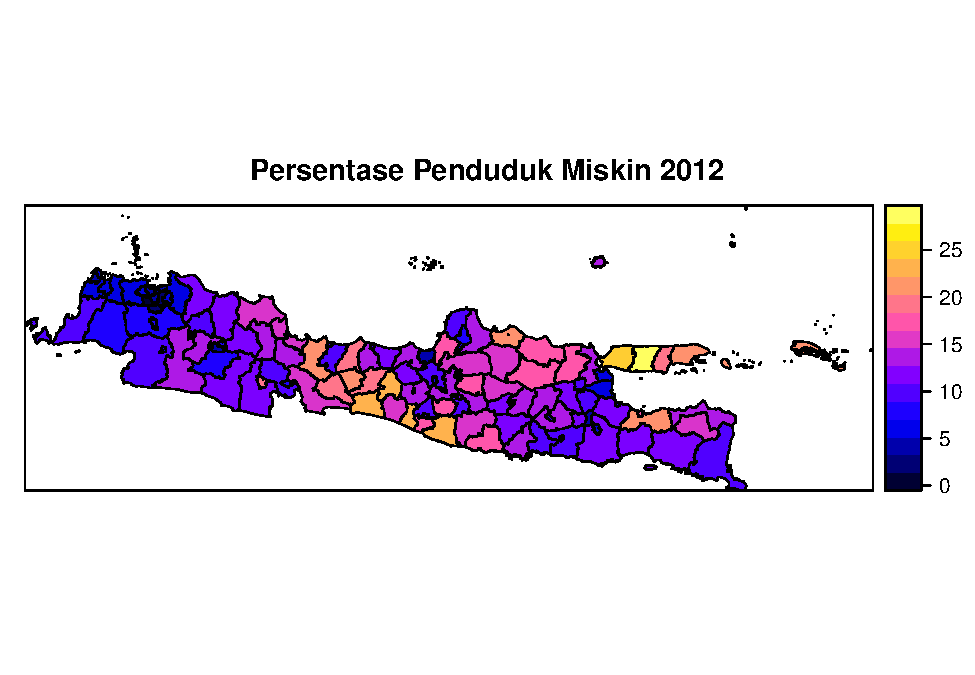
\includegraphics{modul_files/figure-latex/unnamed-chunk-110-1.pdf}

\hypertarget{uji-ketergantungan-spasial-pada-data-panel}{%
\subsection{Uji Ketergantungan Spasial pada Data Panel}\label{uji-ketergantungan-spasial-pada-data-panel}}

Seperti yang telah dijelaskan pada bagian awal modul ini, kita dapat menggunakan uji \emph{cross-sectional dependency} (CD) Pesaran untuk mengidentifikasi ketergantungan spasial pada data panel.

\begin{Shaded}
\begin{Highlighting}[]
\FunctionTok{library}\NormalTok{(splm)}
\end{Highlighting}
\end{Shaded}

\begin{verbatim}
## Warning: package 'splm' was built under R version 4.0.4
\end{verbatim}

\begin{Shaded}
\begin{Highlighting}[]
\NormalTok{w}\OtherTok{\textless{}{-}}\FunctionTok{as.matrix}\NormalTok{(}\DecValTok{1}\SpecialCharTok{/}\FunctionTok{dist}\NormalTok{(}\FunctionTok{coordinates}\NormalTok{(petajawa)))}
\NormalTok{ww}\OtherTok{\textless{}{-}}\NormalTok{w}
\ControlFlowTok{for}\NormalTok{(i }\ControlFlowTok{in} \DecValTok{1}\SpecialCharTok{:}\DecValTok{118}\NormalTok{)}
\NormalTok{\{}
\NormalTok{ww[i,]}\OtherTok{\textless{}{-}}\NormalTok{ww[i,]}\SpecialCharTok{/}\FunctionTok{apply}\NormalTok{(w,}\DecValTok{1}\NormalTok{,sum)[i]}
\NormalTok{\}}
\FunctionTok{rowSums}\NormalTok{(ww)}
\end{Highlighting}
\end{Shaded}

\begin{verbatim}
##   0   1   2   3   4   5   6   7   8   9  10  11  12  13  14  15  16  17  18  19 
##   1   1   1   1   1   1   1   1   1   1   1   1   1   1   1   1   1   1   1   1 
##  20  21  22  24  25  26  27  28  29  30  31  32  33  34  35  36  37  38  39  40 
##   1   1   1   1   1   1   1   1   1   1   1   1   1   1   1   1   1   1   1   1 
##  41  42  43  44  45  46  47  48  49  50  51  52  53  54  55  56  57  58  59  60 
##   1   1   1   1   1   1   1   1   1   1   1   1   1   1   1   1   1   1   1   1 
##  61  62  63  64  65  66  67  68  69  70  71  72  73  74  75  76  77  78  79  80 
##   1   1   1   1   1   1   1   1   1   1   1   1   1   1   1   1   1   1   1   1 
##  81  82  83  84  85  86  87  88  89  90  91  92  93  94  95  96  97  98  99 100 
##   1   1   1   1   1   1   1   1   1   1   1   1   1   1   1   1   1   1   1   1 
## 101 102 103 104 105 106 107 108 109 110 111 112 113 114 115 116 117 118 
##   1   1   1   1   1   1   1   1   1   1   1   1   1   1   1   1   1   1
\end{verbatim}

\begin{Shaded}
\begin{Highlighting}[]
\FunctionTok{rwtest}\NormalTok{(model.fixed, }\AttributeTok{w=}\NormalTok{ww)}
\end{Highlighting}
\end{Shaded}

\begin{verbatim}
## 
##  Randomized W test for spatial correlation of order 1
## 
## data:  formula
## p-value < 2.2e-16
## alternative hypothesis: twosided
\end{verbatim}

Terlihat pada output di atas bahwa p-value \(<\alpha=0.05\) maka kita dapat menyimpulkan bahwa hipotesis nol ditolak, artinya pada data panel kemiskinan ini terdapat ketergantungan spasial pada peubah responnya. Hal ini mengindikasikan bahwa kemiskinan di suatu kab/kota, selain dipengaruhi oleh peubah penjelas yang dimilikinya, juga dipengaruhi oleh kemiskinan di kab/kota lain.

\hypertarget{uji-spesifikasi-model}{%
\subsection{Uji Spesifikasi Model}\label{uji-spesifikasi-model}}

Menurut Salima \emph{et. al,} spesifikasi model pada pemodelan data panel spasial adalah sebagai berikut.

\hypertarget{standard-model-model-dengan-pengaruh-spesifik-individu}{%
\subsection{Standard model: model dengan pengaruh spesifik individu}\label{standard-model-model-dengan-pengaruh-spesifik-individu}}

\(y_{it}=x_{it}\beta + z_i\alpha + \varepsilon_{it}\)

dimana \(z_i\alpha\) merupakan pengaruh spesifik individu.

\textbf{Model gabungan}

\(y_{it}=x_{it}\beta + \alpha + \varepsilon_{it}\)

Model ini tidak memodelkan heterogenitas individu, dan pada kasus ini penduga \(\beta\) dan \(\alpha\) diperoleh dengan Ordinary Least Squares (OLS).

\textbf{Model Pengaruh Tetap}

\(y_{it}=x_{it}\beta + \alpha_i + \varepsilon_{it}\)

\textbf{Model Pengaruh Acak}

\(y_{it}=x_{it}\beta + \alpha + u_{it}\)
\(u_{it}=\alpha_i + \varepsilon_{it}\)

Model ini biasanya diduga dengan Generalized Least Squares (GLS).

\hypertarget{efek-spasial-pada-model-data-panel}{%
\subsection{Efek Spasial pada Model Data Panel}\label{efek-spasial-pada-model-data-panel}}

\textbf{Efek spasial pada model gabungan}

\(y_{it}=\rho\sum_{i \ne j} w_{ij} y_{jt} + x_{it}\beta + \sum_{i \ne j} w_{ij} x_{jt} \theta + \alpha + u_{it}\)

\(u_{it}=\lambda \sum_{i \ne j} w_{ij} u_{jt} + \varepsilon_{it}\)

\textbf{Efek spasial pada model pengaruh tetap}

\begin{enumerate}
\def\labelenumi{(\arabic{enumi})}
\item
  Spatial autoregressive model (SAR)

  \(y_{it}=\rho\sum_{i \ne j} w_{ij} y_{jt} + x_{it}\beta + \alpha_i + u_{it}\)
\item
  Spatial error model (SEM)

  \(y_{it}= x_{it}\beta + \alpha_i + u_{it}\)

  \(u_{it}=\lambda \sum_{i \ne j} w_{ij} u_{jt} + \varepsilon_{it}\)
\item
  Durbin spatial model (DSM)

  \(y_{it}=x_{it}\beta + \sum_{i \ne j} w_{ij} x_{jt} \theta + \alpha_i + u_{it}\)
\item
  Durbin spatial error model (SDEM)

  \(y_{it}= x_{it}\beta + \sum_{i \ne j} w_{ij} x_{jt} \theta + \alpha_i + u_{it}\)

  \(u_{it}=\lambda \sum_{i \ne j} w_{ij} u_{jt} + \varepsilon_{it}\)
\item
  Spatial autoregressive lag and error model (SARAR)

  \(y_{it}=\rho\sum_{i \ne j} w_{ij} y_{jt} + x_{it}\beta + \alpha_i + u_{it}\)

  \(u_{it}=\lambda \sum_{i \ne j} m_{ij} u_{jt} + \varepsilon_{it}\)

  dimana \(w_{ij}\) dan \(m_{ij}\) merupakan pembobot spasial.
\end{enumerate}

\textbf{Spatial Error Model-Random Effect}

\(y_{it}=\rho\sum_{i \ne j} w_{ij} y_{jt} + x_{it}\beta + \alpha + u_{it}\)

\(u_{it}=\lambda \sum_{i \ne j} w_{ij} u_{jt} + \nu_{it}\)

\hypertarget{hausmans-robust-test-of-spatial-autocorrelation}{%
\subsubsection{Hausman's robust test of spatial autocorrelation}\label{hausmans-robust-test-of-spatial-autocorrelation}}

Uji ini dilakukan untuk mengidentifikasi kesesuaian model dengan pengaruh tetap atau acak. Hipotesis nol yang diuji adalah: \(H_0: E[\alpha|X]=0\). Jika hipotesis ini ditolak, artinya model yang lebih sesuai adalah model dengan pengaruh tetap.

\begin{Shaded}
\begin{Highlighting}[]
\FunctionTok{library}\NormalTok{(splm)}
\FunctionTok{print}\NormalTok{(panelhausman}\OtherTok{\textless{}{-}}\FunctionTok{phtest}\NormalTok{(Kemiskinan}\SpecialCharTok{\textasciitilde{}}\NormalTok{IPM}\SpecialCharTok{+}\NormalTok{PDRB}\SpecialCharTok{+}\NormalTok{TPT, }\AttributeTok{data=}\NormalTok{data1))}
\end{Highlighting}
\end{Shaded}

\begin{verbatim}
## 
##  Hausman Test
## 
## data:  Kemiskinan ~ IPM + PDRB + TPT
## chisq = 226.68, df = 3, p-value < 2.2e-16
## alternative hypothesis: one model is inconsistent
\end{verbatim}

\begin{Shaded}
\begin{Highlighting}[]
\FunctionTok{print}\NormalTok{(spat.hausman.SEM}\OtherTok{\textless{}{-}}\FunctionTok{sphtest}\NormalTok{(Kemiskinan}\SpecialCharTok{\textasciitilde{}}\NormalTok{IPM}\SpecialCharTok{+}\NormalTok{PDRB}\SpecialCharTok{+}\NormalTok{TPT, }\AttributeTok{data=}\NormalTok{data1, }\AttributeTok{listw=}\FunctionTok{mat2listw}\NormalTok{(ww),}\AttributeTok{spatial.model=}\StringTok{"error"}\NormalTok{))}
\end{Highlighting}
\end{Shaded}

\begin{verbatim}
## 
##  Hausman test for spatial models
## 
## data:  x
## chisq = 39.506, df = 3, p-value = 1.356e-08
## alternative hypothesis: one model is inconsistent
\end{verbatim}

\begin{Shaded}
\begin{Highlighting}[]
\FunctionTok{print}\NormalTok{(spat.hausman.SAR}\OtherTok{\textless{}{-}}\FunctionTok{sphtest}\NormalTok{(Kemiskinan}\SpecialCharTok{\textasciitilde{}}\NormalTok{IPM}\SpecialCharTok{+}\NormalTok{PDRB}\SpecialCharTok{+}\NormalTok{TPT, }\AttributeTok{data=}\NormalTok{data1, }\AttributeTok{listw=}\FunctionTok{mat2listw}\NormalTok{(ww),}\AttributeTok{spatial.model=}\StringTok{"lag"}\NormalTok{))}
\end{Highlighting}
\end{Shaded}

\begin{verbatim}
## 
##  Hausman test for spatial models
## 
## data:  x
## chisq = 36.181, df = 3, p-value = 6.857e-08
## alternative hypothesis: one model is inconsistent
\end{verbatim}

Terlihat pada output di atas, maka model yang lebih sesuai digunakan adalah model dengan pengaruh tetap.

\hypertarget{uji-spesifikasi-untuk-pengaruh-spasial}{%
\subsubsection{Uji Spesifikasi untuk Pengaruh Spasial}\label{uji-spesifikasi-untuk-pengaruh-spasial}}

Fungsi \texttt{bsktest} dapat menghitung uji gabungan, marginal, ataupun conditional untuk pengaruh acak dan korelasi galat spasial. Hipotesis yang diuji adalah sebagai berikut. (Milo dan Piras, 2012)
\includegraphics{D:/Research (eksternal dept)/pelatihan spasial (adj)/modul dept}/pelatihan spasial (adj)/Modul/hipotesis-lm-splm.PNG)

Untuk model tetap, uji Lagrange dapat dilakukan untuk mengidentifikasi spesifikasi pengaruh spasial pada model.

\begin{Shaded}
\begin{Highlighting}[]
\CommentTok{\# Uji 1}
\FunctionTok{slmtest}\NormalTok{(Kemiskinan}\SpecialCharTok{\textasciitilde{}}\NormalTok{IPM}\SpecialCharTok{+}\NormalTok{PDRB}\SpecialCharTok{+}\NormalTok{TPT, }\AttributeTok{data=}\NormalTok{data1, }\AttributeTok{listw=}\FunctionTok{mat2listw}\NormalTok{(ww),}\AttributeTok{test=}\StringTok{"lml"}\NormalTok{, }\AttributeTok{model=}\StringTok{"within"}\NormalTok{)}
\end{Highlighting}
\end{Shaded}

\begin{verbatim}
## 
##  LM test for spatial lag dependence
## 
## data:  formula (within transformation)
## LM = 86.153, df = 1, p-value < 2.2e-16
## alternative hypothesis: spatial lag dependence
\end{verbatim}

\begin{Shaded}
\begin{Highlighting}[]
\CommentTok{\# Uji 2}
\FunctionTok{slmtest}\NormalTok{(Kemiskinan}\SpecialCharTok{\textasciitilde{}}\NormalTok{IPM}\SpecialCharTok{+}\NormalTok{PDRB}\SpecialCharTok{+}\NormalTok{TPT, }\AttributeTok{data=}\NormalTok{data1, }\AttributeTok{listw=}\FunctionTok{mat2listw}\NormalTok{(ww),}\AttributeTok{test=}\StringTok{"lme"}\NormalTok{, }\AttributeTok{model=}\StringTok{"within"}\NormalTok{)}
\end{Highlighting}
\end{Shaded}

\begin{verbatim}
## 
##  LM test for spatial error dependence
## 
## data:  formula (within transformation)
## LM = 239.59, df = 1, p-value < 2.2e-16
## alternative hypothesis: spatial error dependence
\end{verbatim}

Uji robust dapat dilakukan untuk membantu menentukan spesifikasi model apabila uji sebelumnya, kedua uji untuk model SAR dan SEM sama-sama siginifikan.

\begin{Shaded}
\begin{Highlighting}[]
\CommentTok{\# Uji 3}

\FunctionTok{slmtest}\NormalTok{(Kemiskinan}\SpecialCharTok{\textasciitilde{}}\NormalTok{IPM}\SpecialCharTok{+}\NormalTok{PDRB}\SpecialCharTok{+}\NormalTok{TPT, }\AttributeTok{data=}\NormalTok{data1, }\AttributeTok{listw=}\FunctionTok{mat2listw}\NormalTok{(ww),}\AttributeTok{test=}\StringTok{"rlml"}\NormalTok{, }\AttributeTok{model=}\StringTok{"within"}\NormalTok{)}
\end{Highlighting}
\end{Shaded}

\begin{verbatim}
## 
##  Locally robust LM test for spatial lag dependence sub spatial error
## 
## data:  formula (within transformation)
## LM = 2.3656, df = 1, p-value = 0.124
## alternative hypothesis: spatial lag dependence
\end{verbatim}

\begin{Shaded}
\begin{Highlighting}[]
\CommentTok{\# Uji 4}

\FunctionTok{slmtest}\NormalTok{(Kemiskinan}\SpecialCharTok{\textasciitilde{}}\NormalTok{IPM}\SpecialCharTok{+}\NormalTok{PDRB}\SpecialCharTok{+}\NormalTok{TPT, }\AttributeTok{data=}\NormalTok{data1, }\AttributeTok{listw=}\FunctionTok{mat2listw}\NormalTok{(ww),}\AttributeTok{test=}\StringTok{"rlme"}\NormalTok{, }\AttributeTok{model=}\StringTok{"within"}\NormalTok{)}
\end{Highlighting}
\end{Shaded}

\begin{verbatim}
## 
##  Locally robust LM test for spatial error dependence sub spatial lag
## 
## data:  formula (within transformation)
## LM = 155.8, df = 1, p-value < 2.2e-16
## alternative hypothesis: spatial error dependence
\end{verbatim}

\hypertarget{model-panel-sar}{%
\subsection{Model Panel SAR}\label{model-panel-sar}}

\begin{Shaded}
\begin{Highlighting}[]
\NormalTok{panel.sar}\OtherTok{\textless{}{-}}\FunctionTok{spml}\NormalTok{(Kemiskinan}\SpecialCharTok{\textasciitilde{}}\NormalTok{IPM}\SpecialCharTok{+}\NormalTok{PDRB}\SpecialCharTok{+}\NormalTok{TPT, }\AttributeTok{data=}\NormalTok{data1, }\AttributeTok{listw=}\FunctionTok{mat2listw}\NormalTok{(ww),}\AttributeTok{model=}\StringTok{"within"}\NormalTok{, }
                \AttributeTok{effect =} \StringTok{"twoways"}\NormalTok{, }\AttributeTok{lag=}\NormalTok{T, }\AttributeTok{spatial.error =} \StringTok{"none"}\NormalTok{)}
\FunctionTok{summary}\NormalTok{(panel.sar)}
\end{Highlighting}
\end{Shaded}

\begin{verbatim}
## Spatial panel fixed effects lag model
##  
## 
## Call:
## spml(formula = Kemiskinan ~ IPM + PDRB + TPT, data = data1, listw = mat2listw(ww), 
##     model = "within", effect = "twoways", lag = T, spatial.error = "none")
## 
## Residuals:
##       Min.    1st Qu.     Median    3rd Qu.       Max. 
## -0.3547835 -0.0672962  0.0054614  0.0652831  0.3475310 
## 
## Spatial autoregressive coefficient:
##        Estimate Std. Error t-value  Pr(>|t|)    
## lambda  0.52996    0.09744  5.4389 5.362e-08 ***
## 
## Coefficients:
##       Estimate Std. Error  t-value  Pr(>|t|)    
## IPM  -1.132105   0.086967 -13.0176 < 2.2e-16 ***
## PDRB  0.121054   0.025466   4.7535 1.999e-06 ***
## TPT  -0.047154   0.012776  -3.6909 0.0002234 ***
## ---
## Signif. codes:  0 '***' 0.001 '**' 0.01 '*' 0.05 '.' 0.1 ' ' 1
\end{verbatim}

\begin{Shaded}
\begin{Highlighting}[]
\CommentTok{\#db=t*n{-}(k+1){-}n}
\NormalTok{db}\OtherTok{\textless{}{-}}\NormalTok{(}\DecValTok{5}\SpecialCharTok{*}\DecValTok{118}\NormalTok{)}\SpecialCharTok{{-}}\NormalTok{(}\DecValTok{3}\SpecialCharTok{+}\DecValTok{1}\NormalTok{)}\SpecialCharTok{{-}}\DecValTok{118}
  
\FunctionTok{sqrt}\NormalTok{(}\FunctionTok{sum}\NormalTok{(panel.sar}\SpecialCharTok{$}\NormalTok{resid}\SpecialCharTok{\^{}}\DecValTok{2}\NormalTok{)}\SpecialCharTok{/}\NormalTok{db) }\DocumentationTok{\#\# Standard Error of Regression}
\end{Highlighting}
\end{Shaded}

\begin{verbatim}
## [1] 0.1191296
\end{verbatim}

\begin{Shaded}
\begin{Highlighting}[]
\FunctionTok{summary}\NormalTok{(panel.sar)}\SpecialCharTok{$}\NormalTok{rsqr }\DocumentationTok{\#\# Pseudo{-}R2}
\end{Highlighting}
\end{Shaded}

\begin{verbatim}
## [1] 0.9887236
\end{verbatim}

\hypertarget{model-panel-sem}{%
\subsection{Model Panel SEM}\label{model-panel-sem}}

\begin{Shaded}
\begin{Highlighting}[]
\NormalTok{panel.sem}\OtherTok{\textless{}{-}}\FunctionTok{spml}\NormalTok{(Kemiskinan}\SpecialCharTok{\textasciitilde{}}\NormalTok{IPM}\SpecialCharTok{+}\NormalTok{PDRB}\SpecialCharTok{+}\NormalTok{TPT, }\AttributeTok{data=}\NormalTok{data1, }\AttributeTok{listw=}\FunctionTok{mat2listw}\NormalTok{(ww),}\AttributeTok{model=}\StringTok{"within"}\NormalTok{, }
                \AttributeTok{effect =} \StringTok{"twoways"}\NormalTok{, }\AttributeTok{lag=}\NormalTok{F)}
\FunctionTok{summary}\NormalTok{(panel.sem)}
\end{Highlighting}
\end{Shaded}

\begin{verbatim}
## Spatial panel fixed effects error model
##  
## 
## Call:
## spml(formula = Kemiskinan ~ IPM + PDRB + TPT, data = data1, listw = mat2listw(ww), 
##     model = "within", effect = "twoways", lag = F)
## 
## Residuals:
##       Min.    1st Qu.     Median    3rd Qu.       Max. 
## -0.4023151 -0.0699875  0.0011909  0.0672228  0.3628160 
## 
## Spatial error parameter:
##     Estimate Std. Error t-value  Pr(>|t|)    
## rho  0.51726    0.10568  4.8948 9.841e-07 ***
## 
## Coefficients:
##       Estimate Std. Error  t-value  Pr(>|t|)    
## IPM  -1.121679   0.086057 -13.0341 < 2.2e-16 ***
## PDRB  0.126167   0.026015   4.8497 1.236e-06 ***
## TPT  -0.047787   0.013025  -3.6688 0.0002437 ***
## ---
## Signif. codes:  0 '***' 0.001 '**' 0.01 '*' 0.05 '.' 0.1 ' ' 1
\end{verbatim}

\begin{Shaded}
\begin{Highlighting}[]
\FunctionTok{sqrt}\NormalTok{(}\FunctionTok{sum}\NormalTok{(panel.sem}\SpecialCharTok{$}\NormalTok{resid}\SpecialCharTok{\^{}}\DecValTok{2}\NormalTok{)}\SpecialCharTok{/}\NormalTok{db) }\DocumentationTok{\#\# Standard Error of Regression}
\end{Highlighting}
\end{Shaded}

\begin{verbatim}
## [1] 0.1224889
\end{verbatim}

\begin{Shaded}
\begin{Highlighting}[]
\FunctionTok{summary}\NormalTok{(panel.sem)}\SpecialCharTok{$}\NormalTok{rsqr }\DocumentationTok{\#\# Pseudo{-}R2}
\end{Highlighting}
\end{Shaded}

\begin{verbatim}
## [1] 0.9880787
\end{verbatim}

\hypertarget{model-panel-gsm}{%
\subsection{Model Panel GSM}\label{model-panel-gsm}}

\begin{Shaded}
\begin{Highlighting}[]
\NormalTok{panel.gsm}\OtherTok{\textless{}{-}}\FunctionTok{spml}\NormalTok{(Kemiskinan}\SpecialCharTok{\textasciitilde{}}\NormalTok{IPM}\SpecialCharTok{+}\NormalTok{PDRB}\SpecialCharTok{+}\NormalTok{TPT, }\AttributeTok{data=}\NormalTok{data1, }\AttributeTok{listw=}\FunctionTok{mat2listw}\NormalTok{(ww),}\AttributeTok{model=}\StringTok{"within"}\NormalTok{, }
                \AttributeTok{effect =} \StringTok{"twoways"}\NormalTok{, }\AttributeTok{lag=}\NormalTok{T)}
\FunctionTok{summary}\NormalTok{(panel.gsm)}
\end{Highlighting}
\end{Shaded}

\begin{verbatim}
## Spatial panel fixed effects sarar model
##  
## 
## Call:
## spml(formula = Kemiskinan ~ IPM + PDRB + TPT, data = data1, listw = mat2listw(ww), 
##     model = "within", effect = "twoways", lag = T)
## 
## Residuals:
##       Min.    1st Qu.     Median    3rd Qu.       Max. 
## -0.3359218 -0.0646201  0.0040778  0.0639445  0.3500236 
## 
## Spatial error parameter:
##     Estimate Std. Error t-value Pr(>|t|)  
## rho -0.43578    0.22909 -1.9022  0.05714 .
## 
## Spatial autoregressive coefficient:
##        Estimate Std. Error t-value  Pr(>|t|)    
## lambda 0.721893   0.094678  7.6247 2.445e-14 ***
## 
## Coefficients:
##       Estimate Std. Error  t-value  Pr(>|t|)    
## IPM  -1.121340   0.086980 -12.8919 < 2.2e-16 ***
## PDRB  0.119617   0.024785   4.8262 1.391e-06 ***
## TPT  -0.047253   0.012451  -3.7951 0.0001476 ***
## ---
## Signif. codes:  0 '***' 0.001 '**' 0.01 '*' 0.05 '.' 0.1 ' ' 1
\end{verbatim}

\begin{Shaded}
\begin{Highlighting}[]
\FunctionTok{sqrt}\NormalTok{(}\FunctionTok{sum}\NormalTok{(panel.gsm}\SpecialCharTok{$}\NormalTok{resid}\SpecialCharTok{\^{}}\DecValTok{2}\NormalTok{)}\SpecialCharTok{/}\NormalTok{db) }\DocumentationTok{\#\# Standard Error of Regression}
\end{Highlighting}
\end{Shaded}

\begin{verbatim}
## [1] 0.118768
\end{verbatim}

\begin{Shaded}
\begin{Highlighting}[]
\FunctionTok{summary}\NormalTok{(panel.gsm)}\SpecialCharTok{$}\NormalTok{rsqr }\DocumentationTok{\#\# Pseudo{-}R2}
\end{Highlighting}
\end{Shaded}

\begin{verbatim}
## [1] 0.988792
\end{verbatim}

\hypertarget{menentukan-model-terbaik-1}{%
\subsection{Menentukan Model Terbaik}\label{menentukan-model-terbaik-1}}

Berikut ini adalah ringkasan dari pemodelan yang telah dilakukan pada tahap-tahap sebelumnya:

\begin{verbatim}
##            Kriteria Panel_SAR Panel_SEM PANEL_GSM
## 1  SE of Regression    0.1191    0.1225    0.1188
## 2         Pseudo-R2    0.9887    0.9881    0.9888
## 3 p-value of lambda    0.0000        NA    0.0000
## 4    p-value of rho        NA    0.0000    0.0571
\end{verbatim}

Berdasarkan output di atas, model terbaik adalah model panel SAR.

\hypertarget{interpretasi-model}{%
\subsection{Interpretasi Model}\label{interpretasi-model}}

\begin{Shaded}
\begin{Highlighting}[]
\NormalTok{lw}\OtherTok{\textless{}{-}} \FunctionTok{mat2listw}\NormalTok{(ww, }\AttributeTok{style =}\StringTok{"W"}\NormalTok{)}

\NormalTok{spdep}\SpecialCharTok{::}\FunctionTok{impacts}\NormalTok{(panel.sar, }\AttributeTok{listw=}\NormalTok{lw, }\AttributeTok{time =} \DecValTok{5}\NormalTok{)}
\end{Highlighting}
\end{Shaded}

\begin{verbatim}
## Impact measures (lag, trace):
##           Direct   Indirect      Total
## IPM  -1.14756006 -1.2609854 -2.4085455
## PDRB  0.12270607  0.1348344  0.2575405
## TPT  -0.04779766 -0.0525220 -0.1003197
\end{verbatim}

\hypertarget{sumber-pustaka-3}{%
\section{Sumber Pustaka}\label{sumber-pustaka-3}}

Agusti, R. (2015). Pemodelan data panel kemiskinan tak seimbang di pulau Jawa dnegna model spasial durbin {[}Tesis{]}. IPB.

Millo, G., \& Piras, G. (2012). splm: Spatial panel data models in R. Journal of Statistical Software, 47(1), 1-38.

Salima, B.A., Julie, L., Lionel, V. (2018). Spatial Econometrics on Panel Data. Handbook of spatial analysis--Theory and practical application with R. INSEE Eurostat, Luxembourg, 179-203.

  \bibliography{book.bib}

\end{document}
